\documentclass{book}
\usepackage[a4paper,top=2.5cm,bottom=2.5cm,left=2.5cm,right=2.5cm]{geometry}
\usepackage{makeidx}
\usepackage{natbib}
\usepackage{graphicx}
\usepackage{multicol}
\usepackage{float}
\usepackage{listings}
\usepackage{color}
\usepackage{ifthen}
\usepackage[table]{xcolor}
\usepackage{textcomp}
\usepackage{alltt}
\usepackage{ifpdf}
\ifpdf
\usepackage[pdftex,
            pagebackref=true,
            colorlinks=true,
            linkcolor=blue,
            unicode
           ]{hyperref}
\else
\usepackage[ps2pdf,
            pagebackref=true,
            colorlinks=true,
            linkcolor=blue,
            unicode
           ]{hyperref}
\usepackage{pspicture}
\fi
\usepackage[utf8]{inputenc}
\usepackage[brazil]{babel}
\usepackage{mathptmx}
\usepackage[scaled=.90]{helvet}
\usepackage{courier}
\usepackage{sectsty}
\usepackage{amssymb}
\usepackage[titles]{tocloft}
\usepackage{doxygen}
\lstset{language=C++,inputencoding=utf8,basicstyle=\footnotesize,breaklines=true,breakatwhitespace=true,tabsize=8,numbers=left }
\makeindex
\setcounter{tocdepth}{3}
\renewcommand{\footrulewidth}{0.4pt}
\renewcommand{\familydefault}{\sfdefault}
\hfuzz=15pt
\setlength{\emergencystretch}{15pt}
\hbadness=750
\tolerance=750
\begin{document}
\hypersetup{pageanchor=false,citecolor=blue}
\begin{titlepage}
\vspace*{7cm}
\begin{center}
{\Large Robot F \\[1ex]\large 1.\-0 }\\
\vspace*{1cm}
{\large Gerado por Doxygen 1.8.2}\\
\vspace*{0.5cm}
{\small Quarta, 27 de Novembro de 2013 04:14:49}\\
\end{center}
\end{titlepage}
\clearemptydoublepage
\pagenumbering{roman}
\tableofcontents
\clearemptydoublepage
\pagenumbering{arabic}
\hypersetup{pageanchor=true,citecolor=blue}
\chapter{Robot}
\label{index}\hypertarget{index}{}\begin{DoxyAuthor}{Autores}
P\-E\-T-\/\-E\-C\-O\-: ...
\end{DoxyAuthor}




 \hypertarget{index_Links}{}\section{Links}\label{index_Links}
\href{http://dainf.ct.utfpr.edu.br/peteco/}{\tt P\-E\-T-\/\-E\-C\-O } 

\href{https://github.com/anderson-/RobotLib}{\tt Robot\-Lib (github) } 



 \hypertarget{index_notes}{}\section{release.\-notes}\label{index_notes}
release.\-notes 

 \hypertarget{index_requirements}{}\section{requirements}\label{index_requirements}

\begin{DoxyVerbInclude}
\end{DoxyVerbInclude}
 

 \begin{DoxyRefDesc}{Futuras Atividades}
\item[\hyperlink{todo__todo000001}{Futuras Atividades}]\mbox{[}optionally include text about more work to be done\mbox{]} 

Give each todo item its own line\end{DoxyRefDesc}

\chapter{Lista de Futuras Atividades}
\label{todo}
\hypertarget{todo}{}

\begin{DoxyRefList}
\item[\label{todo__todo000001}%
\hypertarget{todo__todo000001}{}%
page \hyperlink{index}{Robot} ]\mbox{[}optionally include text about more work to be done\mbox{]} 

Give each todo item its own line
\end{DoxyRefList}
\chapter{Índice Hierárquico}
\section{Hierarquia de Classes}
Esta lista de hierarquias está parcialmente ordenada (ordem alfabética)\-:\begin{DoxyCompactList}
\item \contentsline{section}{Action\-Param}{\pageref{structActionParam}}{}
\item \contentsline{section}{Connection}{\pageref{classConnection}}{}
\begin{DoxyCompactList}
\item \contentsline{section}{Radio\-Connection}{\pageref{classRadioConnection}}{}
\item \contentsline{section}{Radio\-Connection\-M}{\pageref{classRadioConnectionM}}{}
\item \contentsline{section}{Serial\-Connection}{\pageref{classSerialConnection}}{}
\end{DoxyCompactList}
\item \contentsline{section}{Device}{\pageref{classDevice}}{}
\begin{DoxyCompactList}
\item \contentsline{section}{Clock}{\pageref{classClock}}{}
\item \contentsline{section}{Compass}{\pageref{classCompass}}{}
\item \contentsline{section}{Distance}{\pageref{classDistance}}{}
\item \contentsline{section}{H\-Bridge}{\pageref{classHBridge}}{}
\item \contentsline{section}{I\-R\-Proximity\-Sensor}{\pageref{classIRProximitySensor}}{}
\item \contentsline{section}{Reflectance\-Sensor\-Array}{\pageref{classReflectanceSensorArray}}{}
\item \contentsline{section}{Timed\-Device}{\pageref{classTimedDevice}}{}
\begin{DoxyCompactList}
\item \contentsline{section}{L\-E\-D}{\pageref{classLED}}{}
\end{DoxyCompactList}
\end{DoxyCompactList}
\item \contentsline{section}{Robot}{\pageref{classRobot}}{}
\begin{DoxyCompactList}
\item \contentsline{section}{Quick\-Robot}{\pageref{classQuickRobot}}{}
\item \contentsline{section}{Radio\-Robot}{\pageref{classRadioRobot}}{}
\begin{DoxyCompactList}
\item \contentsline{section}{Generic\-Robot}{\pageref{classGenericRobot}}{}
\end{DoxyCompactList}
\end{DoxyCompactList}
\end{DoxyCompactList}

\chapter{Índice dos Componentes}
\section{Lista de Componentes}
Aqui estão as classes, estruturas, uniões e interfaces e suas respectivas descrições\-:\begin{DoxyCompactList}
\item\contentsline{section}{\hyperlink{structActionParam}{Action\-Param} }{\pageref{structActionParam}}{}
\item\contentsline{section}{\hyperlink{classClock}{Clock} }{\pageref{classClock}}{}
\item\contentsline{section}{\hyperlink{classCompass}{Compass} }{\pageref{classCompass}}{}
\item\contentsline{section}{\hyperlink{classConnection}{Connection} }{\pageref{classConnection}}{}
\item\contentsline{section}{\hyperlink{classDevice}{Device} }{\pageref{classDevice}}{}
\item\contentsline{section}{\hyperlink{classDistance}{Distance} }{\pageref{classDistance}}{}
\item\contentsline{section}{\hyperlink{classGenericRobot}{Generic\-Robot} }{\pageref{classGenericRobot}}{}
\item\contentsline{section}{\hyperlink{classHBridge}{H\-Bridge} }{\pageref{classHBridge}}{}
\item\contentsline{section}{\hyperlink{classIRProximitySensor}{I\-R\-Proximity\-Sensor} }{\pageref{classIRProximitySensor}}{}
\item\contentsline{section}{\hyperlink{classLED}{L\-E\-D} }{\pageref{classLED}}{}
\item\contentsline{section}{\hyperlink{classQuickRobot}{Quick\-Robot} \\*A classe \hyperlink{classQuickRobot}{Quick\-Robot} }{\pageref{classQuickRobot}}{}
\item\contentsline{section}{\hyperlink{classRadioConnection}{Radio\-Connection} }{\pageref{classRadioConnection}}{}
\item\contentsline{section}{\hyperlink{classRadioConnectionM}{Radio\-Connection\-M} }{\pageref{classRadioConnectionM}}{}
\item\contentsline{section}{\hyperlink{classRadioRobot}{Radio\-Robot} }{\pageref{classRadioRobot}}{}
\item\contentsline{section}{\hyperlink{classReflectanceSensorArray}{Reflectance\-Sensor\-Array} }{\pageref{classReflectanceSensorArray}}{}
\item\contentsline{section}{\hyperlink{classRobot}{Robot} \\*A classe \hyperlink{classRobot}{Robot} representa um robô simples, seja ele autonomo ou não, o mesmo possui dispositivos (\hyperlink{classDevice}{Device}), que obtem valores do ambiente e realizam ações físicas, e conexões (\hyperlink{classConnection}{Connection}) as quais permitem que ele se comunique com computadores, microcontroladores ou outros robôs }{\pageref{classRobot}}{}
\item\contentsline{section}{\hyperlink{classSerialConnection}{Serial\-Connection} }{\pageref{classSerialConnection}}{}
\item\contentsline{section}{\hyperlink{classTimedDevice}{Timed\-Device} }{\pageref{classTimedDevice}}{}
\end{DoxyCompactList}

\chapter{Índice dos Arquivos}
\section{Lista de Arquivos}
Esta é a lista de todos os arquivos e suas respectivas descrições\-:\begin{DoxyCompactList}
\item\contentsline{section}{\hyperlink{Clock_8cpp}{Clock.\-cpp} }{\pageref{Clock_8cpp}}{}
\item\contentsline{section}{\hyperlink{Clock_8h}{Clock.\-h} }{\pageref{Clock_8h}}{}
\item\contentsline{section}{\hyperlink{Compass_8cpp}{Compass.\-cpp} }{\pageref{Compass_8cpp}}{}
\item\contentsline{section}{\hyperlink{Compass_8h}{Compass.\-h} }{\pageref{Compass_8h}}{}
\item\contentsline{section}{\hyperlink{Connection_8h}{Connection.\-h} }{\pageref{Connection_8h}}{}
\item\contentsline{section}{\hyperlink{Debug_8cpp}{Debug.\-cpp} }{\pageref{Debug_8cpp}}{}
\item\contentsline{section}{\hyperlink{Debug_8h}{Debug.\-h} }{\pageref{Debug_8h}}{}
\item\contentsline{section}{\hyperlink{Device_8cpp}{Device.\-cpp} }{\pageref{Device_8cpp}}{}
\item\contentsline{section}{\hyperlink{Device_8h}{Device.\-h} }{\pageref{Device_8h}}{}
\item\contentsline{section}{\hyperlink{Distance_8cpp}{Distance.\-cpp} }{\pageref{Distance_8cpp}}{}
\item\contentsline{section}{\hyperlink{Distance_8h}{Distance.\-h} }{\pageref{Distance_8h}}{}
\item\contentsline{section}{\hyperlink{GenericRobot_8cpp}{Generic\-Robot.\-cpp} }{\pageref{GenericRobot_8cpp}}{}
\item\contentsline{section}{\hyperlink{GenericRobot_8h}{Generic\-Robot.\-h} }{\pageref{GenericRobot_8h}}{}
\item\contentsline{section}{\hyperlink{HBridge_8cpp}{H\-Bridge.\-cpp} }{\pageref{HBridge_8cpp}}{}
\item\contentsline{section}{\hyperlink{HBridge_8h}{H\-Bridge.\-h} }{\pageref{HBridge_8h}}{}
\item\contentsline{section}{\hyperlink{IRProximitySensor_8cpp}{I\-R\-Proximity\-Sensor.\-cpp} }{\pageref{IRProximitySensor_8cpp}}{}
\item\contentsline{section}{\hyperlink{IRProximitySensor_8h}{I\-R\-Proximity\-Sensor.\-h} }{\pageref{IRProximitySensor_8h}}{}
\item\contentsline{section}{\hyperlink{LED_8cpp}{L\-E\-D.\-cpp} }{\pageref{LED_8cpp}}{}
\item\contentsline{section}{\hyperlink{LED_8h}{L\-E\-D.\-h} }{\pageref{LED_8h}}{}
\item\contentsline{section}{\hyperlink{RadioConnection_8cpp}{Radio\-Connection.\-cpp} }{\pageref{RadioConnection_8cpp}}{}
\item\contentsline{section}{\hyperlink{RadioConnection_8h}{Radio\-Connection.\-h} }{\pageref{RadioConnection_8h}}{}
\item\contentsline{section}{\hyperlink{RadioConnectionM_8cpp}{Radio\-Connection\-M.\-cpp} }{\pageref{RadioConnectionM_8cpp}}{}
\item\contentsline{section}{\hyperlink{RadioConnectionM_8h}{Radio\-Connection\-M.\-h} }{\pageref{RadioConnectionM_8h}}{}
\item\contentsline{section}{\hyperlink{RadioRobot_8cpp}{Radio\-Robot.\-cpp} }{\pageref{RadioRobot_8cpp}}{}
\item\contentsline{section}{\hyperlink{RadioRobot_8h}{Radio\-Robot.\-h} }{\pageref{RadioRobot_8h}}{}
\item\contentsline{section}{\hyperlink{ReflectanceSensorArray_8cpp}{Reflectance\-Sensor\-Array.\-cpp} }{\pageref{ReflectanceSensorArray_8cpp}}{}
\item\contentsline{section}{\hyperlink{ReflectanceSensorArray_8h}{Reflectance\-Sensor\-Array.\-h} }{\pageref{ReflectanceSensorArray_8h}}{}
\item\contentsline{section}{\hyperlink{Robot_8cpp}{Robot.\-cpp} }{\pageref{Robot_8cpp}}{}
\item\contentsline{section}{\hyperlink{Robot_8h}{Robot.\-h} }{\pageref{Robot_8h}}{}
\item\contentsline{section}{\hyperlink{SerialConnection_8cpp}{Serial\-Connection.\-cpp} }{\pageref{SerialConnection_8cpp}}{}
\item\contentsline{section}{\hyperlink{SerialConnection_8h}{Serial\-Connection.\-h} }{\pageref{SerialConnection_8h}}{}
\end{DoxyCompactList}

\chapter{Classes}
\hypertarget{structActionParam}{\section{Referência da Estrutura Action\-Param}
\label{structActionParam}\index{Action\-Param@{Action\-Param}}
}


{\ttfamily \#include $<$Radio\-Robot.\-h$>$}

\subsection*{Atributos Públicos}
\begin{DoxyCompactItemize}
\item 
\hyperlink{classDevice}{Device} $\ast$$\ast$ \hyperlink{structActionParam_ae2bd1ab1159fb44cf8fd8ac2419ca22b}{devices}
\item 
uint8\-\_\-t \hyperlink{structActionParam_ad3eac6b0a11195bfb750202541506fdd}{n\-Devices}
\item 
\hyperlink{classConnection}{Connection} $\ast$ \hyperlink{structActionParam_aa60c9a775b490aa400ee7f41ba3675b6}{connection}
\item 
\hyperlink{RadioRobot_8h_a3541f6ba20932adb767c7e0d8bdc6940}{Action\-Func} \hyperlink{structActionParam_adc96d4af3e9557b28f39b0da38b502aa}{function}
\end{DoxyCompactItemize}


\subsection{Atributos}
\hypertarget{structActionParam_aa60c9a775b490aa400ee7f41ba3675b6}{\index{Action\-Param@{Action\-Param}!connection@{connection}}
\index{connection@{connection}!ActionParam@{Action\-Param}}
\subsubsection[{connection}]{\setlength{\rightskip}{0pt plus 5cm}{\bf Connection}$\ast$ Action\-Param\-::connection}}\label{structActionParam_aa60c9a775b490aa400ee7f41ba3675b6}
\hypertarget{structActionParam_ae2bd1ab1159fb44cf8fd8ac2419ca22b}{\index{Action\-Param@{Action\-Param}!devices@{devices}}
\index{devices@{devices}!ActionParam@{Action\-Param}}
\subsubsection[{devices}]{\setlength{\rightskip}{0pt plus 5cm}{\bf Device}$\ast$$\ast$ Action\-Param\-::devices}}\label{structActionParam_ae2bd1ab1159fb44cf8fd8ac2419ca22b}
\hypertarget{structActionParam_adc96d4af3e9557b28f39b0da38b502aa}{\index{Action\-Param@{Action\-Param}!function@{function}}
\index{function@{function}!ActionParam@{Action\-Param}}
\subsubsection[{function}]{\setlength{\rightskip}{0pt plus 5cm}{\bf Action\-Func} Action\-Param\-::function}}\label{structActionParam_adc96d4af3e9557b28f39b0da38b502aa}
\hypertarget{structActionParam_ad3eac6b0a11195bfb750202541506fdd}{\index{Action\-Param@{Action\-Param}!n\-Devices@{n\-Devices}}
\index{n\-Devices@{n\-Devices}!ActionParam@{Action\-Param}}
\subsubsection[{n\-Devices}]{\setlength{\rightskip}{0pt plus 5cm}uint8\-\_\-t Action\-Param\-::n\-Devices}}\label{structActionParam_ad3eac6b0a11195bfb750202541506fdd}


A documentação para esta estrutura foi gerada a partir do seguinte arquivo\-:\begin{DoxyCompactItemize}
\item 
\hyperlink{RadioRobot_8h}{Radio\-Robot.\-h}\end{DoxyCompactItemize}

\hypertarget{classClock}{\section{Referência da Classe Clock}
\label{classClock}\index{Clock@{Clock}}
}


{\ttfamily \#include $<$Clock.\-h$>$}

Diagrama de Hierarquia para Clock\-:\begin{figure}[H]
\begin{center}
\leavevmode
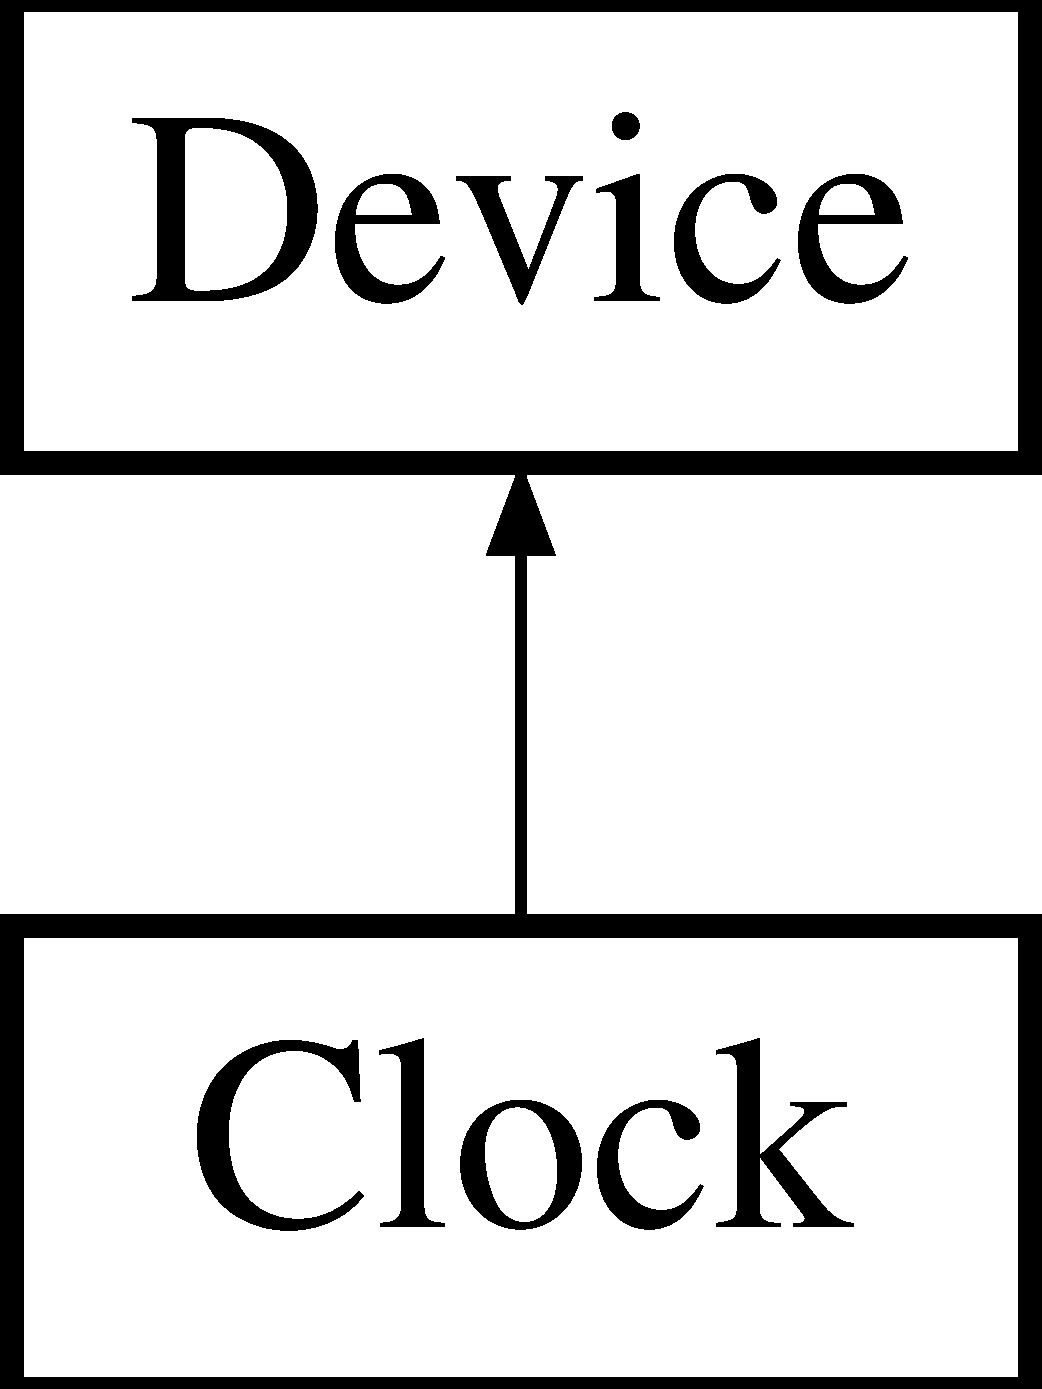
\includegraphics[height=2.000000cm]{classClock}
\end{center}
\end{figure}
\subsection*{Métodos Públicos}
\begin{DoxyCompactItemize}
\item 
\hyperlink{classClock_adbc370eb6b5f8d01645cf440188160a8}{Clock} ()
\item 
void \hyperlink{classClock_ad9e99b2538716b36b3a8fdc7d753f3a2}{begin} ()
\begin{DoxyCompactList}\small\item\em Inicializa o dispositivo. \end{DoxyCompactList}\item 
void \hyperlink{classClock_a0b77c3e7f33eb7ae0f018e469d96a250}{stop} ()
\begin{DoxyCompactList}\small\item\em Interrompe o funcionamento do dispositivo. \end{DoxyCompactList}\item 
void \hyperlink{classClock_a0ab5423b0a997aa13d7b6131c46d1358}{reset} ()
\begin{DoxyCompactList}\small\item\em Redefine o estado do dispositivo. \end{DoxyCompactList}\item 
void \hyperlink{classClock_ae7c6708cf04b233655b501a97bb1e802}{update} ()
\begin{DoxyCompactList}\small\item\em Atualiza o estado atual do dispositivo. \end{DoxyCompactList}\item 
bool \hyperlink{classClock_a16ee92e4eb0c0e3fcb7880b1256fd5ec}{is\-Ready} ()
\begin{DoxyCompactList}\small\item\em Verifica se o dispositivo está pronto para receber novos comandos ou leituras. \end{DoxyCompactList}\item 
uint8\-\_\-t \hyperlink{classClock_a3027e265e43f1d6e07d390c65aef5ecb}{get} (uint8\-\_\-t $\ast$buffer, uint8\-\_\-t size)
\item 
void \hyperlink{classClock_a296c2478ec80555af73955e09777fa5e}{set} (const uint8\-\_\-t $\ast$data, uint8\-\_\-t size)
\item 
void \hyperlink{classClock_ada8bcb5827416803dc9c7379604c18d1}{add} (\hyperlink{Clock_8h_ae646ae1606f53892b8112edd8f8ab903}{Timer} \&timer)
\begin{DoxyCompactList}\small\item\em Adiciona um novo timer. \end{DoxyCompactList}\item 
void \hyperlink{classClock_a0142f038c534c87fd38a3424c933a4c4}{remove} (\hyperlink{Clock_8h_ae646ae1606f53892b8112edd8f8ab903}{Timer} \&timer)
\begin{DoxyCompactList}\small\item\em Remove um timer. \end{DoxyCompactList}\item 
float \hyperlink{classClock_a7344905a062d17ed3d2aaa0a3a16aeb9}{get\-Accuracy} ()
\item 
uint16\-\_\-t \hyperlink{classClock_aa310ea26ad86941a3bd7ff0c2c9e4c64}{get\-Last\-Delta\-T} ()
\end{DoxyCompactItemize}


\subsection{Construtores \& Destrutores}
\hypertarget{classClock_adbc370eb6b5f8d01645cf440188160a8}{\index{Clock@{Clock}!Clock@{Clock}}
\index{Clock@{Clock}!Clock@{Clock}}
\subsubsection[{Clock}]{\setlength{\rightskip}{0pt plus 5cm}Clock\-::\-Clock (
\begin{DoxyParamCaption}
{}
\end{DoxyParamCaption}
)\hspace{0.3cm}{\ttfamily [inline]}}}\label{classClock_adbc370eb6b5f8d01645cf440188160a8}


\subsection{Métodos}
\hypertarget{classClock_ada8bcb5827416803dc9c7379604c18d1}{\index{Clock@{Clock}!add@{add}}
\index{add@{add}!Clock@{Clock}}
\subsubsection[{add}]{\setlength{\rightskip}{0pt plus 5cm}void Clock\-::add (
\begin{DoxyParamCaption}
\item[{{\bf Timer} \&}]{timer}
\end{DoxyParamCaption}
)}}\label{classClock_ada8bcb5827416803dc9c7379604c18d1}


Adiciona um novo timer. 

O relógio global decrementa o valor de \hyperlink{classClock_aa310ea26ad86941a3bd7ff0c2c9e4c64}{Clock\-::get\-Last\-Delta\-T()} para cada \hyperlink{classClock_ae7c6708cf04b233655b501a97bb1e802}{Clock\-::update()}.


\begin{DoxyParams}{Parâmetros}
{\em timer} & \\
\hline
\end{DoxyParams}
\hypertarget{classClock_ad9e99b2538716b36b3a8fdc7d753f3a2}{\index{Clock@{Clock}!begin@{begin}}
\index{begin@{begin}!Clock@{Clock}}
\subsubsection[{begin}]{\setlength{\rightskip}{0pt plus 5cm}void Clock\-::begin (
\begin{DoxyParamCaption}
{}
\end{DoxyParamCaption}
)\hspace{0.3cm}{\ttfamily [virtual]}}}\label{classClock_ad9e99b2538716b36b3a8fdc7d753f3a2}


Inicializa o dispositivo. 

Esta função é executada apenas uma vez em \hyperlink{classRobot_a6c7ee2437ae5427a19f2de4903ca0df9}{Robot\-::begin()}. 

Implementa \hyperlink{classDevice_a0dc99b16a220489d787a1cbcef4875d9}{Device}.

\hypertarget{classClock_a3027e265e43f1d6e07d390c65aef5ecb}{\index{Clock@{Clock}!get@{get}}
\index{get@{get}!Clock@{Clock}}
\subsubsection[{get}]{\setlength{\rightskip}{0pt plus 5cm}uint8\-\_\-t Clock\-::get (
\begin{DoxyParamCaption}
\item[{uint8\-\_\-t $\ast$}]{buffer, }
\item[{uint8\-\_\-t}]{size}
\end{DoxyParamCaption}
)\hspace{0.3cm}{\ttfamily [virtual]}}}\label{classClock_a3027e265e43f1d6e07d390c65aef5ecb}

\begin{DoxyParams}[1]{Parâmetros}
\mbox{\tt out}  & {\em buffer} & Array de bytes com tamanho suficiente para armazenar a resposta. \\
\hline
 & {\em size} & Tamanho do {\ttfamily buffer}.\\
\hline
\end{DoxyParams}
\begin{DoxyReturn}{Retorna}
O numero de bytes escritos em {\ttfamily buffer}. 
\end{DoxyReturn}


Implementa \hyperlink{classDevice_a0057af09515609c289d5da3be19dcc8d}{Device}.

\hypertarget{classClock_a7344905a062d17ed3d2aaa0a3a16aeb9}{\index{Clock@{Clock}!get\-Accuracy@{get\-Accuracy}}
\index{get\-Accuracy@{get\-Accuracy}!Clock@{Clock}}
\subsubsection[{get\-Accuracy}]{\setlength{\rightskip}{0pt plus 5cm}float Clock\-::get\-Accuracy (
\begin{DoxyParamCaption}
{}
\end{DoxyParamCaption}
)}}\label{classClock_a7344905a062d17ed3d2aaa0a3a16aeb9}
\hypertarget{classClock_aa310ea26ad86941a3bd7ff0c2c9e4c64}{\index{Clock@{Clock}!get\-Last\-Delta\-T@{get\-Last\-Delta\-T}}
\index{get\-Last\-Delta\-T@{get\-Last\-Delta\-T}!Clock@{Clock}}
\subsubsection[{get\-Last\-Delta\-T}]{\setlength{\rightskip}{0pt plus 5cm}uint16\-\_\-t Clock\-::get\-Last\-Delta\-T (
\begin{DoxyParamCaption}
{}
\end{DoxyParamCaption}
)}}\label{classClock_aa310ea26ad86941a3bd7ff0c2c9e4c64}
\begin{DoxyReturn}{Retorna}
O tempo gasto durante o ultimo \hyperlink{classRobot_aa50d73cd1109a70133af442674ed3a1a}{Robot\-::step()}. 
\end{DoxyReturn}
\hypertarget{classClock_a16ee92e4eb0c0e3fcb7880b1256fd5ec}{\index{Clock@{Clock}!is\-Ready@{is\-Ready}}
\index{is\-Ready@{is\-Ready}!Clock@{Clock}}
\subsubsection[{is\-Ready}]{\setlength{\rightskip}{0pt plus 5cm}bool Clock\-::is\-Ready (
\begin{DoxyParamCaption}
{}
\end{DoxyParamCaption}
)\hspace{0.3cm}{\ttfamily [virtual]}}}\label{classClock_a16ee92e4eb0c0e3fcb7880b1256fd5ec}


Verifica se o dispositivo está pronto para receber novos comandos ou leituras. 

É importante para \hyperlink{classRobot}{Robot} definir se uma ação de maior grau de abstração foi concluída ou não.

\begin{DoxyReturn}{Retorna}
{\ttfamily T\-R\-U\-E} se o dispositivo está ocioso. 
\end{DoxyReturn}


Implementa \hyperlink{classDevice_a30065df084d450dbaae9d68215e01e6f}{Device}.

\hypertarget{classClock_a0142f038c534c87fd38a3424c933a4c4}{\index{Clock@{Clock}!remove@{remove}}
\index{remove@{remove}!Clock@{Clock}}
\subsubsection[{remove}]{\setlength{\rightskip}{0pt plus 5cm}void Clock\-::remove (
\begin{DoxyParamCaption}
\item[{{\bf Timer} \&}]{timer}
\end{DoxyParamCaption}
)}}\label{classClock_a0142f038c534c87fd38a3424c933a4c4}


Remove um timer. 


\begin{DoxyParams}{Parâmetros}
{\em timer} & \\
\hline
\end{DoxyParams}
\hypertarget{classClock_a0ab5423b0a997aa13d7b6131c46d1358}{\index{Clock@{Clock}!reset@{reset}}
\index{reset@{reset}!Clock@{Clock}}
\subsubsection[{reset}]{\setlength{\rightskip}{0pt plus 5cm}void Clock\-::reset (
\begin{DoxyParamCaption}
{}
\end{DoxyParamCaption}
)\hspace{0.3cm}{\ttfamily [virtual]}}}\label{classClock_a0ab5423b0a997aa13d7b6131c46d1358}


Redefine o estado do dispositivo. 



Implementa \hyperlink{classDevice_a6e43162e890cb40eafb923b0c94d167a}{Device}.

\hypertarget{classClock_a296c2478ec80555af73955e09777fa5e}{\index{Clock@{Clock}!set@{set}}
\index{set@{set}!Clock@{Clock}}
\subsubsection[{set}]{\setlength{\rightskip}{0pt plus 5cm}void Clock\-::set (
\begin{DoxyParamCaption}
\item[{const uint8\-\_\-t $\ast$}]{data, }
\item[{uint8\-\_\-t}]{size}
\end{DoxyParamCaption}
)\hspace{0.3cm}{\ttfamily [virtual]}}}\label{classClock_a296c2478ec80555af73955e09777fa5e}

\begin{DoxyParams}[1]{Parâmetros}
\mbox{\tt in}  & {\em data} & Mensagem a ser processada pelo dispositivo. \\
\hline
 & {\em size} & Tamanho do vetor data. \\
\hline
\end{DoxyParams}


Implementa \hyperlink{classDevice_a3b4bf3ff761f93c024675548755586d8}{Device}.

\hypertarget{classClock_a0b77c3e7f33eb7ae0f018e469d96a250}{\index{Clock@{Clock}!stop@{stop}}
\index{stop@{stop}!Clock@{Clock}}
\subsubsection[{stop}]{\setlength{\rightskip}{0pt plus 5cm}void Clock\-::stop (
\begin{DoxyParamCaption}
{}
\end{DoxyParamCaption}
)\hspace{0.3cm}{\ttfamily [virtual]}}}\label{classClock_a0b77c3e7f33eb7ae0f018e469d96a250}


Interrompe o funcionamento do dispositivo. 



Implementa \hyperlink{classDevice_a22430f274658b04c280b5cc2d53aa1e4}{Device}.

\hypertarget{classClock_ae7c6708cf04b233655b501a97bb1e802}{\index{Clock@{Clock}!update@{update}}
\index{update@{update}!Clock@{Clock}}
\subsubsection[{update}]{\setlength{\rightskip}{0pt plus 5cm}void Clock\-::update (
\begin{DoxyParamCaption}
{}
\end{DoxyParamCaption}
)\hspace{0.3cm}{\ttfamily [virtual]}}}\label{classClock_ae7c6708cf04b233655b501a97bb1e802}


Atualiza o estado atual do dispositivo. 

Esta função é executada uma vez a cada \hyperlink{classRobot_aa50d73cd1109a70133af442674ed3a1a}{Robot\-::step()}. 

Implementa \hyperlink{classDevice_a7e5226b6341b1cf2ec04a5913b97becc}{Device}.



A documentação para esta classe foi gerada a partir dos seguintes arquivos\-:\begin{DoxyCompactItemize}
\item 
\hyperlink{Clock_8h}{Clock.\-h}\item 
\hyperlink{Clock_8cpp}{Clock.\-cpp}\end{DoxyCompactItemize}

\hypertarget{classCompass}{\section{Referência da Classe Compass}
\label{classCompass}\index{Compass@{Compass}}
}


{\ttfamily \#include $<$Compass.\-h$>$}

Diagrama de Hierarquia para Compass\-:\begin{figure}[H]
\begin{center}
\leavevmode
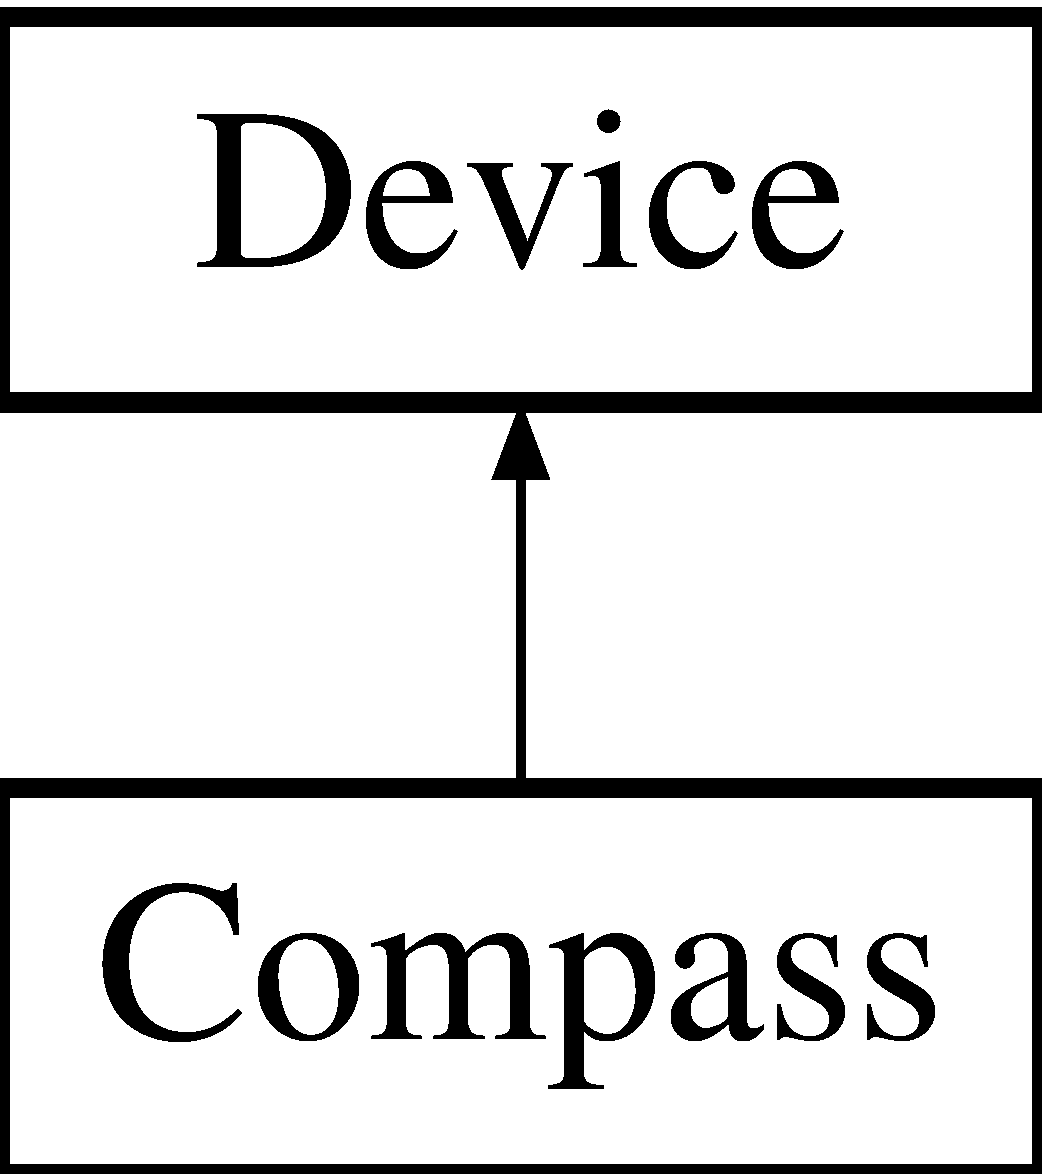
\includegraphics[height=2.000000cm]{classCompass}
\end{center}
\end{figure}
\subsection*{Métodos Públicos}
\begin{DoxyCompactItemize}
\item 
\hyperlink{classCompass_a68bd2a073cc0d461b2b46529aae04765}{Compass} ()
\item 
void \hyperlink{classCompass_a987d9ba6c1773c14a0758e46fe4dac9d}{begin} ()
\begin{DoxyCompactList}\small\item\em Inicializa o dispositivo. \end{DoxyCompactList}\item 
void \hyperlink{classCompass_a1a550ee5183625110a0444e38920723b}{stop} ()
\begin{DoxyCompactList}\small\item\em Interrompe o funcionamento do dispositivo. \end{DoxyCompactList}\item 
void \hyperlink{classCompass_aabf8451561e0748b6de05a2cbd6ab780}{reset} ()
\begin{DoxyCompactList}\small\item\em Redefine o estado do dispositivo. \end{DoxyCompactList}\item 
void \hyperlink{classCompass_a9ffa2943fec2ba6154a0f9e21cfb0b73}{update} ()
\begin{DoxyCompactList}\small\item\em Atualiza o estado atual do dispositivo. \end{DoxyCompactList}\item 
bool \hyperlink{classCompass_aec5e3e1aa8472ad7759b048d3b9522d6}{is\-Ready} ()
\begin{DoxyCompactList}\small\item\em Verifica se o dispositivo está pronto para receber novos comandos ou leituras. \end{DoxyCompactList}\item 
uint8\-\_\-t \hyperlink{classCompass_a8ed68e06b27567738cd37e4be8d0d342}{get} (uint8\-\_\-t $\ast$buffer, uint8\-\_\-t size)
\item 
void \hyperlink{classCompass_ab74dbf60e82e054f7a5d35314c89029e}{set} (const uint8\-\_\-t $\ast$data, uint8\-\_\-t size=1)
\item 
int \hyperlink{classCompass_ae431d3e75f104dab21c72968fbbd6c89}{get\-Angle} ()
\end{DoxyCompactItemize}


\subsection{Construtores \& Destrutores}
\hypertarget{classCompass_a68bd2a073cc0d461b2b46529aae04765}{\index{Compass@{Compass}!Compass@{Compass}}
\index{Compass@{Compass}!Compass@{Compass}}
\subsubsection[{Compass}]{\setlength{\rightskip}{0pt plus 5cm}Compass\-::\-Compass (
\begin{DoxyParamCaption}
{}
\end{DoxyParamCaption}
)}}\label{classCompass_a68bd2a073cc0d461b2b46529aae04765}


\subsection{Métodos}
\hypertarget{classCompass_a987d9ba6c1773c14a0758e46fe4dac9d}{\index{Compass@{Compass}!begin@{begin}}
\index{begin@{begin}!Compass@{Compass}}
\subsubsection[{begin}]{\setlength{\rightskip}{0pt plus 5cm}void Compass\-::begin (
\begin{DoxyParamCaption}
{}
\end{DoxyParamCaption}
)\hspace{0.3cm}{\ttfamily [virtual]}}}\label{classCompass_a987d9ba6c1773c14a0758e46fe4dac9d}


Inicializa o dispositivo. 

Esta função é executada apenas uma vez em \hyperlink{classRobot_a6c7ee2437ae5427a19f2de4903ca0df9}{Robot\-::begin()}. 

Implementa \hyperlink{classDevice_a0dc99b16a220489d787a1cbcef4875d9}{Device}.

\hypertarget{classCompass_a8ed68e06b27567738cd37e4be8d0d342}{\index{Compass@{Compass}!get@{get}}
\index{get@{get}!Compass@{Compass}}
\subsubsection[{get}]{\setlength{\rightskip}{0pt plus 5cm}uint8\-\_\-t Compass\-::get (
\begin{DoxyParamCaption}
\item[{uint8\-\_\-t $\ast$}]{buffer, }
\item[{uint8\-\_\-t}]{size}
\end{DoxyParamCaption}
)\hspace{0.3cm}{\ttfamily [virtual]}}}\label{classCompass_a8ed68e06b27567738cd37e4be8d0d342}

\begin{DoxyParams}[1]{Parâmetros}
\mbox{\tt out}  & {\em buffer} & Array de bytes com tamanho suficiente para armazenar a resposta. \\
\hline
 & {\em size} & Tamanho do {\ttfamily buffer}.\\
\hline
\end{DoxyParams}
\begin{DoxyReturn}{Retorna}
O numero de bytes escritos em {\ttfamily buffer}. 
\end{DoxyReturn}


Implementa \hyperlink{classDevice_a0057af09515609c289d5da3be19dcc8d}{Device}.

\hypertarget{classCompass_ae431d3e75f104dab21c72968fbbd6c89}{\index{Compass@{Compass}!get\-Angle@{get\-Angle}}
\index{get\-Angle@{get\-Angle}!Compass@{Compass}}
\subsubsection[{get\-Angle}]{\setlength{\rightskip}{0pt plus 5cm}int Compass\-::get\-Angle (
\begin{DoxyParamCaption}
{}
\end{DoxyParamCaption}
)}}\label{classCompass_ae431d3e75f104dab21c72968fbbd6c89}
\hypertarget{classCompass_aec5e3e1aa8472ad7759b048d3b9522d6}{\index{Compass@{Compass}!is\-Ready@{is\-Ready}}
\index{is\-Ready@{is\-Ready}!Compass@{Compass}}
\subsubsection[{is\-Ready}]{\setlength{\rightskip}{0pt plus 5cm}bool Compass\-::is\-Ready (
\begin{DoxyParamCaption}
{}
\end{DoxyParamCaption}
)\hspace{0.3cm}{\ttfamily [virtual]}}}\label{classCompass_aec5e3e1aa8472ad7759b048d3b9522d6}


Verifica se o dispositivo está pronto para receber novos comandos ou leituras. 

É importante para \hyperlink{classRobot}{Robot} definir se uma ação de maior grau de abstração foi concluída ou não.

\begin{DoxyReturn}{Retorna}
{\ttfamily T\-R\-U\-E} se o dispositivo está ocioso. 
\end{DoxyReturn}


Implementa \hyperlink{classDevice_a30065df084d450dbaae9d68215e01e6f}{Device}.

\hypertarget{classCompass_aabf8451561e0748b6de05a2cbd6ab780}{\index{Compass@{Compass}!reset@{reset}}
\index{reset@{reset}!Compass@{Compass}}
\subsubsection[{reset}]{\setlength{\rightskip}{0pt plus 5cm}void Compass\-::reset (
\begin{DoxyParamCaption}
{}
\end{DoxyParamCaption}
)\hspace{0.3cm}{\ttfamily [virtual]}}}\label{classCompass_aabf8451561e0748b6de05a2cbd6ab780}


Redefine o estado do dispositivo. 



Implementa \hyperlink{classDevice_a6e43162e890cb40eafb923b0c94d167a}{Device}.

\hypertarget{classCompass_ab74dbf60e82e054f7a5d35314c89029e}{\index{Compass@{Compass}!set@{set}}
\index{set@{set}!Compass@{Compass}}
\subsubsection[{set}]{\setlength{\rightskip}{0pt plus 5cm}void Compass\-::set (
\begin{DoxyParamCaption}
\item[{const uint8\-\_\-t $\ast$}]{data, }
\item[{uint8\-\_\-t}]{size = {\ttfamily 1}}
\end{DoxyParamCaption}
)\hspace{0.3cm}{\ttfamily [virtual]}}}\label{classCompass_ab74dbf60e82e054f7a5d35314c89029e}

\begin{DoxyParams}[1]{Parâmetros}
\mbox{\tt in}  & {\em data} & Mensagem a ser processada pelo dispositivo. \\
\hline
 & {\em size} & Tamanho do vetor data. \\
\hline
\end{DoxyParams}


Implementa \hyperlink{classDevice_a3b4bf3ff761f93c024675548755586d8}{Device}.

\hypertarget{classCompass_a1a550ee5183625110a0444e38920723b}{\index{Compass@{Compass}!stop@{stop}}
\index{stop@{stop}!Compass@{Compass}}
\subsubsection[{stop}]{\setlength{\rightskip}{0pt plus 5cm}void Compass\-::stop (
\begin{DoxyParamCaption}
{}
\end{DoxyParamCaption}
)\hspace{0.3cm}{\ttfamily [virtual]}}}\label{classCompass_a1a550ee5183625110a0444e38920723b}


Interrompe o funcionamento do dispositivo. 



Implementa \hyperlink{classDevice_a22430f274658b04c280b5cc2d53aa1e4}{Device}.

\hypertarget{classCompass_a9ffa2943fec2ba6154a0f9e21cfb0b73}{\index{Compass@{Compass}!update@{update}}
\index{update@{update}!Compass@{Compass}}
\subsubsection[{update}]{\setlength{\rightskip}{0pt plus 5cm}void Compass\-::update (
\begin{DoxyParamCaption}
{}
\end{DoxyParamCaption}
)\hspace{0.3cm}{\ttfamily [virtual]}}}\label{classCompass_a9ffa2943fec2ba6154a0f9e21cfb0b73}


Atualiza o estado atual do dispositivo. 

Esta função é executada uma vez a cada \hyperlink{classRobot_aa50d73cd1109a70133af442674ed3a1a}{Robot\-::step()}. 

Implementa \hyperlink{classDevice_a7e5226b6341b1cf2ec04a5913b97becc}{Device}.



A documentação para esta classe foi gerada a partir dos seguintes arquivos\-:\begin{DoxyCompactItemize}
\item 
\hyperlink{Compass_8h}{Compass.\-h}\item 
\hyperlink{Compass_8cpp}{Compass.\-cpp}\end{DoxyCompactItemize}

\hypertarget{classConnection}{\section{Referência da Classe Connection}
\label{classConnection}\index{Connection@{Connection}}
}


{\ttfamily \#include $<$Connection.\-h$>$}

Diagrama de Hierarquia para Connection\-:\begin{figure}[H]
\begin{center}
\leavevmode
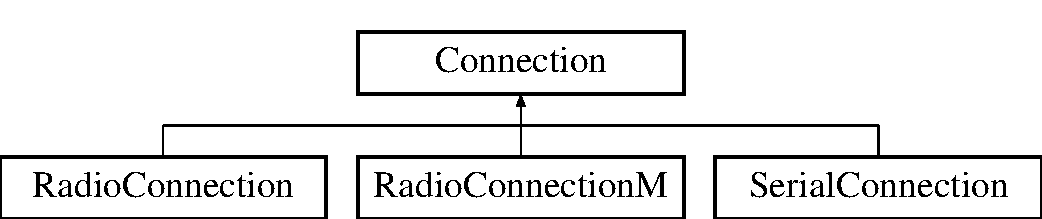
\includegraphics[height=2.000000cm]{classConnection}
\end{center}
\end{figure}
\subsection*{Métodos Públicos}
\begin{DoxyCompactItemize}
\item 
virtual void \hyperlink{classConnection_a2e5c7e67928fac5fea45e56c11d1ed31}{begin} ()=0
\begin{DoxyCompactList}\small\item\em Inicializa a conexão. \end{DoxyCompactList}\item 
virtual uint8\-\_\-t \hyperlink{classConnection_acd5ee426481b2aca2903d96f6f807341}{available} ()=0
\begin{DoxyCompactList}\small\item\em Verifica se existe alguma mensagem disponivel. \end{DoxyCompactList}\item 
virtual bool \hyperlink{classConnection_aa03e632ed6b812d915fd40dccd18a080}{send\-Message} (const uint8\-\_\-t $\ast$data, uint8\-\_\-t size)=0
\begin{DoxyCompactList}\small\item\em Envia uma mensagem. \end{DoxyCompactList}\item 
virtual uint8\-\_\-t \hyperlink{classConnection_a315961bc8327f38e4f4e09b832fc60a1}{receive\-Message} (uint8\-\_\-t $\ast$buffer, uint8\-\_\-t size)=0
\begin{DoxyCompactList}\small\item\em Recebe uma mensagem. \end{DoxyCompactList}\end{DoxyCompactItemize}


\subsection{Métodos}
\hypertarget{classConnection_acd5ee426481b2aca2903d96f6f807341}{\index{Connection@{Connection}!available@{available}}
\index{available@{available}!Connection@{Connection}}
\subsubsection[{available}]{\setlength{\rightskip}{0pt plus 5cm}virtual uint8\-\_\-t Connection\-::available (
\begin{DoxyParamCaption}
{}
\end{DoxyParamCaption}
)\hspace{0.3cm}{\ttfamily [pure virtual]}}}\label{classConnection_acd5ee426481b2aca2903d96f6f807341}


Verifica se existe alguma mensagem disponivel. 

\begin{DoxyReturn}{Retorna}
O numero de bytes disponiveis, se possivel. 
\end{DoxyReturn}


Implementado por \hyperlink{classRadioConnectionM_adfdbc2eb940e3a2a3798a76f02ea048a}{Radio\-Connection\-M}, \hyperlink{classRadioConnection_a970ffcf382ae789c22023857c5c48d83}{Radio\-Connection} e \hyperlink{classSerialConnection_a91aa59d8f0b913e91dc4ddcde8e42519}{Serial\-Connection}.

\hypertarget{classConnection_a2e5c7e67928fac5fea45e56c11d1ed31}{\index{Connection@{Connection}!begin@{begin}}
\index{begin@{begin}!Connection@{Connection}}
\subsubsection[{begin}]{\setlength{\rightskip}{0pt plus 5cm}virtual void Connection\-::begin (
\begin{DoxyParamCaption}
{}
\end{DoxyParamCaption}
)\hspace{0.3cm}{\ttfamily [pure virtual]}}}\label{classConnection_a2e5c7e67928fac5fea45e56c11d1ed31}


Inicializa a conexão. 



Implementado por \hyperlink{classSerialConnection_a6022b91cdd0bc412d8aeda364c32ce21}{Serial\-Connection}, \hyperlink{classRadioConnectionM_acbfe7d993586efe2681e8fc07dcda463}{Radio\-Connection\-M} e \hyperlink{classRadioConnection_a1deb37d098b17cfdf2c5c90e67a279aa}{Radio\-Connection}.

\hypertarget{classConnection_a315961bc8327f38e4f4e09b832fc60a1}{\index{Connection@{Connection}!receive\-Message@{receive\-Message}}
\index{receive\-Message@{receive\-Message}!Connection@{Connection}}
\subsubsection[{receive\-Message}]{\setlength{\rightskip}{0pt plus 5cm}virtual uint8\-\_\-t Connection\-::receive\-Message (
\begin{DoxyParamCaption}
\item[{uint8\-\_\-t $\ast$}]{buffer, }
\item[{uint8\-\_\-t}]{size}
\end{DoxyParamCaption}
)\hspace{0.3cm}{\ttfamily [pure virtual]}}}\label{classConnection_a315961bc8327f38e4f4e09b832fc60a1}


Recebe uma mensagem. 


\begin{DoxyParams}[1]{Parâmetros}
\mbox{\tt out}  & {\em buffer} & Um array de bytes usado para armazenar a mensagem recebida. \\
\hline
 & {\em size} & O tamanho do {\ttfamily buffer}.\\
\hline
\end{DoxyParams}
\begin{DoxyReturn}{Retorna}
O tamanho da mensagem recebida. 
\end{DoxyReturn}


Implementado por \hyperlink{classRadioConnectionM_a28ee1d2377f4d280723ce679b9f3db39}{Radio\-Connection\-M}, \hyperlink{classSerialConnection_ac72ec887122fe08fd389dc8724b31c63}{Serial\-Connection} e \hyperlink{classRadioConnection_a6dc7c7b2a7c9b5d754d73f80516a37fc}{Radio\-Connection}.

\hypertarget{classConnection_aa03e632ed6b812d915fd40dccd18a080}{\index{Connection@{Connection}!send\-Message@{send\-Message}}
\index{send\-Message@{send\-Message}!Connection@{Connection}}
\subsubsection[{send\-Message}]{\setlength{\rightskip}{0pt plus 5cm}virtual bool Connection\-::send\-Message (
\begin{DoxyParamCaption}
\item[{const uint8\-\_\-t $\ast$}]{data, }
\item[{uint8\-\_\-t}]{size}
\end{DoxyParamCaption}
)\hspace{0.3cm}{\ttfamily [pure virtual]}}}\label{classConnection_aa03e632ed6b812d915fd40dccd18a080}


Envia uma mensagem. 


\begin{DoxyParams}[1]{Parâmetros}
\mbox{\tt in}  & {\em data} & Um array de bytes contendo a mensagem. \\
\hline
 & {\em size} & O tamanho do array {\ttfamily data}.\\
\hline
\end{DoxyParams}
\begin{DoxyReturn}{Retorna}
{\ttfamily T\-R\-U\-E} se a mensagem foi entregue corretamente. 
\end{DoxyReturn}


Implementado por \hyperlink{classRadioConnection_a1bc09119403b84463264710ea40f5a4c}{Radio\-Connection}, \hyperlink{classRadioConnectionM_a8a4b19506bf383a0426023bef888e5a5}{Radio\-Connection\-M} e \hyperlink{classSerialConnection_ac98733956090bc3eaa628d156f06ef5d}{Serial\-Connection}.



A documentação para esta classe foi gerada a partir do seguinte arquivo\-:\begin{DoxyCompactItemize}
\item 
\hyperlink{Connection_8h}{Connection.\-h}\end{DoxyCompactItemize}

\hypertarget{classDevice}{\section{Referência da Classe Device}
\label{classDevice}\index{Device@{Device}}
}


{\ttfamily \#include $<$Device.\-h$>$}

Diagrama de Hierarquia para Device\-:\begin{figure}[H]
\begin{center}
\leavevmode
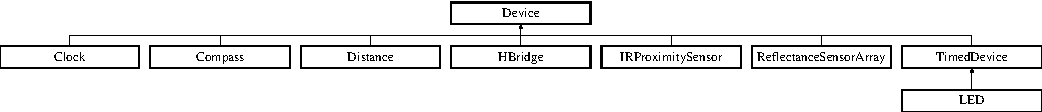
\includegraphics[height=1.500000cm]{classDevice}
\end{center}
\end{figure}
\subsection*{Métodos Públicos}
\begin{DoxyCompactItemize}
\item 
\hyperlink{classDevice_a6a343295a9f8df6dd4aa52c622a8e876}{Device} (bool \hyperlink{classDevice_a463598bce318556c79bfc0f26b38f7d3}{is\-Effector}, bool \hyperlink{classDevice_a848bce229a669a4e7531bce2b6b24154}{is\-Sensor}=false)
\begin{DoxyCompactList}\small\item\em Construtor padrão. \end{DoxyCompactList}\item 
bool \hyperlink{classDevice_a463598bce318556c79bfc0f26b38f7d3}{is\-Effector} ()
\item 
bool \hyperlink{classDevice_a848bce229a669a4e7531bce2b6b24154}{is\-Sensor} ()
\item 
uint8\-\_\-t \hyperlink{classDevice_a7b20d7fdcab77062810a0a254e978c5e}{get\-I\-D} ()
\item 
virtual void \hyperlink{classDevice_a0dc99b16a220489d787a1cbcef4875d9}{begin} ()=0
\begin{DoxyCompactList}\small\item\em Inicializa o dispositivo. \end{DoxyCompactList}\item 
virtual void \hyperlink{classDevice_a22430f274658b04c280b5cc2d53aa1e4}{stop} ()=0
\begin{DoxyCompactList}\small\item\em Interrompe o funcionamento do dispositivo. \end{DoxyCompactList}\item 
virtual void \hyperlink{classDevice_a6e43162e890cb40eafb923b0c94d167a}{reset} ()=0
\begin{DoxyCompactList}\small\item\em Redefine o estado do dispositivo. \end{DoxyCompactList}\item 
virtual void \hyperlink{classDevice_a7e5226b6341b1cf2ec04a5913b97becc}{update} ()=0
\begin{DoxyCompactList}\small\item\em Atualiza o estado atual do dispositivo. \end{DoxyCompactList}\item 
virtual bool \hyperlink{classDevice_a30065df084d450dbaae9d68215e01e6f}{is\-Ready} ()=0
\begin{DoxyCompactList}\small\item\em Verifica se o dispositivo está pronto para receber novos comandos ou leituras. \end{DoxyCompactList}\item 
virtual uint8\-\_\-t \hyperlink{classDevice_a0057af09515609c289d5da3be19dcc8d}{get} (uint8\-\_\-t $\ast$buffer, uint8\-\_\-t size)=0
\item 
virtual void \hyperlink{classDevice_a3b4bf3ff761f93c024675548755586d8}{set} (const uint8\-\_\-t $\ast$data, uint8\-\_\-t size=1)=0
\end{DoxyCompactItemize}


\subsection{Construtores \& Destrutores}
\hypertarget{classDevice_a6a343295a9f8df6dd4aa52c622a8e876}{\index{Device@{Device}!Device@{Device}}
\index{Device@{Device}!Device@{Device}}
\subsubsection[{Device}]{\setlength{\rightskip}{0pt plus 5cm}Device\-::\-Device (
\begin{DoxyParamCaption}
\item[{bool}]{is\-Effector, }
\item[{bool}]{is\-Sensor = {\ttfamily false}}
\end{DoxyParamCaption}
)}}\label{classDevice_a6a343295a9f8df6dd4aa52c622a8e876}


Construtor padrão. 


\begin{DoxyParams}{Parâmetros}
{\em is\-Effector} & Define que o dispositivo é um atuador. \\
\hline
{\em is\-Sensor} & Define que o dispositivo é um sensor. \\
\hline
\end{DoxyParams}


\subsection{Métodos}
\hypertarget{classDevice_a0dc99b16a220489d787a1cbcef4875d9}{\index{Device@{Device}!begin@{begin}}
\index{begin@{begin}!Device@{Device}}
\subsubsection[{begin}]{\setlength{\rightskip}{0pt plus 5cm}virtual void Device\-::begin (
\begin{DoxyParamCaption}
{}
\end{DoxyParamCaption}
)\hspace{0.3cm}{\ttfamily [pure virtual]}}}\label{classDevice_a0dc99b16a220489d787a1cbcef4875d9}


Inicializa o dispositivo. 

Esta função é executada apenas uma vez em \hyperlink{classRobot_a6c7ee2437ae5427a19f2de4903ca0df9}{Robot\-::begin()}. 

Implementado por \hyperlink{classClock_ad9e99b2538716b36b3a8fdc7d753f3a2}{Clock}, \hyperlink{classReflectanceSensorArray_a11602e4c9b93577608b07088f9c0fd3c}{Reflectance\-Sensor\-Array}, \hyperlink{classCompass_a987d9ba6c1773c14a0758e46fe4dac9d}{Compass}, \hyperlink{classIRProximitySensor_a84d9a5c841ffd21273762a04d791eb5a}{I\-R\-Proximity\-Sensor}, \hyperlink{classHBridge_ac0bdf510d361688b492206a64d8b2376}{H\-Bridge}, \hyperlink{classDistance_a682c993094f314fe7870813c2693c36b}{Distance} e \hyperlink{classLED_a62e402841c861af9bb4eb679f5afc7d6}{L\-E\-D}.

\hypertarget{classDevice_a0057af09515609c289d5da3be19dcc8d}{\index{Device@{Device}!get@{get}}
\index{get@{get}!Device@{Device}}
\subsubsection[{get}]{\setlength{\rightskip}{0pt plus 5cm}virtual uint8\-\_\-t Device\-::get (
\begin{DoxyParamCaption}
\item[{uint8\-\_\-t $\ast$}]{buffer, }
\item[{uint8\-\_\-t}]{size}
\end{DoxyParamCaption}
)\hspace{0.3cm}{\ttfamily [pure virtual]}}}\label{classDevice_a0057af09515609c289d5da3be19dcc8d}

\begin{DoxyParams}[1]{Parâmetros}
\mbox{\tt out}  & {\em buffer} & Array de bytes com tamanho suficiente para armazenar a resposta. \\
\hline
 & {\em size} & Tamanho do {\ttfamily buffer}.\\
\hline
\end{DoxyParams}
\begin{DoxyReturn}{Retorna}
O numero de bytes escritos em {\ttfamily buffer}. 
\end{DoxyReturn}


Implementado por \hyperlink{classClock_a3027e265e43f1d6e07d390c65aef5ecb}{Clock}, \hyperlink{classReflectanceSensorArray_ad608c5f45ea98fe65162d8c24722bc15}{Reflectance\-Sensor\-Array}, \hyperlink{classCompass_a8ed68e06b27567738cd37e4be8d0d342}{Compass}, \hyperlink{classIRProximitySensor_a7137ed31e794212c00e866af8c79b773}{I\-R\-Proximity\-Sensor}, \hyperlink{classHBridge_a87391dc065ea5b5dc6693660226cac39}{H\-Bridge}, \hyperlink{classDistance_a2735c7f7546b7fb0eba7f20940636dcc}{Distance} e \hyperlink{classLED_a70416944b6d3cae4a8dc73859a3df2aa}{L\-E\-D}.

\hypertarget{classDevice_a7b20d7fdcab77062810a0a254e978c5e}{\index{Device@{Device}!get\-I\-D@{get\-I\-D}}
\index{get\-I\-D@{get\-I\-D}!Device@{Device}}
\subsubsection[{get\-I\-D}]{\setlength{\rightskip}{0pt plus 5cm}uint8\-\_\-t Device\-::get\-I\-D (
\begin{DoxyParamCaption}
{}
\end{DoxyParamCaption}
)}}\label{classDevice_a7b20d7fdcab77062810a0a254e978c5e}
\begin{DoxyReturn}{Retorna}
O identificador exclusivo de cada dispositivo. 
\end{DoxyReturn}
\hypertarget{classDevice_a463598bce318556c79bfc0f26b38f7d3}{\index{Device@{Device}!is\-Effector@{is\-Effector}}
\index{is\-Effector@{is\-Effector}!Device@{Device}}
\subsubsection[{is\-Effector}]{\setlength{\rightskip}{0pt plus 5cm}bool Device\-::is\-Effector (
\begin{DoxyParamCaption}
{}
\end{DoxyParamCaption}
)}}\label{classDevice_a463598bce318556c79bfc0f26b38f7d3}
\begin{DoxyReturn}{Retorna}
{\ttfamily T\-R\-U\-E} se o dispositivo é um atuador. 
\end{DoxyReturn}
\hypertarget{classDevice_a30065df084d450dbaae9d68215e01e6f}{\index{Device@{Device}!is\-Ready@{is\-Ready}}
\index{is\-Ready@{is\-Ready}!Device@{Device}}
\subsubsection[{is\-Ready}]{\setlength{\rightskip}{0pt plus 5cm}virtual bool Device\-::is\-Ready (
\begin{DoxyParamCaption}
{}
\end{DoxyParamCaption}
)\hspace{0.3cm}{\ttfamily [pure virtual]}}}\label{classDevice_a30065df084d450dbaae9d68215e01e6f}


Verifica se o dispositivo está pronto para receber novos comandos ou leituras. 

É importante para \hyperlink{classRobot}{Robot} definir se uma ação de maior grau de abstração foi concluída ou não.

\begin{DoxyReturn}{Retorna}
{\ttfamily T\-R\-U\-E} se o dispositivo está ocioso. 
\end{DoxyReturn}


Implementado por \hyperlink{classClock_a16ee92e4eb0c0e3fcb7880b1256fd5ec}{Clock}, \hyperlink{classReflectanceSensorArray_a7781688e68d77cce4f7c70bbe242113b}{Reflectance\-Sensor\-Array}, \hyperlink{classCompass_aec5e3e1aa8472ad7759b048d3b9522d6}{Compass}, \hyperlink{classIRProximitySensor_a4b3faeccd653b259b513a9326c52c8dd}{I\-R\-Proximity\-Sensor}, \hyperlink{classHBridge_a3c43aac5ae38c1f04fdeb148fdfb4820}{H\-Bridge}, \hyperlink{classDistance_a16950b1595399b686fdac3c807c7ea47}{Distance} e \hyperlink{classLED_a36cc9854b853baba06ee3d1e74339c6f}{L\-E\-D}.

\hypertarget{classDevice_a848bce229a669a4e7531bce2b6b24154}{\index{Device@{Device}!is\-Sensor@{is\-Sensor}}
\index{is\-Sensor@{is\-Sensor}!Device@{Device}}
\subsubsection[{is\-Sensor}]{\setlength{\rightskip}{0pt plus 5cm}bool Device\-::is\-Sensor (
\begin{DoxyParamCaption}
{}
\end{DoxyParamCaption}
)}}\label{classDevice_a848bce229a669a4e7531bce2b6b24154}
\begin{DoxyReturn}{Retorna}
{\ttfamily T\-R\-U\-E} se o dispositivo é um sensor. 
\end{DoxyReturn}
\hypertarget{classDevice_a6e43162e890cb40eafb923b0c94d167a}{\index{Device@{Device}!reset@{reset}}
\index{reset@{reset}!Device@{Device}}
\subsubsection[{reset}]{\setlength{\rightskip}{0pt plus 5cm}virtual void Device\-::reset (
\begin{DoxyParamCaption}
{}
\end{DoxyParamCaption}
)\hspace{0.3cm}{\ttfamily [pure virtual]}}}\label{classDevice_a6e43162e890cb40eafb923b0c94d167a}


Redefine o estado do dispositivo. 



Implementado por \hyperlink{classClock_a0ab5423b0a997aa13d7b6131c46d1358}{Clock}, \hyperlink{classReflectanceSensorArray_aed9eaebad7add3ac016ea8af942261a5}{Reflectance\-Sensor\-Array}, \hyperlink{classCompass_aabf8451561e0748b6de05a2cbd6ab780}{Compass}, \hyperlink{classIRProximitySensor_aca3e197dd2cce038658bb381ad8a2d97}{I\-R\-Proximity\-Sensor}, \hyperlink{classHBridge_ad4d86b71b6ece44b30170b439b5e170f}{H\-Bridge}, \hyperlink{classDistance_a53661de88754833d8d2d26f7f0b4c158}{Distance} e \hyperlink{classLED_a8b85489d7bcfc54252f28abc0a5ba3cf}{L\-E\-D}.

\hypertarget{classDevice_a3b4bf3ff761f93c024675548755586d8}{\index{Device@{Device}!set@{set}}
\index{set@{set}!Device@{Device}}
\subsubsection[{set}]{\setlength{\rightskip}{0pt plus 5cm}virtual void Device\-::set (
\begin{DoxyParamCaption}
\item[{const uint8\-\_\-t $\ast$}]{data, }
\item[{uint8\-\_\-t}]{size = {\ttfamily 1}}
\end{DoxyParamCaption}
)\hspace{0.3cm}{\ttfamily [pure virtual]}}}\label{classDevice_a3b4bf3ff761f93c024675548755586d8}

\begin{DoxyParams}[1]{Parâmetros}
\mbox{\tt in}  & {\em data} & Mensagem a ser processada pelo dispositivo. \\
\hline
 & {\em size} & Tamanho do vetor data. \\
\hline
\end{DoxyParams}


Implementado por \hyperlink{classClock_a296c2478ec80555af73955e09777fa5e}{Clock}, \hyperlink{classReflectanceSensorArray_a023408b8b40cea4a74c5c1837a39d701}{Reflectance\-Sensor\-Array}, \hyperlink{classCompass_ab74dbf60e82e054f7a5d35314c89029e}{Compass}, \hyperlink{classIRProximitySensor_afbbfaa05fc2a2bca5b3877f99e6b0a4f}{I\-R\-Proximity\-Sensor}, \hyperlink{classHBridge_a95099e4fbaf37e9ca13de8f6af9605c9}{H\-Bridge}, \hyperlink{classDistance_abcc40ce3c92dc203c282c1d9c15ee0ee}{Distance} e \hyperlink{classLED_aae83a677cee4ee5cb952ccbb22e57781}{L\-E\-D}.

\hypertarget{classDevice_a22430f274658b04c280b5cc2d53aa1e4}{\index{Device@{Device}!stop@{stop}}
\index{stop@{stop}!Device@{Device}}
\subsubsection[{stop}]{\setlength{\rightskip}{0pt plus 5cm}virtual void Device\-::stop (
\begin{DoxyParamCaption}
{}
\end{DoxyParamCaption}
)\hspace{0.3cm}{\ttfamily [pure virtual]}}}\label{classDevice_a22430f274658b04c280b5cc2d53aa1e4}


Interrompe o funcionamento do dispositivo. 



Implementado por \hyperlink{classClock_a0b77c3e7f33eb7ae0f018e469d96a250}{Clock}, \hyperlink{classReflectanceSensorArray_ae83ddbd02df0b879bf67c99a02341f2b}{Reflectance\-Sensor\-Array}, \hyperlink{classCompass_a1a550ee5183625110a0444e38920723b}{Compass}, \hyperlink{classIRProximitySensor_a796e2f4d29f59393d25de6b3b7e0f70b}{I\-R\-Proximity\-Sensor}, \hyperlink{classHBridge_ad57868053f2f0cc144a8bf80c6090052}{H\-Bridge}, \hyperlink{classDistance_a5154b05bb07f63421d61597f9408ea6c}{Distance} e \hyperlink{classLED_a11f7b87c240eb671482a7af687b0737c}{L\-E\-D}.

\hypertarget{classDevice_a7e5226b6341b1cf2ec04a5913b97becc}{\index{Device@{Device}!update@{update}}
\index{update@{update}!Device@{Device}}
\subsubsection[{update}]{\setlength{\rightskip}{0pt plus 5cm}virtual void Device\-::update (
\begin{DoxyParamCaption}
{}
\end{DoxyParamCaption}
)\hspace{0.3cm}{\ttfamily [pure virtual]}}}\label{classDevice_a7e5226b6341b1cf2ec04a5913b97becc}


Atualiza o estado atual do dispositivo. 

Esta função é executada uma vez a cada \hyperlink{classRobot_aa50d73cd1109a70133af442674ed3a1a}{Robot\-::step()}. 

Implementado por \hyperlink{classClock_ae7c6708cf04b233655b501a97bb1e802}{Clock}, \hyperlink{classReflectanceSensorArray_a3a5f7c29c3a72026365df9cf9791e3e5}{Reflectance\-Sensor\-Array}, \hyperlink{classCompass_a9ffa2943fec2ba6154a0f9e21cfb0b73}{Compass}, \hyperlink{classIRProximitySensor_a2e18942667a104cc3aae96dc5724097e}{I\-R\-Proximity\-Sensor}, \hyperlink{classHBridge_aa6f6151443b9e6013fc5691504851e58}{H\-Bridge}, \hyperlink{classDistance_a1bc009e64442db5e875af76ae29ae57f}{Distance} e \hyperlink{classLED_ad615d612f5b0c7dac4dde5245f191382}{L\-E\-D}.



A documentação para esta classe foi gerada a partir dos seguintes arquivos\-:\begin{DoxyCompactItemize}
\item 
\hyperlink{Device_8h}{Device.\-h}\item 
\hyperlink{Device_8cpp}{Device.\-cpp}\end{DoxyCompactItemize}

\hypertarget{classDistance}{\section{Referência da Classe Distance}
\label{classDistance}\index{Distance@{Distance}}
}


{\ttfamily \#include $<$Distance.\-h$>$}

Diagrama de Hierarquia para Distance\-:\begin{figure}[H]
\begin{center}
\leavevmode
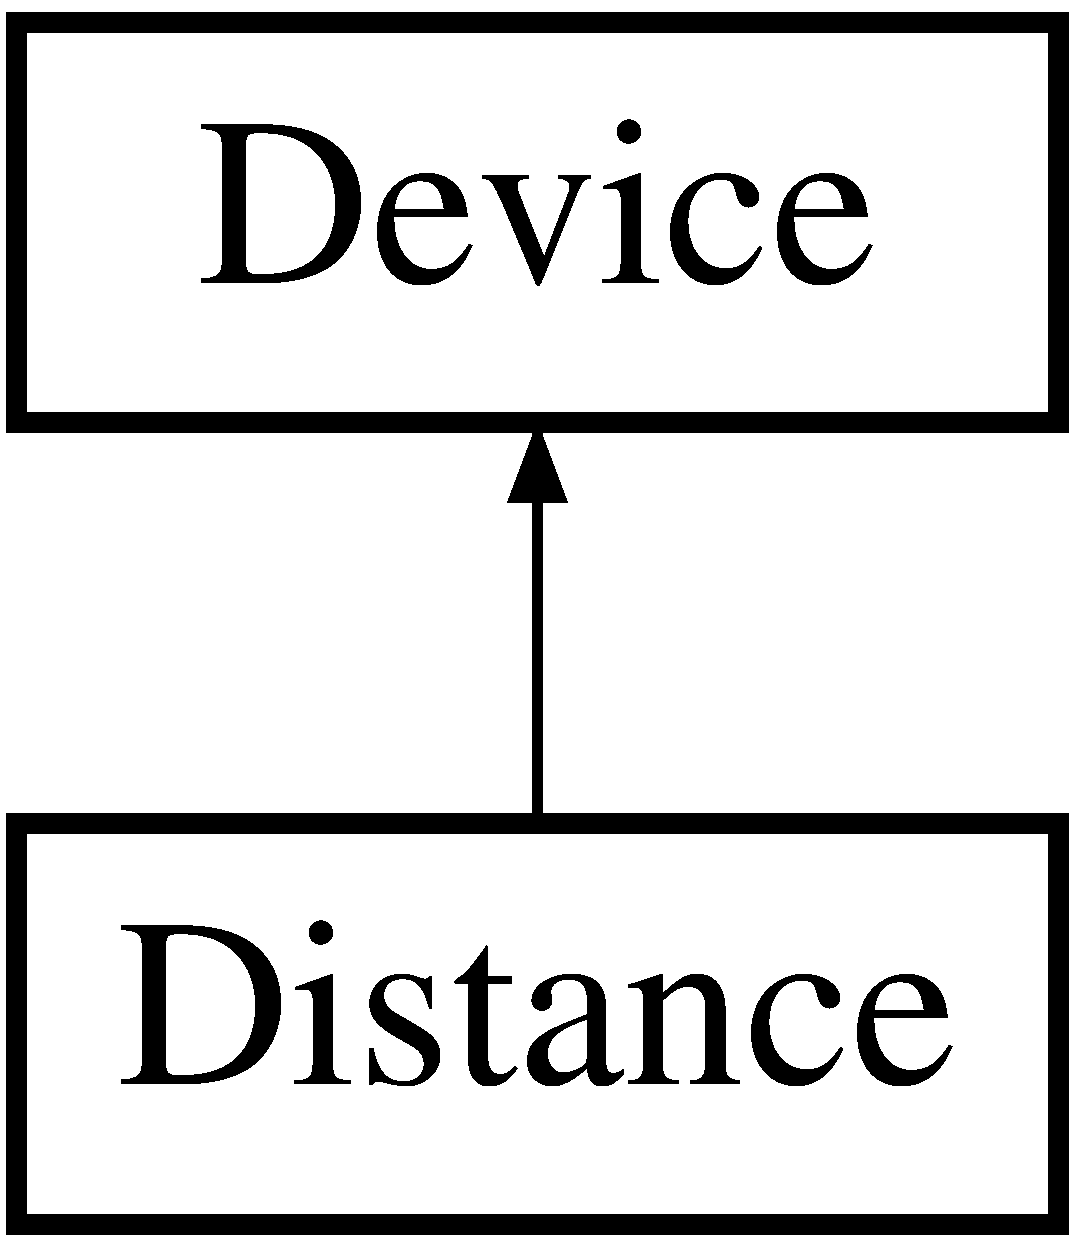
\includegraphics[height=2.000000cm]{classDistance}
\end{center}
\end{figure}
\subsection*{Métodos Públicos}
\begin{DoxyCompactItemize}
\item 
\hyperlink{classDistance_a2c4329362399da0e97f431f97757cf1d}{Distance} (uint8\-\_\-t pin)
\item 
void \hyperlink{classDistance_a682c993094f314fe7870813c2693c36b}{begin} ()
\begin{DoxyCompactList}\small\item\em Inicializa o dispositivo. \end{DoxyCompactList}\item 
void \hyperlink{classDistance_a5154b05bb07f63421d61597f9408ea6c}{stop} ()
\begin{DoxyCompactList}\small\item\em Interrompe o funcionamento do dispositivo. \end{DoxyCompactList}\item 
void \hyperlink{classDistance_a53661de88754833d8d2d26f7f0b4c158}{reset} ()
\begin{DoxyCompactList}\small\item\em Redefine o estado do dispositivo. \end{DoxyCompactList}\item 
void \hyperlink{classDistance_a1bc009e64442db5e875af76ae29ae57f}{update} ()
\begin{DoxyCompactList}\small\item\em Atualiza o estado atual do dispositivo. \end{DoxyCompactList}\item 
bool \hyperlink{classDistance_a16950b1595399b686fdac3c807c7ea47}{is\-Ready} ()
\begin{DoxyCompactList}\small\item\em Verifica se o dispositivo está pronto para receber novos comandos ou leituras. \end{DoxyCompactList}\item 
uint8\-\_\-t \hyperlink{classDistance_a2735c7f7546b7fb0eba7f20940636dcc}{get} (uint8\-\_\-t $\ast$buffer, uint8\-\_\-t size)
\item 
void \hyperlink{classDistance_abcc40ce3c92dc203c282c1d9c15ee0ee}{set} (const uint8\-\_\-t $\ast$data, uint8\-\_\-t size=1)
\end{DoxyCompactItemize}


\subsection{Construtores \& Destrutores}
\hypertarget{classDistance_a2c4329362399da0e97f431f97757cf1d}{\index{Distance@{Distance}!Distance@{Distance}}
\index{Distance@{Distance}!Distance@{Distance}}
\subsubsection[{Distance}]{\setlength{\rightskip}{0pt plus 5cm}Distance\-::\-Distance (
\begin{DoxyParamCaption}
\item[{uint8\-\_\-t}]{pin}
\end{DoxyParamCaption}
)}}\label{classDistance_a2c4329362399da0e97f431f97757cf1d}


\subsection{Métodos}
\hypertarget{classDistance_a682c993094f314fe7870813c2693c36b}{\index{Distance@{Distance}!begin@{begin}}
\index{begin@{begin}!Distance@{Distance}}
\subsubsection[{begin}]{\setlength{\rightskip}{0pt plus 5cm}void Distance\-::begin (
\begin{DoxyParamCaption}
{}
\end{DoxyParamCaption}
)\hspace{0.3cm}{\ttfamily [virtual]}}}\label{classDistance_a682c993094f314fe7870813c2693c36b}


Inicializa o dispositivo. 

Esta função é executada apenas uma vez em \hyperlink{classRobot_a6c7ee2437ae5427a19f2de4903ca0df9}{Robot\-::begin()}. 

Implementa \hyperlink{classDevice_a0dc99b16a220489d787a1cbcef4875d9}{Device}.

\hypertarget{classDistance_a2735c7f7546b7fb0eba7f20940636dcc}{\index{Distance@{Distance}!get@{get}}
\index{get@{get}!Distance@{Distance}}
\subsubsection[{get}]{\setlength{\rightskip}{0pt plus 5cm}uint8\-\_\-t Distance\-::get (
\begin{DoxyParamCaption}
\item[{uint8\-\_\-t $\ast$}]{buffer, }
\item[{uint8\-\_\-t}]{size}
\end{DoxyParamCaption}
)\hspace{0.3cm}{\ttfamily [virtual]}}}\label{classDistance_a2735c7f7546b7fb0eba7f20940636dcc}

\begin{DoxyParams}[1]{Parâmetros}
\mbox{\tt out}  & {\em buffer} & Array de bytes com tamanho suficiente para armazenar a resposta. \\
\hline
 & {\em size} & Tamanho do {\ttfamily buffer}.\\
\hline
\end{DoxyParams}
\begin{DoxyReturn}{Retorna}
O numero de bytes escritos em {\ttfamily buffer}. 
\end{DoxyReturn}


Implementa \hyperlink{classDevice_a0057af09515609c289d5da3be19dcc8d}{Device}.

\hypertarget{classDistance_a16950b1595399b686fdac3c807c7ea47}{\index{Distance@{Distance}!is\-Ready@{is\-Ready}}
\index{is\-Ready@{is\-Ready}!Distance@{Distance}}
\subsubsection[{is\-Ready}]{\setlength{\rightskip}{0pt plus 5cm}bool Distance\-::is\-Ready (
\begin{DoxyParamCaption}
{}
\end{DoxyParamCaption}
)\hspace{0.3cm}{\ttfamily [virtual]}}}\label{classDistance_a16950b1595399b686fdac3c807c7ea47}


Verifica se o dispositivo está pronto para receber novos comandos ou leituras. 

É importante para \hyperlink{classRobot}{Robot} definir se uma ação de maior grau de abstração foi concluída ou não.

\begin{DoxyReturn}{Retorna}
{\ttfamily T\-R\-U\-E} se o dispositivo está ocioso. 
\end{DoxyReturn}


Implementa \hyperlink{classDevice_a30065df084d450dbaae9d68215e01e6f}{Device}.

\hypertarget{classDistance_a53661de88754833d8d2d26f7f0b4c158}{\index{Distance@{Distance}!reset@{reset}}
\index{reset@{reset}!Distance@{Distance}}
\subsubsection[{reset}]{\setlength{\rightskip}{0pt plus 5cm}void Distance\-::reset (
\begin{DoxyParamCaption}
{}
\end{DoxyParamCaption}
)\hspace{0.3cm}{\ttfamily [virtual]}}}\label{classDistance_a53661de88754833d8d2d26f7f0b4c158}


Redefine o estado do dispositivo. 



Implementa \hyperlink{classDevice_a6e43162e890cb40eafb923b0c94d167a}{Device}.

\hypertarget{classDistance_abcc40ce3c92dc203c282c1d9c15ee0ee}{\index{Distance@{Distance}!set@{set}}
\index{set@{set}!Distance@{Distance}}
\subsubsection[{set}]{\setlength{\rightskip}{0pt plus 5cm}void Distance\-::set (
\begin{DoxyParamCaption}
\item[{const uint8\-\_\-t $\ast$}]{data, }
\item[{uint8\-\_\-t}]{size = {\ttfamily 1}}
\end{DoxyParamCaption}
)\hspace{0.3cm}{\ttfamily [virtual]}}}\label{classDistance_abcc40ce3c92dc203c282c1d9c15ee0ee}

\begin{DoxyParams}[1]{Parâmetros}
\mbox{\tt in}  & {\em data} & Mensagem a ser processada pelo dispositivo. \\
\hline
 & {\em size} & Tamanho do vetor data. \\
\hline
\end{DoxyParams}


Implementa \hyperlink{classDevice_a3b4bf3ff761f93c024675548755586d8}{Device}.

\hypertarget{classDistance_a5154b05bb07f63421d61597f9408ea6c}{\index{Distance@{Distance}!stop@{stop}}
\index{stop@{stop}!Distance@{Distance}}
\subsubsection[{stop}]{\setlength{\rightskip}{0pt plus 5cm}void Distance\-::stop (
\begin{DoxyParamCaption}
{}
\end{DoxyParamCaption}
)\hspace{0.3cm}{\ttfamily [virtual]}}}\label{classDistance_a5154b05bb07f63421d61597f9408ea6c}


Interrompe o funcionamento do dispositivo. 



Implementa \hyperlink{classDevice_a22430f274658b04c280b5cc2d53aa1e4}{Device}.

\hypertarget{classDistance_a1bc009e64442db5e875af76ae29ae57f}{\index{Distance@{Distance}!update@{update}}
\index{update@{update}!Distance@{Distance}}
\subsubsection[{update}]{\setlength{\rightskip}{0pt plus 5cm}void Distance\-::update (
\begin{DoxyParamCaption}
{}
\end{DoxyParamCaption}
)\hspace{0.3cm}{\ttfamily [virtual]}}}\label{classDistance_a1bc009e64442db5e875af76ae29ae57f}


Atualiza o estado atual do dispositivo. 

Esta função é executada uma vez a cada \hyperlink{classRobot_aa50d73cd1109a70133af442674ed3a1a}{Robot\-::step()}. 

Implementa \hyperlink{classDevice_a7e5226b6341b1cf2ec04a5913b97becc}{Device}.



A documentação para esta classe foi gerada a partir dos seguintes arquivos\-:\begin{DoxyCompactItemize}
\item 
\hyperlink{Distance_8h}{Distance.\-h}\item 
\hyperlink{Distance_8cpp}{Distance.\-cpp}\end{DoxyCompactItemize}

\hypertarget{classGenericRobot}{\section{Referência da Classe Generic\-Robot}
\label{classGenericRobot}\index{Generic\-Robot@{Generic\-Robot}}
}


{\ttfamily \#include $<$Generic\-Robot.\-h$>$}

Diagrama de Hierarquia para Generic\-Robot\-:\begin{figure}[H]
\begin{center}
\leavevmode
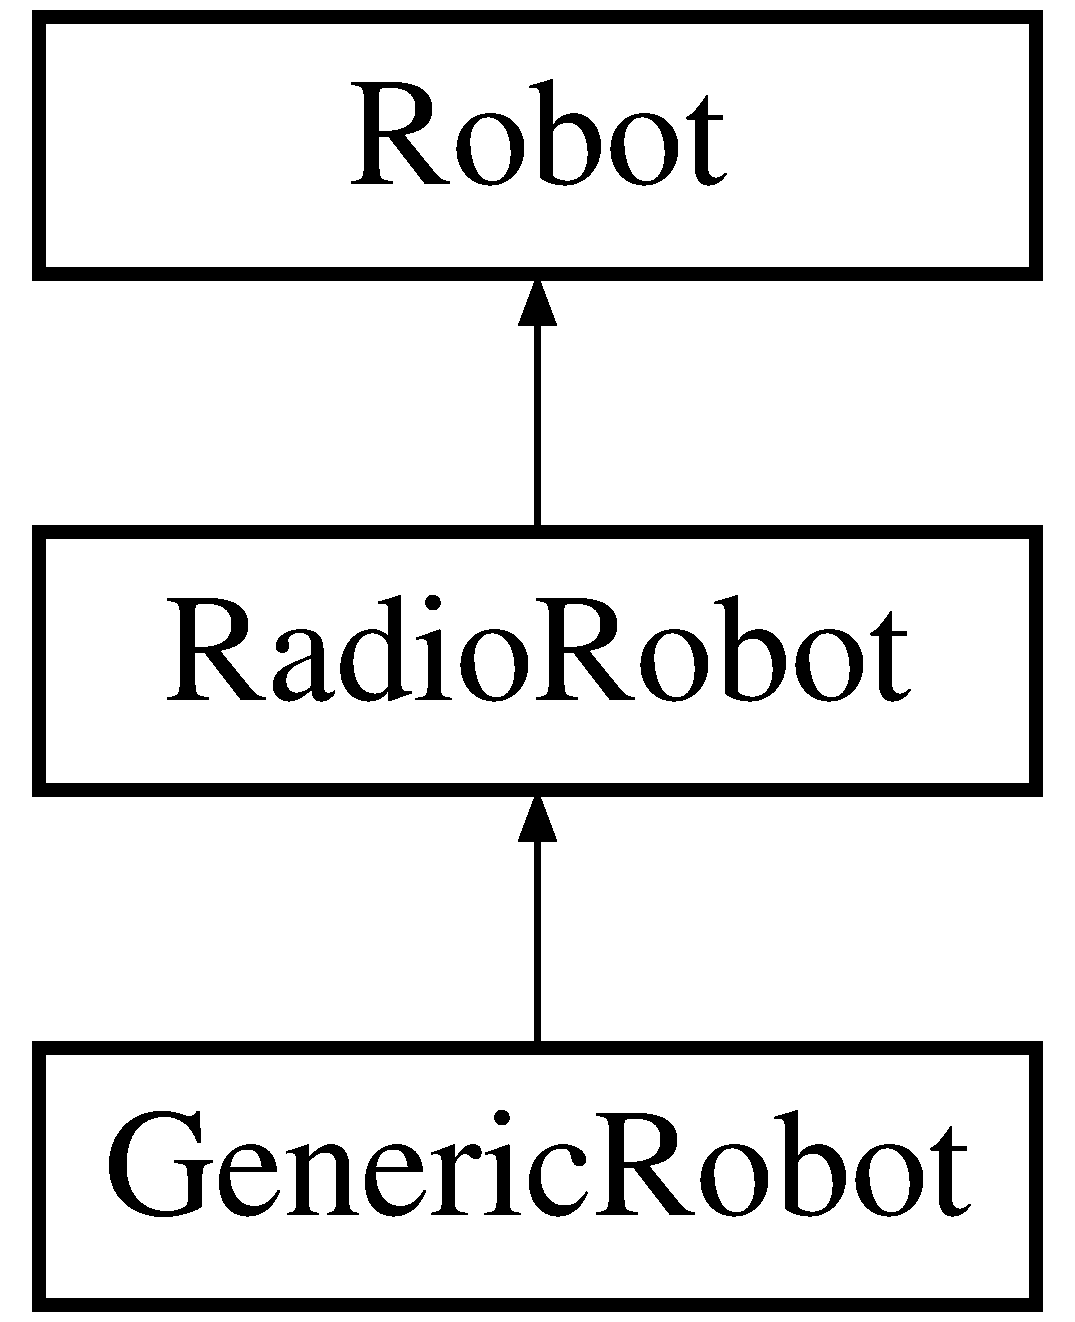
\includegraphics[height=3.000000cm]{classGenericRobot}
\end{center}
\end{figure}
\subsection*{Métodos Públicos}
\begin{DoxyCompactItemize}
\item 
\hyperlink{classGenericRobot_a99cc522b01d27497565760c5d11b0871}{Generic\-Robot} ()
\item 
\hyperlink{classDevice}{Device} $\ast$ \hyperlink{classGenericRobot_a4eac111dafabbfb130ca988e06a18808}{create\-New} (uint8\-\_\-t id, const uint8\-\_\-t $\ast$data, uint8\-\_\-t size)
\end{DoxyCompactItemize}
\subsection*{Additional Inherited Members}


\subsection{Construtores \& Destrutores}
\hypertarget{classGenericRobot_a99cc522b01d27497565760c5d11b0871}{\index{Generic\-Robot@{Generic\-Robot}!Generic\-Robot@{Generic\-Robot}}
\index{Generic\-Robot@{Generic\-Robot}!GenericRobot@{Generic\-Robot}}
\subsubsection[{Generic\-Robot}]{\setlength{\rightskip}{0pt plus 5cm}Generic\-Robot\-::\-Generic\-Robot (
\begin{DoxyParamCaption}
{}
\end{DoxyParamCaption}
)\hspace{0.3cm}{\ttfamily [inline]}}}\label{classGenericRobot_a99cc522b01d27497565760c5d11b0871}


\subsection{Métodos}
\hypertarget{classGenericRobot_a4eac111dafabbfb130ca988e06a18808}{\index{Generic\-Robot@{Generic\-Robot}!create\-New@{create\-New}}
\index{create\-New@{create\-New}!GenericRobot@{Generic\-Robot}}
\subsubsection[{create\-New}]{\setlength{\rightskip}{0pt plus 5cm}{\bf Device} $\ast$ Generic\-Robot\-::create\-New (
\begin{DoxyParamCaption}
\item[{uint8\-\_\-t}]{id, }
\item[{const uint8\-\_\-t $\ast$}]{data, }
\item[{uint8\-\_\-t}]{size}
\end{DoxyParamCaption}
)\hspace{0.3cm}{\ttfamily [virtual]}}}\label{classGenericRobot_a4eac111dafabbfb130ca988e06a18808}


Reimplementação de \hyperlink{classRadioRobot_ae52a4b2243df9d55238cfaa7be2e302d}{Radio\-Robot}.



A documentação para esta classe foi gerada a partir dos seguintes arquivos\-:\begin{DoxyCompactItemize}
\item 
\hyperlink{GenericRobot_8h}{Generic\-Robot.\-h}\item 
\hyperlink{GenericRobot_8cpp}{Generic\-Robot.\-cpp}\end{DoxyCompactItemize}

\hypertarget{classHBridge}{\section{Referência da Classe H\-Bridge}
\label{classHBridge}\index{H\-Bridge@{H\-Bridge}}
}


{\ttfamily \#include $<$H\-Bridge.\-h$>$}

Diagrama de Hierarquia para H\-Bridge\-:\begin{figure}[H]
\begin{center}
\leavevmode
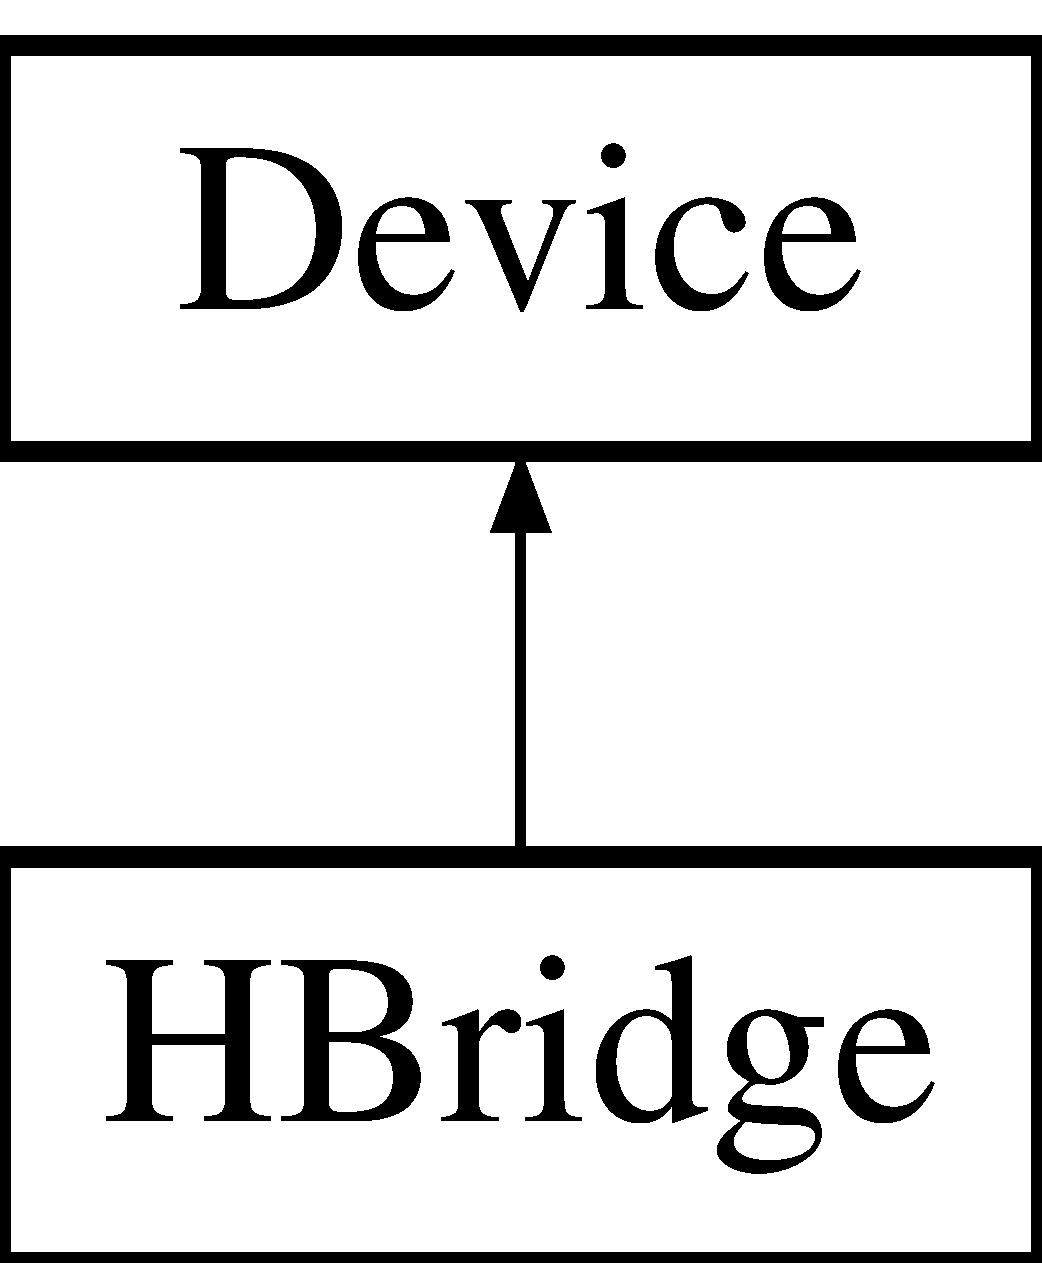
\includegraphics[height=2.000000cm]{classHBridge}
\end{center}
\end{figure}
\subsection*{Métodos Públicos}
\begin{DoxyCompactItemize}
\item 
\hyperlink{classHBridge_a7030e8d12de11cc71ab9945191fafa1c}{H\-Bridge} (uint8\-\_\-t pin1, uint8\-\_\-t pin2, uint8\-\_\-t pin3, uint8\-\_\-t pin4)
\item 
void \hyperlink{classHBridge_ac0bdf510d361688b492206a64d8b2376}{begin} ()
\begin{DoxyCompactList}\small\item\em Inicializa o dispositivo. \end{DoxyCompactList}\item 
void \hyperlink{classHBridge_ad57868053f2f0cc144a8bf80c6090052}{stop} ()
\begin{DoxyCompactList}\small\item\em Interrompe o funcionamento do dispositivo. \end{DoxyCompactList}\item 
void \hyperlink{classHBridge_ad4d86b71b6ece44b30170b439b5e170f}{reset} ()
\begin{DoxyCompactList}\small\item\em Redefine o estado do dispositivo. \end{DoxyCompactList}\item 
void \hyperlink{classHBridge_aa6f6151443b9e6013fc5691504851e58}{update} ()
\begin{DoxyCompactList}\small\item\em Atualiza o estado atual do dispositivo. \end{DoxyCompactList}\item 
bool \hyperlink{classHBridge_a3c43aac5ae38c1f04fdeb148fdfb4820}{is\-Ready} ()
\begin{DoxyCompactList}\small\item\em Verifica se o dispositivo está pronto para receber novos comandos ou leituras. \end{DoxyCompactList}\item 
uint8\-\_\-t \hyperlink{classHBridge_a87391dc065ea5b5dc6693660226cac39}{get} (uint8\-\_\-t $\ast$buffer, uint8\-\_\-t size)
\item 
void \hyperlink{classHBridge_a95099e4fbaf37e9ca13de8f6af9605c9}{set} (const uint8\-\_\-t $\ast$data, uint8\-\_\-t size=1)
\item 
void \hyperlink{classHBridge_a9d7b4166a7455698137031928926aed7}{set\-Motor\-State} (uint8\-\_\-t motor, int8\-\_\-t speed)
\end{DoxyCompactItemize}


\subsection{Construtores \& Destrutores}
\hypertarget{classHBridge_a7030e8d12de11cc71ab9945191fafa1c}{\index{H\-Bridge@{H\-Bridge}!H\-Bridge@{H\-Bridge}}
\index{H\-Bridge@{H\-Bridge}!HBridge@{H\-Bridge}}
\subsubsection[{H\-Bridge}]{\setlength{\rightskip}{0pt plus 5cm}H\-Bridge\-::\-H\-Bridge (
\begin{DoxyParamCaption}
\item[{uint8\-\_\-t}]{pin1, }
\item[{uint8\-\_\-t}]{pin2, }
\item[{uint8\-\_\-t}]{pin3, }
\item[{uint8\-\_\-t}]{pin4}
\end{DoxyParamCaption}
)}}\label{classHBridge_a7030e8d12de11cc71ab9945191fafa1c}


\subsection{Métodos}
\hypertarget{classHBridge_ac0bdf510d361688b492206a64d8b2376}{\index{H\-Bridge@{H\-Bridge}!begin@{begin}}
\index{begin@{begin}!HBridge@{H\-Bridge}}
\subsubsection[{begin}]{\setlength{\rightskip}{0pt plus 5cm}void H\-Bridge\-::begin (
\begin{DoxyParamCaption}
{}
\end{DoxyParamCaption}
)\hspace{0.3cm}{\ttfamily [virtual]}}}\label{classHBridge_ac0bdf510d361688b492206a64d8b2376}


Inicializa o dispositivo. 

Esta função é executada apenas uma vez em \hyperlink{classRobot_a6c7ee2437ae5427a19f2de4903ca0df9}{Robot\-::begin()}. 

Implementa \hyperlink{classDevice_a0dc99b16a220489d787a1cbcef4875d9}{Device}.

\hypertarget{classHBridge_a87391dc065ea5b5dc6693660226cac39}{\index{H\-Bridge@{H\-Bridge}!get@{get}}
\index{get@{get}!HBridge@{H\-Bridge}}
\subsubsection[{get}]{\setlength{\rightskip}{0pt plus 5cm}uint8\-\_\-t H\-Bridge\-::get (
\begin{DoxyParamCaption}
\item[{uint8\-\_\-t $\ast$}]{buffer, }
\item[{uint8\-\_\-t}]{size}
\end{DoxyParamCaption}
)\hspace{0.3cm}{\ttfamily [virtual]}}}\label{classHBridge_a87391dc065ea5b5dc6693660226cac39}

\begin{DoxyParams}[1]{Parâmetros}
\mbox{\tt out}  & {\em buffer} & Array de bytes com tamanho suficiente para armazenar a resposta. \\
\hline
 & {\em size} & Tamanho do {\ttfamily buffer}.\\
\hline
\end{DoxyParams}
\begin{DoxyReturn}{Retorna}
O numero de bytes escritos em {\ttfamily buffer}. 
\end{DoxyReturn}


Implementa \hyperlink{classDevice_a0057af09515609c289d5da3be19dcc8d}{Device}.

\hypertarget{classHBridge_a3c43aac5ae38c1f04fdeb148fdfb4820}{\index{H\-Bridge@{H\-Bridge}!is\-Ready@{is\-Ready}}
\index{is\-Ready@{is\-Ready}!HBridge@{H\-Bridge}}
\subsubsection[{is\-Ready}]{\setlength{\rightskip}{0pt plus 5cm}bool H\-Bridge\-::is\-Ready (
\begin{DoxyParamCaption}
{}
\end{DoxyParamCaption}
)\hspace{0.3cm}{\ttfamily [virtual]}}}\label{classHBridge_a3c43aac5ae38c1f04fdeb148fdfb4820}


Verifica se o dispositivo está pronto para receber novos comandos ou leituras. 

É importante para \hyperlink{classRobot}{Robot} definir se uma ação de maior grau de abstração foi concluída ou não.

\begin{DoxyReturn}{Retorna}
{\ttfamily T\-R\-U\-E} se o dispositivo está ocioso. 
\end{DoxyReturn}


Implementa \hyperlink{classDevice_a30065df084d450dbaae9d68215e01e6f}{Device}.

\hypertarget{classHBridge_ad4d86b71b6ece44b30170b439b5e170f}{\index{H\-Bridge@{H\-Bridge}!reset@{reset}}
\index{reset@{reset}!HBridge@{H\-Bridge}}
\subsubsection[{reset}]{\setlength{\rightskip}{0pt plus 5cm}void H\-Bridge\-::reset (
\begin{DoxyParamCaption}
{}
\end{DoxyParamCaption}
)\hspace{0.3cm}{\ttfamily [virtual]}}}\label{classHBridge_ad4d86b71b6ece44b30170b439b5e170f}


Redefine o estado do dispositivo. 



Implementa \hyperlink{classDevice_a6e43162e890cb40eafb923b0c94d167a}{Device}.

\hypertarget{classHBridge_a95099e4fbaf37e9ca13de8f6af9605c9}{\index{H\-Bridge@{H\-Bridge}!set@{set}}
\index{set@{set}!HBridge@{H\-Bridge}}
\subsubsection[{set}]{\setlength{\rightskip}{0pt plus 5cm}void H\-Bridge\-::set (
\begin{DoxyParamCaption}
\item[{const uint8\-\_\-t $\ast$}]{data, }
\item[{uint8\-\_\-t}]{size = {\ttfamily 1}}
\end{DoxyParamCaption}
)\hspace{0.3cm}{\ttfamily [virtual]}}}\label{classHBridge_a95099e4fbaf37e9ca13de8f6af9605c9}

\begin{DoxyParams}[1]{Parâmetros}
\mbox{\tt in}  & {\em data} & Mensagem a ser processada pelo dispositivo. \\
\hline
 & {\em size} & Tamanho do vetor data. \\
\hline
\end{DoxyParams}


Implementa \hyperlink{classDevice_a3b4bf3ff761f93c024675548755586d8}{Device}.

\hypertarget{classHBridge_a9d7b4166a7455698137031928926aed7}{\index{H\-Bridge@{H\-Bridge}!set\-Motor\-State@{set\-Motor\-State}}
\index{set\-Motor\-State@{set\-Motor\-State}!HBridge@{H\-Bridge}}
\subsubsection[{set\-Motor\-State}]{\setlength{\rightskip}{0pt plus 5cm}void H\-Bridge\-::set\-Motor\-State (
\begin{DoxyParamCaption}
\item[{uint8\-\_\-t}]{motor, }
\item[{int8\-\_\-t}]{speed}
\end{DoxyParamCaption}
)}}\label{classHBridge_a9d7b4166a7455698137031928926aed7}
\hypertarget{classHBridge_ad57868053f2f0cc144a8bf80c6090052}{\index{H\-Bridge@{H\-Bridge}!stop@{stop}}
\index{stop@{stop}!HBridge@{H\-Bridge}}
\subsubsection[{stop}]{\setlength{\rightskip}{0pt plus 5cm}void H\-Bridge\-::stop (
\begin{DoxyParamCaption}
{}
\end{DoxyParamCaption}
)\hspace{0.3cm}{\ttfamily [virtual]}}}\label{classHBridge_ad57868053f2f0cc144a8bf80c6090052}


Interrompe o funcionamento do dispositivo. 



Implementa \hyperlink{classDevice_a22430f274658b04c280b5cc2d53aa1e4}{Device}.

\hypertarget{classHBridge_aa6f6151443b9e6013fc5691504851e58}{\index{H\-Bridge@{H\-Bridge}!update@{update}}
\index{update@{update}!HBridge@{H\-Bridge}}
\subsubsection[{update}]{\setlength{\rightskip}{0pt plus 5cm}void H\-Bridge\-::update (
\begin{DoxyParamCaption}
{}
\end{DoxyParamCaption}
)\hspace{0.3cm}{\ttfamily [virtual]}}}\label{classHBridge_aa6f6151443b9e6013fc5691504851e58}


Atualiza o estado atual do dispositivo. 

Esta função é executada uma vez a cada \hyperlink{classRobot_aa50d73cd1109a70133af442674ed3a1a}{Robot\-::step()}. 

Implementa \hyperlink{classDevice_a7e5226b6341b1cf2ec04a5913b97becc}{Device}.



A documentação para esta classe foi gerada a partir dos seguintes arquivos\-:\begin{DoxyCompactItemize}
\item 
\hyperlink{HBridge_8h}{H\-Bridge.\-h}\item 
\hyperlink{HBridge_8cpp}{H\-Bridge.\-cpp}\end{DoxyCompactItemize}

\hypertarget{classIRProximitySensor}{\section{Referência da Classe I\-R\-Proximity\-Sensor}
\label{classIRProximitySensor}\index{I\-R\-Proximity\-Sensor@{I\-R\-Proximity\-Sensor}}
}


{\ttfamily \#include $<$I\-R\-Proximity\-Sensor.\-h$>$}

Diagrama de Hierarquia para I\-R\-Proximity\-Sensor\-:\begin{figure}[H]
\begin{center}
\leavevmode
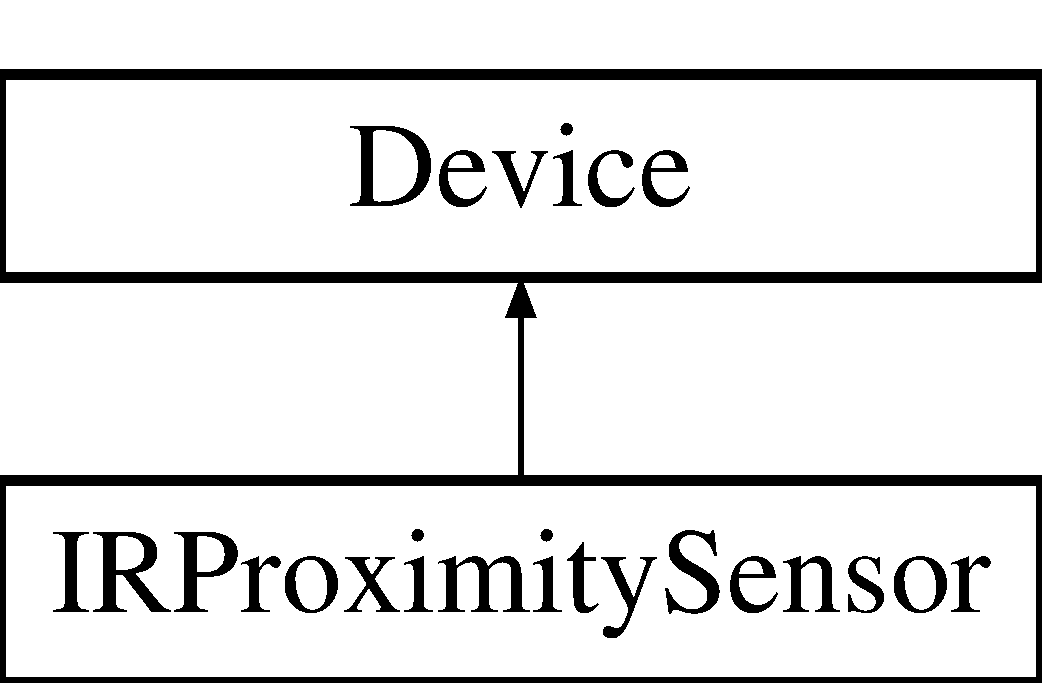
\includegraphics[height=2.000000cm]{classIRProximitySensor}
\end{center}
\end{figure}
\subsection*{Métodos Públicos}
\begin{DoxyCompactItemize}
\item 
\hyperlink{classIRProximitySensor_a8a69e6f2fd9489e3d06be8421dd2d541}{I\-R\-Proximity\-Sensor} (uint8\-\_\-t pin)
\item 
void \hyperlink{classIRProximitySensor_a84d9a5c841ffd21273762a04d791eb5a}{begin} ()
\begin{DoxyCompactList}\small\item\em Inicializa o dispositivo. \end{DoxyCompactList}\item 
void \hyperlink{classIRProximitySensor_a796e2f4d29f59393d25de6b3b7e0f70b}{stop} ()
\begin{DoxyCompactList}\small\item\em Interrompe o funcionamento do dispositivo. \end{DoxyCompactList}\item 
void \hyperlink{classIRProximitySensor_aca3e197dd2cce038658bb381ad8a2d97}{reset} ()
\begin{DoxyCompactList}\small\item\em Redefine o estado do dispositivo. \end{DoxyCompactList}\item 
void \hyperlink{classIRProximitySensor_a2e18942667a104cc3aae96dc5724097e}{update} ()
\begin{DoxyCompactList}\small\item\em Atualiza o estado atual do dispositivo. \end{DoxyCompactList}\item 
bool \hyperlink{classIRProximitySensor_a4b3faeccd653b259b513a9326c52c8dd}{is\-Ready} ()
\begin{DoxyCompactList}\small\item\em Verifica se o dispositivo está pronto para receber novos comandos ou leituras. \end{DoxyCompactList}\item 
uint8\-\_\-t \hyperlink{classIRProximitySensor_a7137ed31e794212c00e866af8c79b773}{get} (uint8\-\_\-t $\ast$buffer, uint8\-\_\-t size)
\item 
void \hyperlink{classIRProximitySensor_afbbfaa05fc2a2bca5b3877f99e6b0a4f}{set} (const uint8\-\_\-t $\ast$data, uint8\-\_\-t size=1)
\item 
int \hyperlink{classIRProximitySensor_ab9bdeff4396b6a28bb2e1717e4f3f96e}{get\-Distance} ()
\end{DoxyCompactItemize}


\subsection{Construtores \& Destrutores}
\hypertarget{classIRProximitySensor_a8a69e6f2fd9489e3d06be8421dd2d541}{\index{I\-R\-Proximity\-Sensor@{I\-R\-Proximity\-Sensor}!I\-R\-Proximity\-Sensor@{I\-R\-Proximity\-Sensor}}
\index{I\-R\-Proximity\-Sensor@{I\-R\-Proximity\-Sensor}!IRProximitySensor@{I\-R\-Proximity\-Sensor}}
\subsubsection[{I\-R\-Proximity\-Sensor}]{\setlength{\rightskip}{0pt plus 5cm}I\-R\-Proximity\-Sensor\-::\-I\-R\-Proximity\-Sensor (
\begin{DoxyParamCaption}
\item[{uint8\-\_\-t}]{pin}
\end{DoxyParamCaption}
)}}\label{classIRProximitySensor_a8a69e6f2fd9489e3d06be8421dd2d541}


\subsection{Métodos}
\hypertarget{classIRProximitySensor_a84d9a5c841ffd21273762a04d791eb5a}{\index{I\-R\-Proximity\-Sensor@{I\-R\-Proximity\-Sensor}!begin@{begin}}
\index{begin@{begin}!IRProximitySensor@{I\-R\-Proximity\-Sensor}}
\subsubsection[{begin}]{\setlength{\rightskip}{0pt plus 5cm}void I\-R\-Proximity\-Sensor\-::begin (
\begin{DoxyParamCaption}
{}
\end{DoxyParamCaption}
)\hspace{0.3cm}{\ttfamily [virtual]}}}\label{classIRProximitySensor_a84d9a5c841ffd21273762a04d791eb5a}


Inicializa o dispositivo. 

Esta função é executada apenas uma vez em \hyperlink{classRobot_a6c7ee2437ae5427a19f2de4903ca0df9}{Robot\-::begin()}. 

Implementa \hyperlink{classDevice_a0dc99b16a220489d787a1cbcef4875d9}{Device}.

\hypertarget{classIRProximitySensor_a7137ed31e794212c00e866af8c79b773}{\index{I\-R\-Proximity\-Sensor@{I\-R\-Proximity\-Sensor}!get@{get}}
\index{get@{get}!IRProximitySensor@{I\-R\-Proximity\-Sensor}}
\subsubsection[{get}]{\setlength{\rightskip}{0pt plus 5cm}uint8\-\_\-t I\-R\-Proximity\-Sensor\-::get (
\begin{DoxyParamCaption}
\item[{uint8\-\_\-t $\ast$}]{buffer, }
\item[{uint8\-\_\-t}]{size}
\end{DoxyParamCaption}
)\hspace{0.3cm}{\ttfamily [virtual]}}}\label{classIRProximitySensor_a7137ed31e794212c00e866af8c79b773}

\begin{DoxyParams}[1]{Parâmetros}
\mbox{\tt out}  & {\em buffer} & Array de bytes com tamanho suficiente para armazenar a resposta. \\
\hline
 & {\em size} & Tamanho do {\ttfamily buffer}.\\
\hline
\end{DoxyParams}
\begin{DoxyReturn}{Retorna}
O numero de bytes escritos em {\ttfamily buffer}. 
\end{DoxyReturn}


Implementa \hyperlink{classDevice_a0057af09515609c289d5da3be19dcc8d}{Device}.

\hypertarget{classIRProximitySensor_ab9bdeff4396b6a28bb2e1717e4f3f96e}{\index{I\-R\-Proximity\-Sensor@{I\-R\-Proximity\-Sensor}!get\-Distance@{get\-Distance}}
\index{get\-Distance@{get\-Distance}!IRProximitySensor@{I\-R\-Proximity\-Sensor}}
\subsubsection[{get\-Distance}]{\setlength{\rightskip}{0pt plus 5cm}int I\-R\-Proximity\-Sensor\-::get\-Distance (
\begin{DoxyParamCaption}
{}
\end{DoxyParamCaption}
)}}\label{classIRProximitySensor_ab9bdeff4396b6a28bb2e1717e4f3f96e}
\hypertarget{classIRProximitySensor_a4b3faeccd653b259b513a9326c52c8dd}{\index{I\-R\-Proximity\-Sensor@{I\-R\-Proximity\-Sensor}!is\-Ready@{is\-Ready}}
\index{is\-Ready@{is\-Ready}!IRProximitySensor@{I\-R\-Proximity\-Sensor}}
\subsubsection[{is\-Ready}]{\setlength{\rightskip}{0pt plus 5cm}bool I\-R\-Proximity\-Sensor\-::is\-Ready (
\begin{DoxyParamCaption}
{}
\end{DoxyParamCaption}
)\hspace{0.3cm}{\ttfamily [virtual]}}}\label{classIRProximitySensor_a4b3faeccd653b259b513a9326c52c8dd}


Verifica se o dispositivo está pronto para receber novos comandos ou leituras. 

É importante para \hyperlink{classRobot}{Robot} definir se uma ação de maior grau de abstração foi concluída ou não.

\begin{DoxyReturn}{Retorna}
{\ttfamily T\-R\-U\-E} se o dispositivo está ocioso. 
\end{DoxyReturn}


Implementa \hyperlink{classDevice_a30065df084d450dbaae9d68215e01e6f}{Device}.

\hypertarget{classIRProximitySensor_aca3e197dd2cce038658bb381ad8a2d97}{\index{I\-R\-Proximity\-Sensor@{I\-R\-Proximity\-Sensor}!reset@{reset}}
\index{reset@{reset}!IRProximitySensor@{I\-R\-Proximity\-Sensor}}
\subsubsection[{reset}]{\setlength{\rightskip}{0pt plus 5cm}void I\-R\-Proximity\-Sensor\-::reset (
\begin{DoxyParamCaption}
{}
\end{DoxyParamCaption}
)\hspace{0.3cm}{\ttfamily [virtual]}}}\label{classIRProximitySensor_aca3e197dd2cce038658bb381ad8a2d97}


Redefine o estado do dispositivo. 



Implementa \hyperlink{classDevice_a6e43162e890cb40eafb923b0c94d167a}{Device}.

\hypertarget{classIRProximitySensor_afbbfaa05fc2a2bca5b3877f99e6b0a4f}{\index{I\-R\-Proximity\-Sensor@{I\-R\-Proximity\-Sensor}!set@{set}}
\index{set@{set}!IRProximitySensor@{I\-R\-Proximity\-Sensor}}
\subsubsection[{set}]{\setlength{\rightskip}{0pt plus 5cm}void I\-R\-Proximity\-Sensor\-::set (
\begin{DoxyParamCaption}
\item[{const uint8\-\_\-t $\ast$}]{data, }
\item[{uint8\-\_\-t}]{size = {\ttfamily 1}}
\end{DoxyParamCaption}
)\hspace{0.3cm}{\ttfamily [virtual]}}}\label{classIRProximitySensor_afbbfaa05fc2a2bca5b3877f99e6b0a4f}

\begin{DoxyParams}[1]{Parâmetros}
\mbox{\tt in}  & {\em data} & Mensagem a ser processada pelo dispositivo. \\
\hline
 & {\em size} & Tamanho do vetor data. \\
\hline
\end{DoxyParams}


Implementa \hyperlink{classDevice_a3b4bf3ff761f93c024675548755586d8}{Device}.

\hypertarget{classIRProximitySensor_a796e2f4d29f59393d25de6b3b7e0f70b}{\index{I\-R\-Proximity\-Sensor@{I\-R\-Proximity\-Sensor}!stop@{stop}}
\index{stop@{stop}!IRProximitySensor@{I\-R\-Proximity\-Sensor}}
\subsubsection[{stop}]{\setlength{\rightskip}{0pt plus 5cm}void I\-R\-Proximity\-Sensor\-::stop (
\begin{DoxyParamCaption}
{}
\end{DoxyParamCaption}
)\hspace{0.3cm}{\ttfamily [virtual]}}}\label{classIRProximitySensor_a796e2f4d29f59393d25de6b3b7e0f70b}


Interrompe o funcionamento do dispositivo. 



Implementa \hyperlink{classDevice_a22430f274658b04c280b5cc2d53aa1e4}{Device}.

\hypertarget{classIRProximitySensor_a2e18942667a104cc3aae96dc5724097e}{\index{I\-R\-Proximity\-Sensor@{I\-R\-Proximity\-Sensor}!update@{update}}
\index{update@{update}!IRProximitySensor@{I\-R\-Proximity\-Sensor}}
\subsubsection[{update}]{\setlength{\rightskip}{0pt plus 5cm}void I\-R\-Proximity\-Sensor\-::update (
\begin{DoxyParamCaption}
{}
\end{DoxyParamCaption}
)\hspace{0.3cm}{\ttfamily [virtual]}}}\label{classIRProximitySensor_a2e18942667a104cc3aae96dc5724097e}


Atualiza o estado atual do dispositivo. 

Esta função é executada uma vez a cada \hyperlink{classRobot_aa50d73cd1109a70133af442674ed3a1a}{Robot\-::step()}. 

Implementa \hyperlink{classDevice_a7e5226b6341b1cf2ec04a5913b97becc}{Device}.



A documentação para esta classe foi gerada a partir dos seguintes arquivos\-:\begin{DoxyCompactItemize}
\item 
\hyperlink{IRProximitySensor_8h}{I\-R\-Proximity\-Sensor.\-h}\item 
\hyperlink{IRProximitySensor_8cpp}{I\-R\-Proximity\-Sensor.\-cpp}\end{DoxyCompactItemize}

\hypertarget{classLED}{\section{Referência da Classe L\-E\-D}
\label{classLED}\index{L\-E\-D@{L\-E\-D}}
}


{\ttfamily \#include $<$L\-E\-D.\-h$>$}

Diagrama de Hierarquia para L\-E\-D\-:\begin{figure}[H]
\begin{center}
\leavevmode
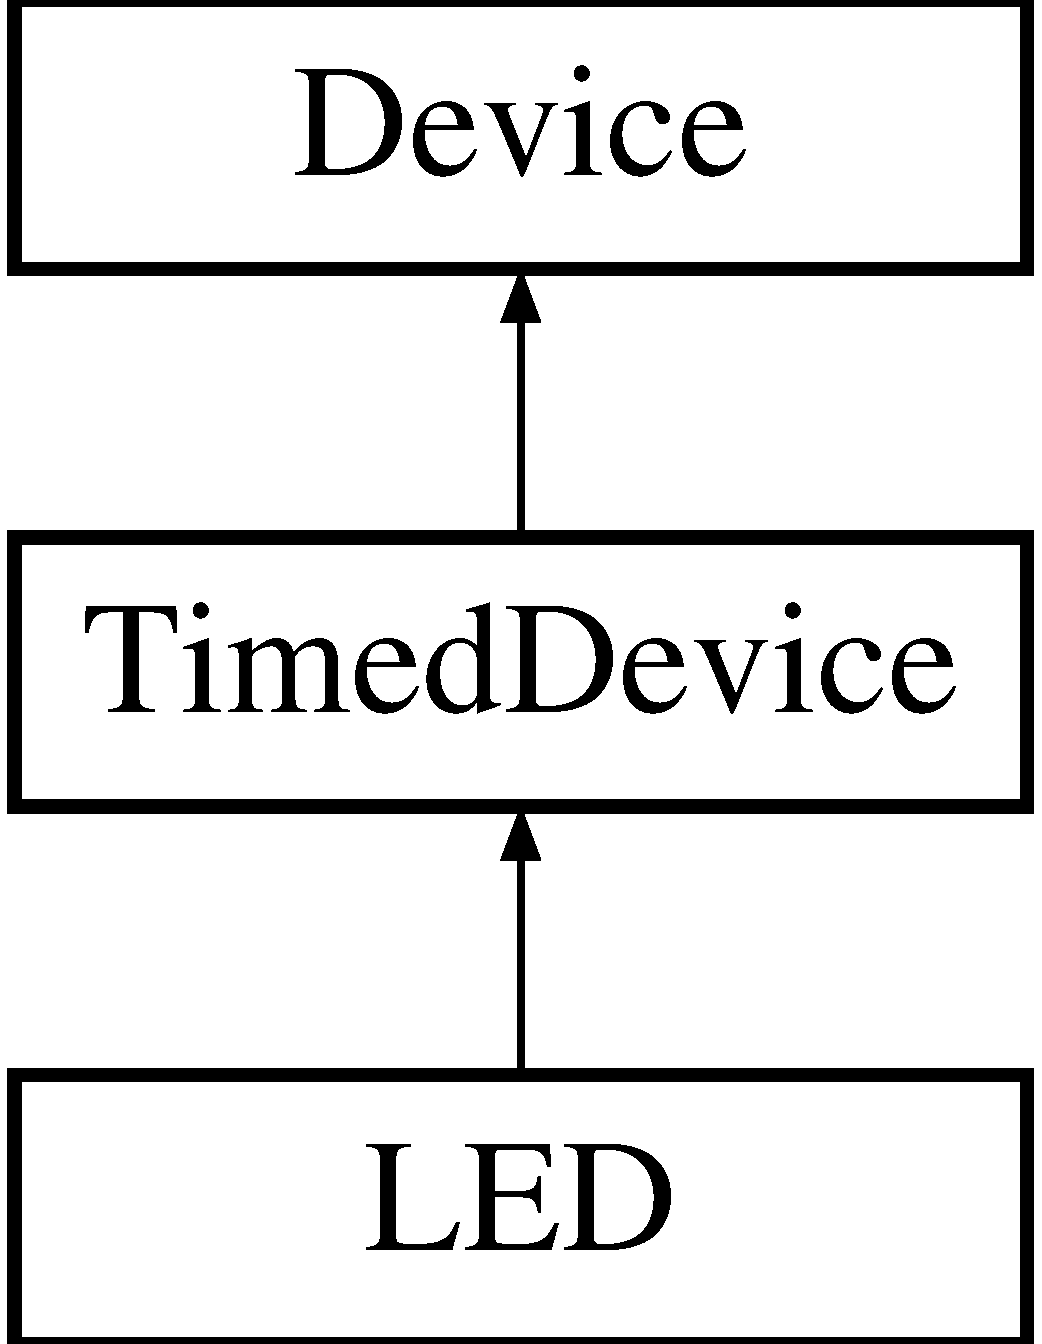
\includegraphics[height=3.000000cm]{classLED}
\end{center}
\end{figure}
\subsection*{Métodos Públicos}
\begin{DoxyCompactItemize}
\item 
\hyperlink{classLED_a4b8692dfdef842d0da59ac0644eb0e97}{L\-E\-D} (uint8\-\_\-t pin)
\item 
void \hyperlink{classLED_a62e402841c861af9bb4eb679f5afc7d6}{begin} ()
\begin{DoxyCompactList}\small\item\em Inicializa o dispositivo. \end{DoxyCompactList}\item 
void \hyperlink{classLED_a11f7b87c240eb671482a7af687b0737c}{stop} ()
\begin{DoxyCompactList}\small\item\em Interrompe o funcionamento do dispositivo. \end{DoxyCompactList}\item 
void \hyperlink{classLED_a8b85489d7bcfc54252f28abc0a5ba3cf}{reset} ()
\begin{DoxyCompactList}\small\item\em Redefine o estado do dispositivo. \end{DoxyCompactList}\item 
void \hyperlink{classLED_ad615d612f5b0c7dac4dde5245f191382}{update} ()
\begin{DoxyCompactList}\small\item\em Atualiza o estado atual do dispositivo. \end{DoxyCompactList}\item 
bool \hyperlink{classLED_a36cc9854b853baba06ee3d1e74339c6f}{is\-Ready} ()
\begin{DoxyCompactList}\small\item\em Verifica se o dispositivo está pronto para receber novos comandos ou leituras. \end{DoxyCompactList}\item 
uint8\-\_\-t \hyperlink{classLED_a70416944b6d3cae4a8dc73859a3df2aa}{get} (uint8\-\_\-t $\ast$buffer, uint8\-\_\-t size)
\item 
void \hyperlink{classLED_aae83a677cee4ee5cb952ccbb22e57781}{set} (const uint8\-\_\-t $\ast$data, uint8\-\_\-t size=1)
\item 
void \hyperlink{classLED_a126e67dbf18aae87b9e43daed89eb837}{set\-State} (uint8\-\_\-t state)
\item 
void \hyperlink{classLED_a27e6e12de55a23dc87644c0c28972e51}{toggle} ()
\item 
uint8\-\_\-t \hyperlink{classLED_ac2003f82c3aa7eafee2e95a790ca8549}{get\-State} ()
\item 
void \hyperlink{classLED_aae1edcf4dd4a353a867ae0043cf0a7c7}{blink} (uint16\-\_\-t period, uint8\-\_\-t times)
\item 
void \hyperlink{classLED_ab657582648d1b5f488d1a67e615a5e50}{set\-Period} (uint16\-\_\-t period)
\item 
uint16\-\_\-t \hyperlink{classLED_a02184f5f15fac9fd237d7a95d3e8b7ec}{get\-Period} ()
\item 
void \hyperlink{classLED_a3b3d64d836947492ef8f8320327b6674}{set\-Blink\-Times} (uint8\-\_\-t times)
\item 
uint8\-\_\-t \hyperlink{classLED_a017d73ffbe5db1159e7b7d4e4e8d5370}{get\-Blink\-Times} ()
\item 
void \hyperlink{classLED_ab63f595aca673a34fe0c9ae2d94349c1}{set\-P\-W\-M} (bool pwm)
\end{DoxyCompactItemize}
\subsection*{Additional Inherited Members}


\subsection{Construtores \& Destrutores}
\hypertarget{classLED_a4b8692dfdef842d0da59ac0644eb0e97}{\index{L\-E\-D@{L\-E\-D}!L\-E\-D@{L\-E\-D}}
\index{L\-E\-D@{L\-E\-D}!LED@{L\-E\-D}}
\subsubsection[{L\-E\-D}]{\setlength{\rightskip}{0pt plus 5cm}L\-E\-D\-::\-L\-E\-D (
\begin{DoxyParamCaption}
\item[{uint8\-\_\-t}]{pin}
\end{DoxyParamCaption}
)}}\label{classLED_a4b8692dfdef842d0da59ac0644eb0e97}


\subsection{Métodos}
\hypertarget{classLED_a62e402841c861af9bb4eb679f5afc7d6}{\index{L\-E\-D@{L\-E\-D}!begin@{begin}}
\index{begin@{begin}!LED@{L\-E\-D}}
\subsubsection[{begin}]{\setlength{\rightskip}{0pt plus 5cm}void L\-E\-D\-::begin (
\begin{DoxyParamCaption}
{}
\end{DoxyParamCaption}
)\hspace{0.3cm}{\ttfamily [virtual]}}}\label{classLED_a62e402841c861af9bb4eb679f5afc7d6}


Inicializa o dispositivo. 

Esta função é executada apenas uma vez em \hyperlink{classRobot_a6c7ee2437ae5427a19f2de4903ca0df9}{Robot\-::begin()}. 

Implementa \hyperlink{classDevice_a0dc99b16a220489d787a1cbcef4875d9}{Device}.

\hypertarget{classLED_aae1edcf4dd4a353a867ae0043cf0a7c7}{\index{L\-E\-D@{L\-E\-D}!blink@{blink}}
\index{blink@{blink}!LED@{L\-E\-D}}
\subsubsection[{blink}]{\setlength{\rightskip}{0pt plus 5cm}void L\-E\-D\-::blink (
\begin{DoxyParamCaption}
\item[{uint16\-\_\-t}]{period, }
\item[{uint8\-\_\-t}]{times}
\end{DoxyParamCaption}
)}}\label{classLED_aae1edcf4dd4a353a867ae0043cf0a7c7}
\hypertarget{classLED_a70416944b6d3cae4a8dc73859a3df2aa}{\index{L\-E\-D@{L\-E\-D}!get@{get}}
\index{get@{get}!LED@{L\-E\-D}}
\subsubsection[{get}]{\setlength{\rightskip}{0pt plus 5cm}uint8\-\_\-t L\-E\-D\-::get (
\begin{DoxyParamCaption}
\item[{uint8\-\_\-t $\ast$}]{buffer, }
\item[{uint8\-\_\-t}]{size}
\end{DoxyParamCaption}
)\hspace{0.3cm}{\ttfamily [virtual]}}}\label{classLED_a70416944b6d3cae4a8dc73859a3df2aa}

\begin{DoxyParams}[1]{Parâmetros}
\mbox{\tt out}  & {\em buffer} & Array de bytes com tamanho suficiente para armazenar a resposta. \\
\hline
 & {\em size} & Tamanho do {\ttfamily buffer}.\\
\hline
\end{DoxyParams}
\begin{DoxyReturn}{Retorna}
O numero de bytes escritos em {\ttfamily buffer}. 
\end{DoxyReturn}


Implementa \hyperlink{classDevice_a0057af09515609c289d5da3be19dcc8d}{Device}.

\hypertarget{classLED_a017d73ffbe5db1159e7b7d4e4e8d5370}{\index{L\-E\-D@{L\-E\-D}!get\-Blink\-Times@{get\-Blink\-Times}}
\index{get\-Blink\-Times@{get\-Blink\-Times}!LED@{L\-E\-D}}
\subsubsection[{get\-Blink\-Times}]{\setlength{\rightskip}{0pt plus 5cm}uint8\-\_\-t L\-E\-D\-::get\-Blink\-Times (
\begin{DoxyParamCaption}
{}
\end{DoxyParamCaption}
)}}\label{classLED_a017d73ffbe5db1159e7b7d4e4e8d5370}
\hypertarget{classLED_a02184f5f15fac9fd237d7a95d3e8b7ec}{\index{L\-E\-D@{L\-E\-D}!get\-Period@{get\-Period}}
\index{get\-Period@{get\-Period}!LED@{L\-E\-D}}
\subsubsection[{get\-Period}]{\setlength{\rightskip}{0pt plus 5cm}uint16\-\_\-t L\-E\-D\-::get\-Period (
\begin{DoxyParamCaption}
{}
\end{DoxyParamCaption}
)}}\label{classLED_a02184f5f15fac9fd237d7a95d3e8b7ec}
\hypertarget{classLED_ac2003f82c3aa7eafee2e95a790ca8549}{\index{L\-E\-D@{L\-E\-D}!get\-State@{get\-State}}
\index{get\-State@{get\-State}!LED@{L\-E\-D}}
\subsubsection[{get\-State}]{\setlength{\rightskip}{0pt plus 5cm}uint8\-\_\-t L\-E\-D\-::get\-State (
\begin{DoxyParamCaption}
{}
\end{DoxyParamCaption}
)}}\label{classLED_ac2003f82c3aa7eafee2e95a790ca8549}
\hypertarget{classLED_a36cc9854b853baba06ee3d1e74339c6f}{\index{L\-E\-D@{L\-E\-D}!is\-Ready@{is\-Ready}}
\index{is\-Ready@{is\-Ready}!LED@{L\-E\-D}}
\subsubsection[{is\-Ready}]{\setlength{\rightskip}{0pt plus 5cm}bool L\-E\-D\-::is\-Ready (
\begin{DoxyParamCaption}
{}
\end{DoxyParamCaption}
)\hspace{0.3cm}{\ttfamily [virtual]}}}\label{classLED_a36cc9854b853baba06ee3d1e74339c6f}


Verifica se o dispositivo está pronto para receber novos comandos ou leituras. 

É importante para \hyperlink{classRobot}{Robot} definir se uma ação de maior grau de abstração foi concluída ou não.

\begin{DoxyReturn}{Retorna}
{\ttfamily T\-R\-U\-E} se o dispositivo está ocioso. 
\end{DoxyReturn}


Implementa \hyperlink{classDevice_a30065df084d450dbaae9d68215e01e6f}{Device}.

\hypertarget{classLED_a8b85489d7bcfc54252f28abc0a5ba3cf}{\index{L\-E\-D@{L\-E\-D}!reset@{reset}}
\index{reset@{reset}!LED@{L\-E\-D}}
\subsubsection[{reset}]{\setlength{\rightskip}{0pt plus 5cm}void L\-E\-D\-::reset (
\begin{DoxyParamCaption}
{}
\end{DoxyParamCaption}
)\hspace{0.3cm}{\ttfamily [virtual]}}}\label{classLED_a8b85489d7bcfc54252f28abc0a5ba3cf}


Redefine o estado do dispositivo. 



Implementa \hyperlink{classDevice_a6e43162e890cb40eafb923b0c94d167a}{Device}.

\hypertarget{classLED_aae83a677cee4ee5cb952ccbb22e57781}{\index{L\-E\-D@{L\-E\-D}!set@{set}}
\index{set@{set}!LED@{L\-E\-D}}
\subsubsection[{set}]{\setlength{\rightskip}{0pt plus 5cm}void L\-E\-D\-::set (
\begin{DoxyParamCaption}
\item[{const uint8\-\_\-t $\ast$}]{data, }
\item[{uint8\-\_\-t}]{size = {\ttfamily 1}}
\end{DoxyParamCaption}
)\hspace{0.3cm}{\ttfamily [virtual]}}}\label{classLED_aae83a677cee4ee5cb952ccbb22e57781}

\begin{DoxyParams}[1]{Parâmetros}
\mbox{\tt in}  & {\em data} & Mensagem a ser processada pelo dispositivo. \\
\hline
 & {\em size} & Tamanho do vetor data. \\
\hline
\end{DoxyParams}


Implementa \hyperlink{classDevice_a3b4bf3ff761f93c024675548755586d8}{Device}.

\hypertarget{classLED_a3b3d64d836947492ef8f8320327b6674}{\index{L\-E\-D@{L\-E\-D}!set\-Blink\-Times@{set\-Blink\-Times}}
\index{set\-Blink\-Times@{set\-Blink\-Times}!LED@{L\-E\-D}}
\subsubsection[{set\-Blink\-Times}]{\setlength{\rightskip}{0pt plus 5cm}void L\-E\-D\-::set\-Blink\-Times (
\begin{DoxyParamCaption}
\item[{uint8\-\_\-t}]{times}
\end{DoxyParamCaption}
)}}\label{classLED_a3b3d64d836947492ef8f8320327b6674}
\hypertarget{classLED_ab657582648d1b5f488d1a67e615a5e50}{\index{L\-E\-D@{L\-E\-D}!set\-Period@{set\-Period}}
\index{set\-Period@{set\-Period}!LED@{L\-E\-D}}
\subsubsection[{set\-Period}]{\setlength{\rightskip}{0pt plus 5cm}void L\-E\-D\-::set\-Period (
\begin{DoxyParamCaption}
\item[{uint16\-\_\-t}]{period}
\end{DoxyParamCaption}
)}}\label{classLED_ab657582648d1b5f488d1a67e615a5e50}
\hypertarget{classLED_ab63f595aca673a34fe0c9ae2d94349c1}{\index{L\-E\-D@{L\-E\-D}!set\-P\-W\-M@{set\-P\-W\-M}}
\index{set\-P\-W\-M@{set\-P\-W\-M}!LED@{L\-E\-D}}
\subsubsection[{set\-P\-W\-M}]{\setlength{\rightskip}{0pt plus 5cm}void L\-E\-D\-::set\-P\-W\-M (
\begin{DoxyParamCaption}
\item[{bool}]{pwm}
\end{DoxyParamCaption}
)}}\label{classLED_ab63f595aca673a34fe0c9ae2d94349c1}
\hypertarget{classLED_a126e67dbf18aae87b9e43daed89eb837}{\index{L\-E\-D@{L\-E\-D}!set\-State@{set\-State}}
\index{set\-State@{set\-State}!LED@{L\-E\-D}}
\subsubsection[{set\-State}]{\setlength{\rightskip}{0pt plus 5cm}void L\-E\-D\-::set\-State (
\begin{DoxyParamCaption}
\item[{uint8\-\_\-t}]{state}
\end{DoxyParamCaption}
)}}\label{classLED_a126e67dbf18aae87b9e43daed89eb837}
\hypertarget{classLED_a11f7b87c240eb671482a7af687b0737c}{\index{L\-E\-D@{L\-E\-D}!stop@{stop}}
\index{stop@{stop}!LED@{L\-E\-D}}
\subsubsection[{stop}]{\setlength{\rightskip}{0pt plus 5cm}void L\-E\-D\-::stop (
\begin{DoxyParamCaption}
{}
\end{DoxyParamCaption}
)\hspace{0.3cm}{\ttfamily [virtual]}}}\label{classLED_a11f7b87c240eb671482a7af687b0737c}


Interrompe o funcionamento do dispositivo. 



Implementa \hyperlink{classDevice_a22430f274658b04c280b5cc2d53aa1e4}{Device}.

\hypertarget{classLED_a27e6e12de55a23dc87644c0c28972e51}{\index{L\-E\-D@{L\-E\-D}!toggle@{toggle}}
\index{toggle@{toggle}!LED@{L\-E\-D}}
\subsubsection[{toggle}]{\setlength{\rightskip}{0pt plus 5cm}void L\-E\-D\-::toggle (
\begin{DoxyParamCaption}
{}
\end{DoxyParamCaption}
)}}\label{classLED_a27e6e12de55a23dc87644c0c28972e51}
\hypertarget{classLED_ad615d612f5b0c7dac4dde5245f191382}{\index{L\-E\-D@{L\-E\-D}!update@{update}}
\index{update@{update}!LED@{L\-E\-D}}
\subsubsection[{update}]{\setlength{\rightskip}{0pt plus 5cm}void L\-E\-D\-::update (
\begin{DoxyParamCaption}
{}
\end{DoxyParamCaption}
)\hspace{0.3cm}{\ttfamily [virtual]}}}\label{classLED_ad615d612f5b0c7dac4dde5245f191382}


Atualiza o estado atual do dispositivo. 

Esta função é executada uma vez a cada \hyperlink{classRobot_aa50d73cd1109a70133af442674ed3a1a}{Robot\-::step()}. 

Implementa \hyperlink{classDevice_a7e5226b6341b1cf2ec04a5913b97becc}{Device}.



A documentação para esta classe foi gerada a partir dos seguintes arquivos\-:\begin{DoxyCompactItemize}
\item 
\hyperlink{LED_8h}{L\-E\-D.\-h}\item 
\hyperlink{LED_8cpp}{L\-E\-D.\-cpp}\end{DoxyCompactItemize}

\hypertarget{classQuickRobot}{\section{Referência da Classe Quick\-Robot}
\label{classQuickRobot}\index{Quick\-Robot@{Quick\-Robot}}
}


A classe \hyperlink{classQuickRobot}{Quick\-Robot}.  




{\ttfamily \#include $<$Robot.\-h$>$}

Diagrama de Hierarquia para Quick\-Robot\-:\begin{figure}[H]
\begin{center}
\leavevmode
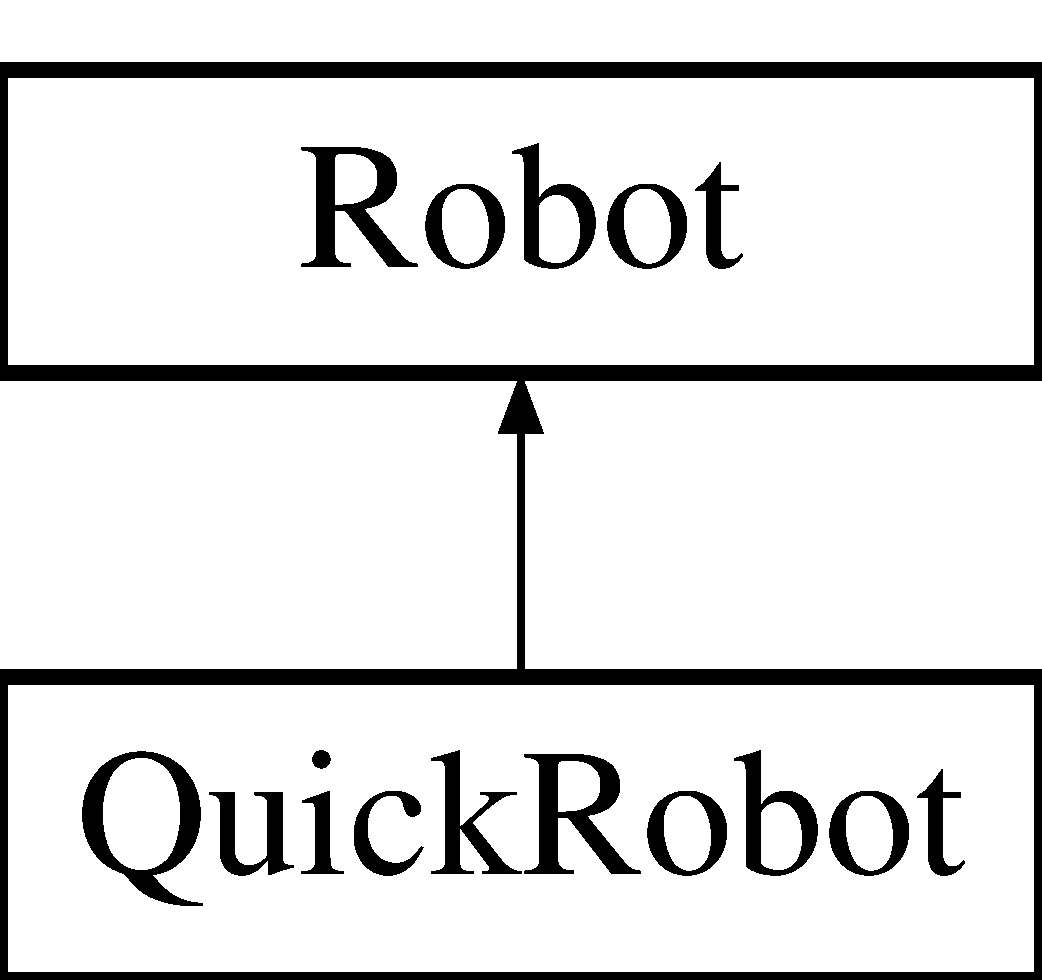
\includegraphics[height=2.000000cm]{classQuickRobot}
\end{center}
\end{figure}
\subsection*{Métodos Públicos}
\begin{DoxyCompactItemize}
\item 
\hyperlink{classQuickRobot_ab43c04a584a584f332119137f0b51c43}{Quick\-Robot} (void($\ast$\hyperlink{classQuickRobot_a936a04970e2fe8694256a70816b697f6}{think})(), void($\ast$dev\-Ready)(\hyperlink{classDevice}{Device} \&d), void($\ast$msg\-Rec)(const uint8\-\_\-t $\ast$, uint8\-\_\-t, \hyperlink{classConnection}{Connection} \&))
\item 
void \hyperlink{classQuickRobot_a936a04970e2fe8694256a70816b697f6}{think} ()
\begin{DoxyCompactList}\small\item\em Função responsável por tomar novas decisões com base nos sensores e atuadores do robô, em um determinado ciclo. \end{DoxyCompactList}\item 
void \hyperlink{classQuickRobot_a95d490eb2e580d362b99eb6c90927256}{device\-Ready} (\hyperlink{classDevice}{Device} \&d)
\begin{DoxyCompactList}\small\item\em Função executada quando um dispositivo anteriormente ocupado torna-\/se disponível. \end{DoxyCompactList}\item 
void \hyperlink{classQuickRobot_a96eda0e5288726364f4a02ef7912e21b}{message\-Received} (const uint8\-\_\-t $\ast$data, uint8\-\_\-t size, \hyperlink{classConnection}{Connection} \&connection)
\begin{DoxyCompactList}\small\item\em Função executada quando uma mensagem é recebida por alguma conexão. \end{DoxyCompactList}\end{DoxyCompactItemize}
\subsection*{Additional Inherited Members}


\subsection{Descrição Detalhada}
A classe \hyperlink{classQuickRobot}{Quick\-Robot}. 

\subsection{Construtores \& Destrutores}
\hypertarget{classQuickRobot_ab43c04a584a584f332119137f0b51c43}{\index{Quick\-Robot@{Quick\-Robot}!Quick\-Robot@{Quick\-Robot}}
\index{Quick\-Robot@{Quick\-Robot}!QuickRobot@{Quick\-Robot}}
\subsubsection[{Quick\-Robot}]{\setlength{\rightskip}{0pt plus 5cm}Quick\-Robot\-::\-Quick\-Robot (
\begin{DoxyParamCaption}
\item[{void($\ast$)()}]{think, }
\item[{void($\ast$)({\bf Device} \&d)}]{dev\-Ready, }
\item[{void($\ast$)(const uint8\-\_\-t $\ast$, uint8\-\_\-t, {\bf Connection} \&)}]{msg\-Rec}
\end{DoxyParamCaption}
)\hspace{0.3cm}{\ttfamily [inline]}}}\label{classQuickRobot_ab43c04a584a584f332119137f0b51c43}


\subsection{Métodos}
\hypertarget{classQuickRobot_a95d490eb2e580d362b99eb6c90927256}{\index{Quick\-Robot@{Quick\-Robot}!device\-Ready@{device\-Ready}}
\index{device\-Ready@{device\-Ready}!QuickRobot@{Quick\-Robot}}
\subsubsection[{device\-Ready}]{\setlength{\rightskip}{0pt plus 5cm}void Quick\-Robot\-::device\-Ready (
\begin{DoxyParamCaption}
\item[{{\bf Device} \&}]{d}
\end{DoxyParamCaption}
)\hspace{0.3cm}{\ttfamily [inline]}, {\ttfamily [virtual]}}}\label{classQuickRobot_a95d490eb2e580d362b99eb6c90927256}


Função executada quando um dispositivo anteriormente ocupado torna-\/se disponível. 


\begin{DoxyParams}{Parâmetros}
{\em d} & Referência ao dispositivo em questão. \\
\hline
\end{DoxyParams}


Implementa \hyperlink{classRobot_aaa0c932d862aed7556b068ebb70a917a}{Robot}.

\hypertarget{classQuickRobot_a96eda0e5288726364f4a02ef7912e21b}{\index{Quick\-Robot@{Quick\-Robot}!message\-Received@{message\-Received}}
\index{message\-Received@{message\-Received}!QuickRobot@{Quick\-Robot}}
\subsubsection[{message\-Received}]{\setlength{\rightskip}{0pt plus 5cm}void Quick\-Robot\-::message\-Received (
\begin{DoxyParamCaption}
\item[{const uint8\-\_\-t $\ast$}]{data, }
\item[{uint8\-\_\-t}]{size, }
\item[{{\bf Connection} \&}]{connection}
\end{DoxyParamCaption}
)\hspace{0.3cm}{\ttfamily [inline]}, {\ttfamily [virtual]}}}\label{classQuickRobot_a96eda0e5288726364f4a02ef7912e21b}


Função executada quando uma mensagem é recebida por alguma conexão. 


\begin{DoxyParams}[1]{Parâmetros}
\mbox{\tt in}  & {\em data} & Um vetor de constantes de 8bits (byte) contendo a mensagem. \\
\hline
 & {\em size} & O tamanho da mensagem em bytes. \\
\hline
 & {\em connection} & O I\-D da conexão que recebeu a mensagem. \\
\hline
\end{DoxyParams}


Implementa \hyperlink{classRobot_ab02c09bdea244d38bcfd0010b9554b6f}{Robot}.

\hypertarget{classQuickRobot_a936a04970e2fe8694256a70816b697f6}{\index{Quick\-Robot@{Quick\-Robot}!think@{think}}
\index{think@{think}!QuickRobot@{Quick\-Robot}}
\subsubsection[{think}]{\setlength{\rightskip}{0pt plus 5cm}void Quick\-Robot\-::think (
\begin{DoxyParamCaption}
{}
\end{DoxyParamCaption}
)\hspace{0.3cm}{\ttfamily [inline]}, {\ttfamily [virtual]}}}\label{classQuickRobot_a936a04970e2fe8694256a70816b697f6}


Função responsável por tomar novas decisões com base nos sensores e atuadores do robô, em um determinado ciclo. 

É executada uma vez a cada \hyperlink{classRobot_aa50d73cd1109a70133af442674ed3a1a}{Robot\-::step()}. 

Implementa \hyperlink{classRobot_a75cfdd8e35e007abe24ffae66a8ecf1d}{Robot}.



A documentação para esta classe foi gerada a partir do seguinte arquivo\-:\begin{DoxyCompactItemize}
\item 
\hyperlink{Robot_8h}{Robot.\-h}\end{DoxyCompactItemize}

\hypertarget{classRadioConnection}{\section{Referência da Classe Radio\-Connection}
\label{classRadioConnection}\index{Radio\-Connection@{Radio\-Connection}}
}


{\ttfamily \#include $<$Radio\-Connection.\-h$>$}

Diagrama de Hierarquia para Radio\-Connection\-:\begin{figure}[H]
\begin{center}
\leavevmode
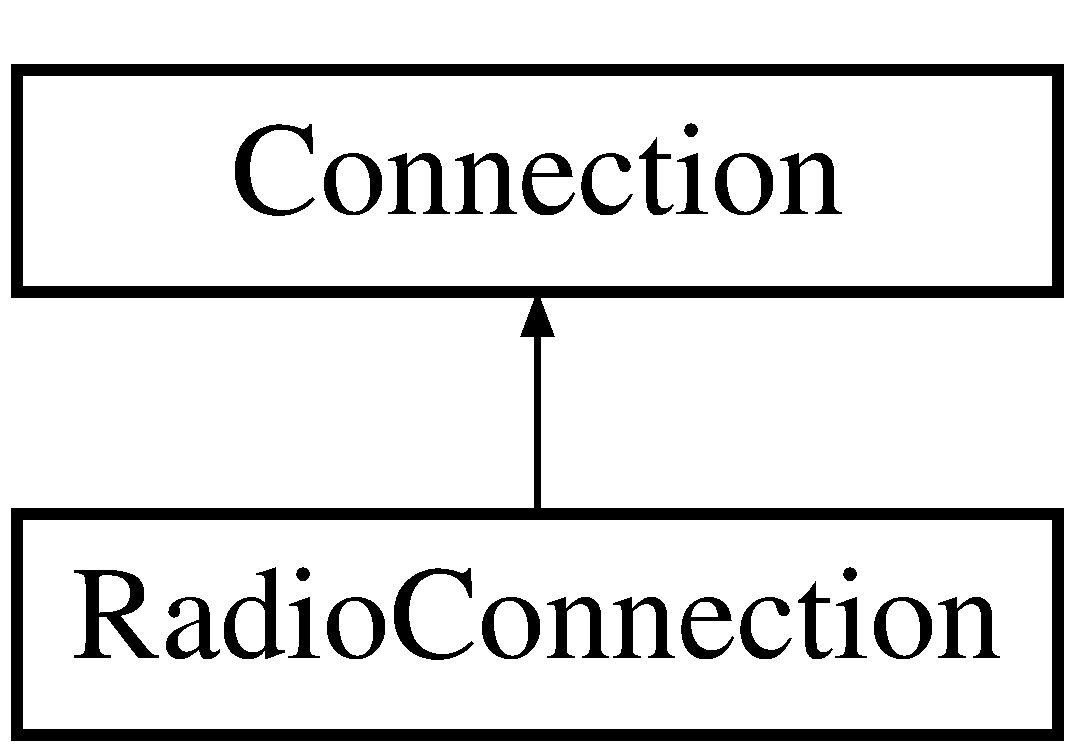
\includegraphics[height=2.000000cm]{classRadioConnection}
\end{center}
\end{figure}
\subsection*{Métodos Públicos}
\begin{DoxyCompactItemize}
\item 
\hyperlink{classRadioConnection_ab901c79237a74d39f756b497140c9256}{Radio\-Connection} (uint8\-\_\-t pin, uint8\-\_\-t S\-P\-I\-\_\-\-S\-S, bool \hyperlink{classRadioConnection_a1e47d7b5f29f786ff2c90bf7446ac145}{is\-Master}=false)
\item 
bool \hyperlink{classRadioConnection_a1e47d7b5f29f786ff2c90bf7446ac145}{is\-Master} ()
\item 
void \hyperlink{classRadioConnection_a1deb37d098b17cfdf2c5c90e67a279aa}{begin} ()
\begin{DoxyCompactList}\small\item\em Inicializa a conexão. \end{DoxyCompactList}\item 
void \hyperlink{classRadioConnection_a50c54a480bbb37df2ecefb82aa9aa2a9}{start} ()
\item 
void \hyperlink{classRadioConnection_aa351758992987f76f2f14700c35daf04}{stop} ()
\item 
void \hyperlink{classRadioConnection_a170cffba8c7b427948429b41e6014ea3}{print\-Details} ()
\item 
uint8\-\_\-t \hyperlink{classRadioConnection_a970ffcf382ae789c22023857c5c48d83}{available} ()
\begin{DoxyCompactList}\small\item\em Verifica se existe alguma mensagem disponivel. \end{DoxyCompactList}\item 
uint8\-\_\-t \hyperlink{classRadioConnection_a6dc7c7b2a7c9b5d754d73f80516a37fc}{receive\-Message} (uint8\-\_\-t $\ast$buffer, uint8\-\_\-t size)
\begin{DoxyCompactList}\small\item\em Recebe uma mensagem. \end{DoxyCompactList}\item 
bool \hyperlink{classRadioConnection_a1bc09119403b84463264710ea40f5a4c}{send\-Message} (const uint8\-\_\-t $\ast$data, uint8\-\_\-t size)
\begin{DoxyCompactList}\small\item\em Envia uma mensagem. \end{DoxyCompactList}\end{DoxyCompactItemize}


\subsection{Construtores \& Destrutores}
\hypertarget{classRadioConnection_ab901c79237a74d39f756b497140c9256}{\index{Radio\-Connection@{Radio\-Connection}!Radio\-Connection@{Radio\-Connection}}
\index{Radio\-Connection@{Radio\-Connection}!RadioConnection@{Radio\-Connection}}
\subsubsection[{Radio\-Connection}]{\setlength{\rightskip}{0pt plus 5cm}Radio\-Connection\-::\-Radio\-Connection (
\begin{DoxyParamCaption}
\item[{uint8\-\_\-t}]{pin, }
\item[{uint8\-\_\-t}]{S\-P\-I\-\_\-\-S\-S, }
\item[{bool}]{is\-Master = {\ttfamily false}}
\end{DoxyParamCaption}
)}}\label{classRadioConnection_ab901c79237a74d39f756b497140c9256}


\subsection{Métodos}
\hypertarget{classRadioConnection_a970ffcf382ae789c22023857c5c48d83}{\index{Radio\-Connection@{Radio\-Connection}!available@{available}}
\index{available@{available}!RadioConnection@{Radio\-Connection}}
\subsubsection[{available}]{\setlength{\rightskip}{0pt plus 5cm}uint8\-\_\-t Radio\-Connection\-::available (
\begin{DoxyParamCaption}
{}
\end{DoxyParamCaption}
)\hspace{0.3cm}{\ttfamily [virtual]}}}\label{classRadioConnection_a970ffcf382ae789c22023857c5c48d83}


Verifica se existe alguma mensagem disponivel. 

\begin{DoxyReturn}{Retorna}
O numero de bytes disponiveis, se possivel. 
\end{DoxyReturn}


Implementa \hyperlink{classConnection_acd5ee426481b2aca2903d96f6f807341}{Connection}.

\hypertarget{classRadioConnection_a1deb37d098b17cfdf2c5c90e67a279aa}{\index{Radio\-Connection@{Radio\-Connection}!begin@{begin}}
\index{begin@{begin}!RadioConnection@{Radio\-Connection}}
\subsubsection[{begin}]{\setlength{\rightskip}{0pt plus 5cm}void Radio\-Connection\-::begin (
\begin{DoxyParamCaption}
{}
\end{DoxyParamCaption}
)\hspace{0.3cm}{\ttfamily [virtual]}}}\label{classRadioConnection_a1deb37d098b17cfdf2c5c90e67a279aa}


Inicializa a conexão. 



Implementa \hyperlink{classConnection_a2e5c7e67928fac5fea45e56c11d1ed31}{Connection}.

\hypertarget{classRadioConnection_a1e47d7b5f29f786ff2c90bf7446ac145}{\index{Radio\-Connection@{Radio\-Connection}!is\-Master@{is\-Master}}
\index{is\-Master@{is\-Master}!RadioConnection@{Radio\-Connection}}
\subsubsection[{is\-Master}]{\setlength{\rightskip}{0pt plus 5cm}bool Radio\-Connection\-::is\-Master (
\begin{DoxyParamCaption}
{}
\end{DoxyParamCaption}
)}}\label{classRadioConnection_a1e47d7b5f29f786ff2c90bf7446ac145}
\hypertarget{classRadioConnection_a170cffba8c7b427948429b41e6014ea3}{\index{Radio\-Connection@{Radio\-Connection}!print\-Details@{print\-Details}}
\index{print\-Details@{print\-Details}!RadioConnection@{Radio\-Connection}}
\subsubsection[{print\-Details}]{\setlength{\rightskip}{0pt plus 5cm}void Radio\-Connection\-::print\-Details (
\begin{DoxyParamCaption}
{}
\end{DoxyParamCaption}
)}}\label{classRadioConnection_a170cffba8c7b427948429b41e6014ea3}
\hypertarget{classRadioConnection_a6dc7c7b2a7c9b5d754d73f80516a37fc}{\index{Radio\-Connection@{Radio\-Connection}!receive\-Message@{receive\-Message}}
\index{receive\-Message@{receive\-Message}!RadioConnection@{Radio\-Connection}}
\subsubsection[{receive\-Message}]{\setlength{\rightskip}{0pt plus 5cm}uint8\-\_\-t Radio\-Connection\-::receive\-Message (
\begin{DoxyParamCaption}
\item[{uint8\-\_\-t $\ast$}]{buffer, }
\item[{uint8\-\_\-t}]{size}
\end{DoxyParamCaption}
)\hspace{0.3cm}{\ttfamily [virtual]}}}\label{classRadioConnection_a6dc7c7b2a7c9b5d754d73f80516a37fc}


Recebe uma mensagem. 


\begin{DoxyParams}[1]{Parâmetros}
\mbox{\tt out}  & {\em buffer} & Um array de bytes usado para armazenar a mensagem recebida. \\
\hline
 & {\em size} & O tamanho do {\ttfamily buffer}.\\
\hline
\end{DoxyParams}
\begin{DoxyReturn}{Retorna}
O tamanho da mensagem recebida. 
\end{DoxyReturn}


Implementa \hyperlink{classConnection_a315961bc8327f38e4f4e09b832fc60a1}{Connection}.

\hypertarget{classRadioConnection_a1bc09119403b84463264710ea40f5a4c}{\index{Radio\-Connection@{Radio\-Connection}!send\-Message@{send\-Message}}
\index{send\-Message@{send\-Message}!RadioConnection@{Radio\-Connection}}
\subsubsection[{send\-Message}]{\setlength{\rightskip}{0pt plus 5cm}bool Radio\-Connection\-::send\-Message (
\begin{DoxyParamCaption}
\item[{const uint8\-\_\-t $\ast$}]{data, }
\item[{uint8\-\_\-t}]{size}
\end{DoxyParamCaption}
)\hspace{0.3cm}{\ttfamily [virtual]}}}\label{classRadioConnection_a1bc09119403b84463264710ea40f5a4c}


Envia uma mensagem. 


\begin{DoxyParams}[1]{Parâmetros}
\mbox{\tt in}  & {\em data} & Um array de bytes contendo a mensagem. \\
\hline
 & {\em size} & O tamanho do array {\ttfamily data}.\\
\hline
\end{DoxyParams}
\begin{DoxyReturn}{Retorna}
{\ttfamily T\-R\-U\-E} se a mensagem foi entregue corretamente. 
\end{DoxyReturn}


Implementa \hyperlink{classConnection_aa03e632ed6b812d915fd40dccd18a080}{Connection}.

\hypertarget{classRadioConnection_a50c54a480bbb37df2ecefb82aa9aa2a9}{\index{Radio\-Connection@{Radio\-Connection}!start@{start}}
\index{start@{start}!RadioConnection@{Radio\-Connection}}
\subsubsection[{start}]{\setlength{\rightskip}{0pt plus 5cm}void Radio\-Connection\-::start (
\begin{DoxyParamCaption}
{}
\end{DoxyParamCaption}
)}}\label{classRadioConnection_a50c54a480bbb37df2ecefb82aa9aa2a9}
\hypertarget{classRadioConnection_aa351758992987f76f2f14700c35daf04}{\index{Radio\-Connection@{Radio\-Connection}!stop@{stop}}
\index{stop@{stop}!RadioConnection@{Radio\-Connection}}
\subsubsection[{stop}]{\setlength{\rightskip}{0pt plus 5cm}void Radio\-Connection\-::stop (
\begin{DoxyParamCaption}
{}
\end{DoxyParamCaption}
)}}\label{classRadioConnection_aa351758992987f76f2f14700c35daf04}


A documentação para esta classe foi gerada a partir dos seguintes arquivos\-:\begin{DoxyCompactItemize}
\item 
\hyperlink{RadioConnection_8h}{Radio\-Connection.\-h}\item 
\hyperlink{RadioConnection_8cpp}{Radio\-Connection.\-cpp}\end{DoxyCompactItemize}

\hypertarget{classRadioConnectionM}{\section{Referência da Classe Radio\-Connection\-M}
\label{classRadioConnectionM}\index{Radio\-Connection\-M@{Radio\-Connection\-M}}
}


{\ttfamily \#include $<$Radio\-Connection\-M.\-h$>$}

Diagrama de Hierarquia para Radio\-Connection\-M\-:\begin{figure}[H]
\begin{center}
\leavevmode
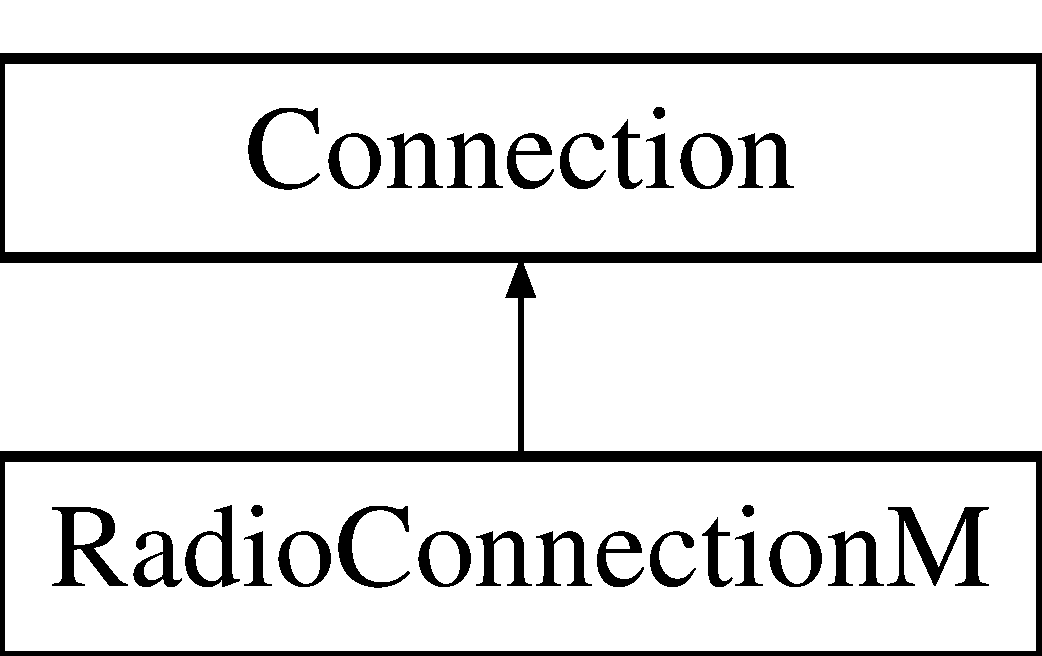
\includegraphics[height=2.000000cm]{classRadioConnectionM}
\end{center}
\end{figure}
\subsection*{Métodos Públicos}
\begin{DoxyCompactItemize}
\item 
\hyperlink{classRadioConnectionM_af147210568643b306924569d784fd5f1}{Radio\-Connection\-M} (uint8\-\_\-t pin, uint8\-\_\-t S\-P\-I\-\_\-\-S\-S, bool \hyperlink{classRadioConnectionM_a1db28139196c1f2fe17695f999dc3546}{is\-Master}=false)
\item 
bool \hyperlink{classRadioConnectionM_a1db28139196c1f2fe17695f999dc3546}{is\-Master} ()
\item 
void \hyperlink{classRadioConnectionM_acbfe7d993586efe2681e8fc07dcda463}{begin} ()
\begin{DoxyCompactList}\small\item\em Inicializa a conexão. \end{DoxyCompactList}\item 
void \hyperlink{classRadioConnectionM_a5486c1bcdd27afcf2e9dc5cccfd08660}{start} ()
\item 
void \hyperlink{classRadioConnectionM_a0deea36b1ed4dff4ce046bd008cb0da3}{stop} ()
\item 
uint8\-\_\-t \hyperlink{classRadioConnectionM_adfdbc2eb940e3a2a3798a76f02ea048a}{available} ()
\begin{DoxyCompactList}\small\item\em Verifica se existe alguma mensagem disponivel. \end{DoxyCompactList}\item 
bool \hyperlink{classRadioConnectionM_a8a4b19506bf383a0426023bef888e5a5}{send\-Message} (const uint8\-\_\-t $\ast$data, uint8\-\_\-t size)
\begin{DoxyCompactList}\small\item\em Envia uma mensagem. \end{DoxyCompactList}\item 
uint8\-\_\-t \hyperlink{classRadioConnectionM_a28ee1d2377f4d280723ce679b9f3db39}{receive\-Message} (uint8\-\_\-t $\ast$buffer, uint8\-\_\-t size)
\begin{DoxyCompactList}\small\item\em Recebe uma mensagem. \end{DoxyCompactList}\end{DoxyCompactItemize}


\subsection{Construtores \& Destrutores}
\hypertarget{classRadioConnectionM_af147210568643b306924569d784fd5f1}{\index{Radio\-Connection\-M@{Radio\-Connection\-M}!Radio\-Connection\-M@{Radio\-Connection\-M}}
\index{Radio\-Connection\-M@{Radio\-Connection\-M}!RadioConnectionM@{Radio\-Connection\-M}}
\subsubsection[{Radio\-Connection\-M}]{\setlength{\rightskip}{0pt plus 5cm}Radio\-Connection\-M\-::\-Radio\-Connection\-M (
\begin{DoxyParamCaption}
\item[{uint8\-\_\-t}]{pin, }
\item[{uint8\-\_\-t}]{S\-P\-I\-\_\-\-S\-S, }
\item[{bool}]{is\-Master = {\ttfamily false}}
\end{DoxyParamCaption}
)}}\label{classRadioConnectionM_af147210568643b306924569d784fd5f1}


\subsection{Métodos}
\hypertarget{classRadioConnectionM_adfdbc2eb940e3a2a3798a76f02ea048a}{\index{Radio\-Connection\-M@{Radio\-Connection\-M}!available@{available}}
\index{available@{available}!RadioConnectionM@{Radio\-Connection\-M}}
\subsubsection[{available}]{\setlength{\rightskip}{0pt plus 5cm}uint8\-\_\-t Radio\-Connection\-M\-::available (
\begin{DoxyParamCaption}
{}
\end{DoxyParamCaption}
)\hspace{0.3cm}{\ttfamily [virtual]}}}\label{classRadioConnectionM_adfdbc2eb940e3a2a3798a76f02ea048a}


Verifica se existe alguma mensagem disponivel. 

\begin{DoxyReturn}{Retorna}
O numero de bytes disponiveis, se possivel. 
\end{DoxyReturn}


Implementa \hyperlink{classConnection_acd5ee426481b2aca2903d96f6f807341}{Connection}.

\hypertarget{classRadioConnectionM_acbfe7d993586efe2681e8fc07dcda463}{\index{Radio\-Connection\-M@{Radio\-Connection\-M}!begin@{begin}}
\index{begin@{begin}!RadioConnectionM@{Radio\-Connection\-M}}
\subsubsection[{begin}]{\setlength{\rightskip}{0pt plus 5cm}void Radio\-Connection\-M\-::begin (
\begin{DoxyParamCaption}
{}
\end{DoxyParamCaption}
)\hspace{0.3cm}{\ttfamily [virtual]}}}\label{classRadioConnectionM_acbfe7d993586efe2681e8fc07dcda463}


Inicializa a conexão. 



Implementa \hyperlink{classConnection_a2e5c7e67928fac5fea45e56c11d1ed31}{Connection}.

\hypertarget{classRadioConnectionM_a1db28139196c1f2fe17695f999dc3546}{\index{Radio\-Connection\-M@{Radio\-Connection\-M}!is\-Master@{is\-Master}}
\index{is\-Master@{is\-Master}!RadioConnectionM@{Radio\-Connection\-M}}
\subsubsection[{is\-Master}]{\setlength{\rightskip}{0pt plus 5cm}bool Radio\-Connection\-M\-::is\-Master (
\begin{DoxyParamCaption}
{}
\end{DoxyParamCaption}
)}}\label{classRadioConnectionM_a1db28139196c1f2fe17695f999dc3546}
\hypertarget{classRadioConnectionM_a28ee1d2377f4d280723ce679b9f3db39}{\index{Radio\-Connection\-M@{Radio\-Connection\-M}!receive\-Message@{receive\-Message}}
\index{receive\-Message@{receive\-Message}!RadioConnectionM@{Radio\-Connection\-M}}
\subsubsection[{receive\-Message}]{\setlength{\rightskip}{0pt plus 5cm}uint8\-\_\-t Radio\-Connection\-M\-::receive\-Message (
\begin{DoxyParamCaption}
\item[{uint8\-\_\-t $\ast$}]{buffer, }
\item[{uint8\-\_\-t}]{size}
\end{DoxyParamCaption}
)\hspace{0.3cm}{\ttfamily [virtual]}}}\label{classRadioConnectionM_a28ee1d2377f4d280723ce679b9f3db39}


Recebe uma mensagem. 


\begin{DoxyParams}[1]{Parâmetros}
\mbox{\tt out}  & {\em buffer} & Um array de bytes usado para armazenar a mensagem recebida. \\
\hline
 & {\em size} & O tamanho do {\ttfamily buffer}.\\
\hline
\end{DoxyParams}
\begin{DoxyReturn}{Retorna}
O tamanho da mensagem recebida. 
\end{DoxyReturn}


Implementa \hyperlink{classConnection_a315961bc8327f38e4f4e09b832fc60a1}{Connection}.

\hypertarget{classRadioConnectionM_a8a4b19506bf383a0426023bef888e5a5}{\index{Radio\-Connection\-M@{Radio\-Connection\-M}!send\-Message@{send\-Message}}
\index{send\-Message@{send\-Message}!RadioConnectionM@{Radio\-Connection\-M}}
\subsubsection[{send\-Message}]{\setlength{\rightskip}{0pt plus 5cm}bool Radio\-Connection\-M\-::send\-Message (
\begin{DoxyParamCaption}
\item[{const uint8\-\_\-t $\ast$}]{data, }
\item[{uint8\-\_\-t}]{size}
\end{DoxyParamCaption}
)\hspace{0.3cm}{\ttfamily [virtual]}}}\label{classRadioConnectionM_a8a4b19506bf383a0426023bef888e5a5}


Envia uma mensagem. 


\begin{DoxyParams}[1]{Parâmetros}
\mbox{\tt in}  & {\em data} & Um array de bytes contendo a mensagem. \\
\hline
 & {\em size} & O tamanho do array {\ttfamily data}.\\
\hline
\end{DoxyParams}
\begin{DoxyReturn}{Retorna}
{\ttfamily T\-R\-U\-E} se a mensagem foi entregue corretamente. 
\end{DoxyReturn}


Implementa \hyperlink{classConnection_aa03e632ed6b812d915fd40dccd18a080}{Connection}.

\hypertarget{classRadioConnectionM_a5486c1bcdd27afcf2e9dc5cccfd08660}{\index{Radio\-Connection\-M@{Radio\-Connection\-M}!start@{start}}
\index{start@{start}!RadioConnectionM@{Radio\-Connection\-M}}
\subsubsection[{start}]{\setlength{\rightskip}{0pt plus 5cm}void Radio\-Connection\-M\-::start (
\begin{DoxyParamCaption}
{}
\end{DoxyParamCaption}
)}}\label{classRadioConnectionM_a5486c1bcdd27afcf2e9dc5cccfd08660}
\hypertarget{classRadioConnectionM_a0deea36b1ed4dff4ce046bd008cb0da3}{\index{Radio\-Connection\-M@{Radio\-Connection\-M}!stop@{stop}}
\index{stop@{stop}!RadioConnectionM@{Radio\-Connection\-M}}
\subsubsection[{stop}]{\setlength{\rightskip}{0pt plus 5cm}void Radio\-Connection\-M\-::stop (
\begin{DoxyParamCaption}
{}
\end{DoxyParamCaption}
)}}\label{classRadioConnectionM_a0deea36b1ed4dff4ce046bd008cb0da3}


A documentação para esta classe foi gerada a partir dos seguintes arquivos\-:\begin{DoxyCompactItemize}
\item 
\hyperlink{RadioConnectionM_8h}{Radio\-Connection\-M.\-h}\item 
\hyperlink{RadioConnectionM_8cpp}{Radio\-Connection\-M.\-cpp}\end{DoxyCompactItemize}

\hypertarget{classRadioRobot}{\section{Referência da Classe Radio\-Robot}
\label{classRadioRobot}\index{Radio\-Robot@{Radio\-Robot}}
}


{\ttfamily \#include $<$Radio\-Robot.\-h$>$}

Diagrama de Hierarquia para Radio\-Robot\-:\begin{figure}[H]
\begin{center}
\leavevmode
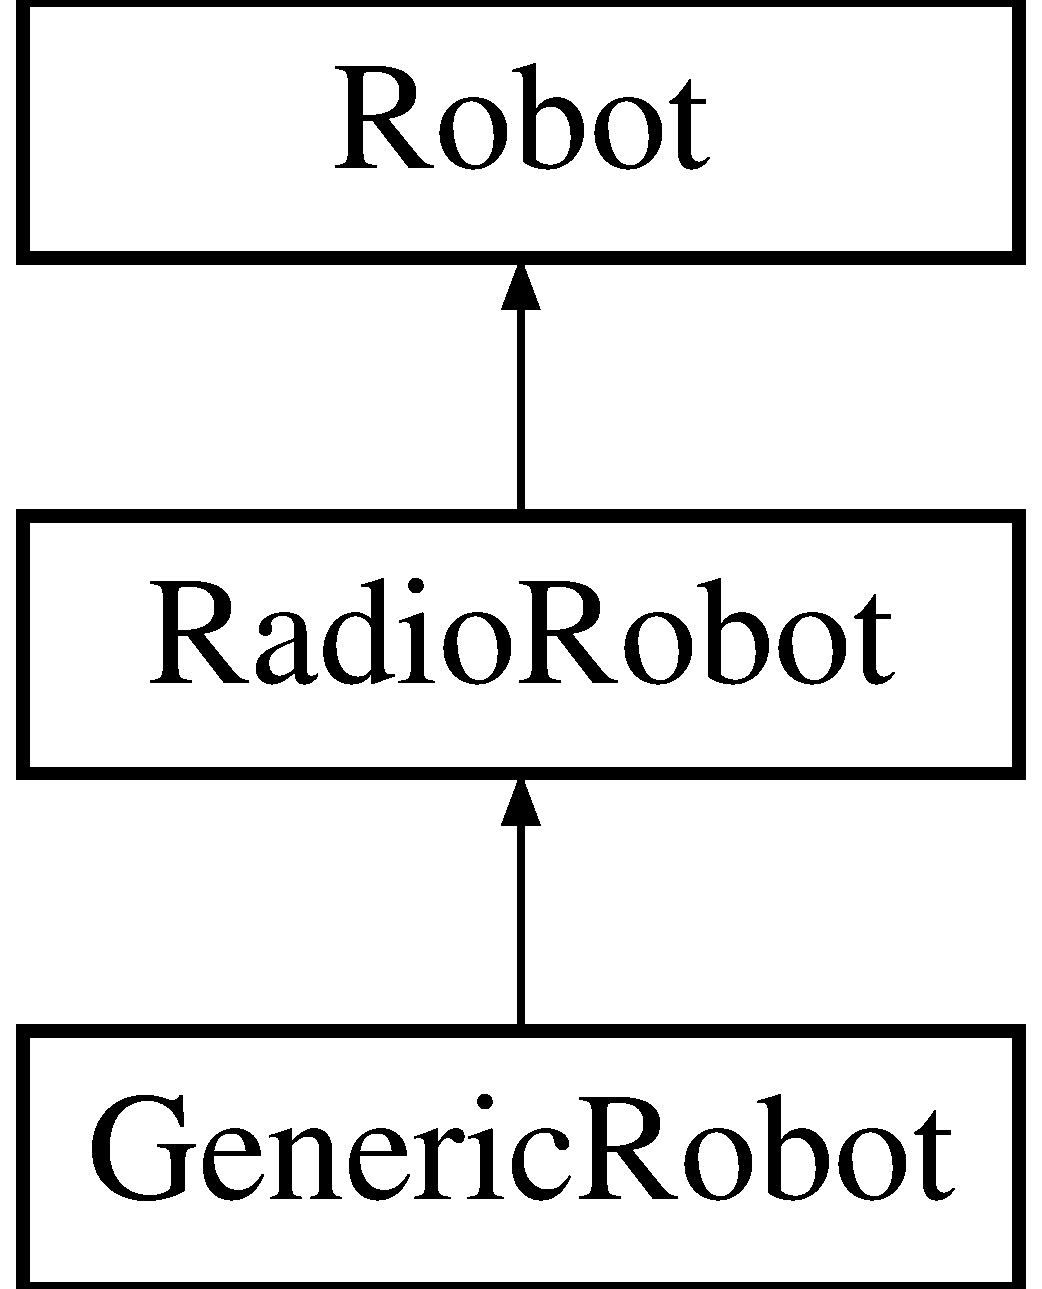
\includegraphics[height=3.000000cm]{classRadioRobot}
\end{center}
\end{figure}
\subsection*{Métodos Públicos}
\begin{DoxyCompactItemize}
\item 
\hyperlink{classRadioRobot_ad28a59e73e546d15004efda03525c143}{Radio\-Robot} ()
\item 
void \hyperlink{classRadioRobot_a1470b91c7a534545bdc6126c3065d4b8}{add\-Action} (\hyperlink{RadioRobot_8h_a3541f6ba20932adb767c7e0d8bdc6940}{Action\-Func} action)
\item 
void \hyperlink{classRadioRobot_a5de90c99faa941df35898349b6b148b5}{message\-Received} (const uint8\-\_\-t $\ast$data, uint8\-\_\-t size, \hyperlink{classConnection}{Connection} \&connection)
\begin{DoxyCompactList}\small\item\em Função executada quando uma mensagem é recebida por alguma conexão. \end{DoxyCompactList}\item 
void \hyperlink{classRadioRobot_a278b37c78b4fd9c4d7b16192e780f6a1}{device\-Ready} (\hyperlink{classDevice}{Device} \&d)
\begin{DoxyCompactList}\small\item\em Função executada quando um dispositivo anteriormente ocupado torna-\/se disponível. \end{DoxyCompactList}\item 
void \hyperlink{classRadioRobot_a7b58f55a81e816ba5d53fd14bf28a6a5}{think} ()
\begin{DoxyCompactList}\small\item\em Função responsável por tomar novas decisões com base nos sensores e atuadores do robô, em um determinado ciclo. \end{DoxyCompactList}\item 
virtual \hyperlink{classDevice}{Device} $\ast$ \hyperlink{classRadioRobot_ae52a4b2243df9d55238cfaa7be2e302d}{create\-New} (uint8\-\_\-t id, const uint8\-\_\-t $\ast$data, uint8\-\_\-t size)
\end{DoxyCompactItemize}
\subsection*{Additional Inherited Members}


\subsection{Construtores \& Destrutores}
\hypertarget{classRadioRobot_ad28a59e73e546d15004efda03525c143}{\index{Radio\-Robot@{Radio\-Robot}!Radio\-Robot@{Radio\-Robot}}
\index{Radio\-Robot@{Radio\-Robot}!RadioRobot@{Radio\-Robot}}
\subsubsection[{Radio\-Robot}]{\setlength{\rightskip}{0pt plus 5cm}Radio\-Robot\-::\-Radio\-Robot (
\begin{DoxyParamCaption}
{}
\end{DoxyParamCaption}
)\hspace{0.3cm}{\ttfamily [inline]}}}\label{classRadioRobot_ad28a59e73e546d15004efda03525c143}


\subsection{Métodos}
\hypertarget{classRadioRobot_a1470b91c7a534545bdc6126c3065d4b8}{\index{Radio\-Robot@{Radio\-Robot}!add\-Action@{add\-Action}}
\index{add\-Action@{add\-Action}!RadioRobot@{Radio\-Robot}}
\subsubsection[{add\-Action}]{\setlength{\rightskip}{0pt plus 5cm}void Radio\-Robot\-::add\-Action (
\begin{DoxyParamCaption}
\item[{{\bf Action\-Func}}]{action}
\end{DoxyParamCaption}
)}}\label{classRadioRobot_a1470b91c7a534545bdc6126c3065d4b8}
\hypertarget{classRadioRobot_ae52a4b2243df9d55238cfaa7be2e302d}{\index{Radio\-Robot@{Radio\-Robot}!create\-New@{create\-New}}
\index{create\-New@{create\-New}!RadioRobot@{Radio\-Robot}}
\subsubsection[{create\-New}]{\setlength{\rightskip}{0pt plus 5cm}virtual {\bf Device}$\ast$ Radio\-Robot\-::create\-New (
\begin{DoxyParamCaption}
\item[{uint8\-\_\-t}]{id, }
\item[{const uint8\-\_\-t $\ast$}]{data, }
\item[{uint8\-\_\-t}]{size}
\end{DoxyParamCaption}
)\hspace{0.3cm}{\ttfamily [inline]}, {\ttfamily [virtual]}}}\label{classRadioRobot_ae52a4b2243df9d55238cfaa7be2e302d}


Reimplementado por \hyperlink{classGenericRobot_a4eac111dafabbfb130ca988e06a18808}{Generic\-Robot}.

\hypertarget{classRadioRobot_a278b37c78b4fd9c4d7b16192e780f6a1}{\index{Radio\-Robot@{Radio\-Robot}!device\-Ready@{device\-Ready}}
\index{device\-Ready@{device\-Ready}!RadioRobot@{Radio\-Robot}}
\subsubsection[{device\-Ready}]{\setlength{\rightskip}{0pt plus 5cm}void Radio\-Robot\-::device\-Ready (
\begin{DoxyParamCaption}
\item[{{\bf Device} \&}]{d}
\end{DoxyParamCaption}
)\hspace{0.3cm}{\ttfamily [inline]}, {\ttfamily [virtual]}}}\label{classRadioRobot_a278b37c78b4fd9c4d7b16192e780f6a1}


Função executada quando um dispositivo anteriormente ocupado torna-\/se disponível. 


\begin{DoxyParams}{Parâmetros}
{\em d} & Referência ao dispositivo em questão. \\
\hline
\end{DoxyParams}


Implementa \hyperlink{classRobot_aaa0c932d862aed7556b068ebb70a917a}{Robot}.

\hypertarget{classRadioRobot_a5de90c99faa941df35898349b6b148b5}{\index{Radio\-Robot@{Radio\-Robot}!message\-Received@{message\-Received}}
\index{message\-Received@{message\-Received}!RadioRobot@{Radio\-Robot}}
\subsubsection[{message\-Received}]{\setlength{\rightskip}{0pt plus 5cm}void Radio\-Robot\-::message\-Received (
\begin{DoxyParamCaption}
\item[{const uint8\-\_\-t $\ast$}]{data, }
\item[{uint8\-\_\-t}]{size, }
\item[{{\bf Connection} \&}]{connection}
\end{DoxyParamCaption}
)\hspace{0.3cm}{\ttfamily [virtual]}}}\label{classRadioRobot_a5de90c99faa941df35898349b6b148b5}


Função executada quando uma mensagem é recebida por alguma conexão. 


\begin{DoxyParams}[1]{Parâmetros}
\mbox{\tt in}  & {\em data} & Um vetor de constantes de 8bits (byte) contendo a mensagem. \\
\hline
 & {\em size} & O tamanho da mensagem em bytes. \\
\hline
 & {\em connection} & O I\-D da conexão que recebeu a mensagem. \\
\hline
\end{DoxyParams}


Implementa \hyperlink{classRobot_ab02c09bdea244d38bcfd0010b9554b6f}{Robot}.

\hypertarget{classRadioRobot_a7b58f55a81e816ba5d53fd14bf28a6a5}{\index{Radio\-Robot@{Radio\-Robot}!think@{think}}
\index{think@{think}!RadioRobot@{Radio\-Robot}}
\subsubsection[{think}]{\setlength{\rightskip}{0pt plus 5cm}void Radio\-Robot\-::think (
\begin{DoxyParamCaption}
{}
\end{DoxyParamCaption}
)\hspace{0.3cm}{\ttfamily [virtual]}}}\label{classRadioRobot_a7b58f55a81e816ba5d53fd14bf28a6a5}


Função responsável por tomar novas decisões com base nos sensores e atuadores do robô, em um determinado ciclo. 

É executada uma vez a cada \hyperlink{classRobot_aa50d73cd1109a70133af442674ed3a1a}{Robot\-::step()}. 

Implementa \hyperlink{classRobot_a75cfdd8e35e007abe24ffae66a8ecf1d}{Robot}.



A documentação para esta classe foi gerada a partir dos seguintes arquivos\-:\begin{DoxyCompactItemize}
\item 
\hyperlink{RadioRobot_8h}{Radio\-Robot.\-h}\item 
\hyperlink{RadioRobot_8cpp}{Radio\-Robot.\-cpp}\end{DoxyCompactItemize}

\hypertarget{classReflectanceSensorArray}{\section{Referência da Classe Reflectance\-Sensor\-Array}
\label{classReflectanceSensorArray}\index{Reflectance\-Sensor\-Array@{Reflectance\-Sensor\-Array}}
}


{\ttfamily \#include $<$Reflectance\-Sensor\-Array.\-h$>$}

Diagrama de Hierarquia para Reflectance\-Sensor\-Array\-:\begin{figure}[H]
\begin{center}
\leavevmode
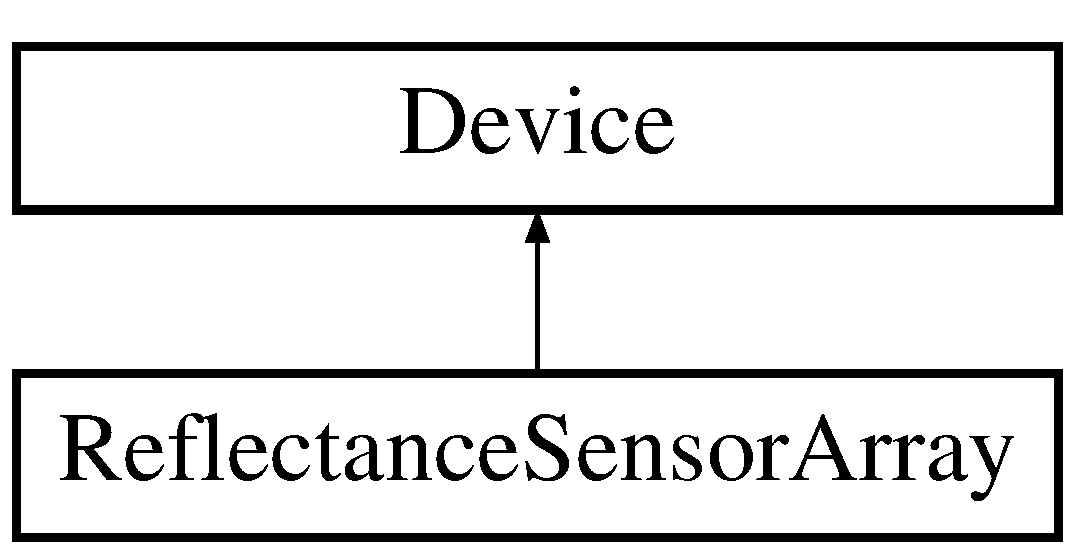
\includegraphics[height=2.000000cm]{classReflectanceSensorArray}
\end{center}
\end{figure}
\subsection*{Métodos Públicos}
\begin{DoxyCompactItemize}
\item 
\hyperlink{classReflectanceSensorArray_a4e1aebfbf34f73ac86628213dfa106e7}{Reflectance\-Sensor\-Array} (uint8\-\_\-t pin\-\_\-out, const uint8\-\_\-t pins\-\_\-sel\mbox{[}$\,$\mbox{]}, uint16\-\_\-t thld)
\item 
\hyperlink{classReflectanceSensorArray_a8597647e8737a1a868dc8240e12774f1}{Reflectance\-Sensor\-Array} (const uint8\-\_\-t pins\mbox{[}$\,$\mbox{]})
\item 
void \hyperlink{classReflectanceSensorArray_a11602e4c9b93577608b07088f9c0fd3c}{begin} ()
\begin{DoxyCompactList}\small\item\em Inicializa o dispositivo. \end{DoxyCompactList}\item 
void \hyperlink{classReflectanceSensorArray_ae83ddbd02df0b879bf67c99a02341f2b}{stop} ()
\begin{DoxyCompactList}\small\item\em Interrompe o funcionamento do dispositivo. \end{DoxyCompactList}\item 
void \hyperlink{classReflectanceSensorArray_aed9eaebad7add3ac016ea8af942261a5}{reset} ()
\begin{DoxyCompactList}\small\item\em Redefine o estado do dispositivo. \end{DoxyCompactList}\item 
void \hyperlink{classReflectanceSensorArray_a3a5f7c29c3a72026365df9cf9791e3e5}{update} ()
\begin{DoxyCompactList}\small\item\em Atualiza o estado atual do dispositivo. \end{DoxyCompactList}\item 
bool \hyperlink{classReflectanceSensorArray_a7781688e68d77cce4f7c70bbe242113b}{is\-Ready} ()
\begin{DoxyCompactList}\small\item\em Verifica se o dispositivo está pronto para receber novos comandos ou leituras. \end{DoxyCompactList}\item 
uint8\-\_\-t \hyperlink{classReflectanceSensorArray_ad608c5f45ea98fe65162d8c24722bc15}{get} (uint8\-\_\-t $\ast$buffer, uint8\-\_\-t size)
\item 
void \hyperlink{classReflectanceSensorArray_a023408b8b40cea4a74c5c1837a39d701}{set} (const uint8\-\_\-t $\ast$data, uint8\-\_\-t size=1)
\end{DoxyCompactItemize}


\subsection{Construtores \& Destrutores}
\hypertarget{classReflectanceSensorArray_a4e1aebfbf34f73ac86628213dfa106e7}{\index{Reflectance\-Sensor\-Array@{Reflectance\-Sensor\-Array}!Reflectance\-Sensor\-Array@{Reflectance\-Sensor\-Array}}
\index{Reflectance\-Sensor\-Array@{Reflectance\-Sensor\-Array}!ReflectanceSensorArray@{Reflectance\-Sensor\-Array}}
\subsubsection[{Reflectance\-Sensor\-Array}]{\setlength{\rightskip}{0pt plus 5cm}Reflectance\-Sensor\-Array\-::\-Reflectance\-Sensor\-Array (
\begin{DoxyParamCaption}
\item[{uint8\-\_\-t}]{pin\-\_\-out, }
\item[{const uint8\-\_\-t}]{pins\-\_\-sel\mbox{[}$\,$\mbox{]}, }
\item[{uint16\-\_\-t}]{thld}
\end{DoxyParamCaption}
)}}\label{classReflectanceSensorArray_a4e1aebfbf34f73ac86628213dfa106e7}
\hypertarget{classReflectanceSensorArray_a8597647e8737a1a868dc8240e12774f1}{\index{Reflectance\-Sensor\-Array@{Reflectance\-Sensor\-Array}!Reflectance\-Sensor\-Array@{Reflectance\-Sensor\-Array}}
\index{Reflectance\-Sensor\-Array@{Reflectance\-Sensor\-Array}!ReflectanceSensorArray@{Reflectance\-Sensor\-Array}}
\subsubsection[{Reflectance\-Sensor\-Array}]{\setlength{\rightskip}{0pt plus 5cm}Reflectance\-Sensor\-Array\-::\-Reflectance\-Sensor\-Array (
\begin{DoxyParamCaption}
\item[{const uint8\-\_\-t}]{pins\mbox{[}$\,$\mbox{]}}
\end{DoxyParamCaption}
)}}\label{classReflectanceSensorArray_a8597647e8737a1a868dc8240e12774f1}


\subsection{Métodos}
\hypertarget{classReflectanceSensorArray_a11602e4c9b93577608b07088f9c0fd3c}{\index{Reflectance\-Sensor\-Array@{Reflectance\-Sensor\-Array}!begin@{begin}}
\index{begin@{begin}!ReflectanceSensorArray@{Reflectance\-Sensor\-Array}}
\subsubsection[{begin}]{\setlength{\rightskip}{0pt plus 5cm}void Reflectance\-Sensor\-Array\-::begin (
\begin{DoxyParamCaption}
{}
\end{DoxyParamCaption}
)\hspace{0.3cm}{\ttfamily [virtual]}}}\label{classReflectanceSensorArray_a11602e4c9b93577608b07088f9c0fd3c}


Inicializa o dispositivo. 

Esta função é executada apenas uma vez em \hyperlink{classRobot_a6c7ee2437ae5427a19f2de4903ca0df9}{Robot\-::begin()}. 

Implementa \hyperlink{classDevice_a0dc99b16a220489d787a1cbcef4875d9}{Device}.

\hypertarget{classReflectanceSensorArray_ad608c5f45ea98fe65162d8c24722bc15}{\index{Reflectance\-Sensor\-Array@{Reflectance\-Sensor\-Array}!get@{get}}
\index{get@{get}!ReflectanceSensorArray@{Reflectance\-Sensor\-Array}}
\subsubsection[{get}]{\setlength{\rightskip}{0pt plus 5cm}uint8\-\_\-t Reflectance\-Sensor\-Array\-::get (
\begin{DoxyParamCaption}
\item[{uint8\-\_\-t $\ast$}]{buffer, }
\item[{uint8\-\_\-t}]{size}
\end{DoxyParamCaption}
)\hspace{0.3cm}{\ttfamily [virtual]}}}\label{classReflectanceSensorArray_ad608c5f45ea98fe65162d8c24722bc15}

\begin{DoxyParams}[1]{Parâmetros}
\mbox{\tt out}  & {\em buffer} & Array de bytes com tamanho suficiente para armazenar a resposta. \\
\hline
 & {\em size} & Tamanho do {\ttfamily buffer}.\\
\hline
\end{DoxyParams}
\begin{DoxyReturn}{Retorna}
O numero de bytes escritos em {\ttfamily buffer}. 
\end{DoxyReturn}


Implementa \hyperlink{classDevice_a0057af09515609c289d5da3be19dcc8d}{Device}.

\hypertarget{classReflectanceSensorArray_a7781688e68d77cce4f7c70bbe242113b}{\index{Reflectance\-Sensor\-Array@{Reflectance\-Sensor\-Array}!is\-Ready@{is\-Ready}}
\index{is\-Ready@{is\-Ready}!ReflectanceSensorArray@{Reflectance\-Sensor\-Array}}
\subsubsection[{is\-Ready}]{\setlength{\rightskip}{0pt plus 5cm}bool Reflectance\-Sensor\-Array\-::is\-Ready (
\begin{DoxyParamCaption}
{}
\end{DoxyParamCaption}
)\hspace{0.3cm}{\ttfamily [virtual]}}}\label{classReflectanceSensorArray_a7781688e68d77cce4f7c70bbe242113b}


Verifica se o dispositivo está pronto para receber novos comandos ou leituras. 

É importante para \hyperlink{classRobot}{Robot} definir se uma ação de maior grau de abstração foi concluída ou não.

\begin{DoxyReturn}{Retorna}
{\ttfamily T\-R\-U\-E} se o dispositivo está ocioso. 
\end{DoxyReturn}


Implementa \hyperlink{classDevice_a30065df084d450dbaae9d68215e01e6f}{Device}.

\hypertarget{classReflectanceSensorArray_aed9eaebad7add3ac016ea8af942261a5}{\index{Reflectance\-Sensor\-Array@{Reflectance\-Sensor\-Array}!reset@{reset}}
\index{reset@{reset}!ReflectanceSensorArray@{Reflectance\-Sensor\-Array}}
\subsubsection[{reset}]{\setlength{\rightskip}{0pt plus 5cm}void Reflectance\-Sensor\-Array\-::reset (
\begin{DoxyParamCaption}
{}
\end{DoxyParamCaption}
)\hspace{0.3cm}{\ttfamily [virtual]}}}\label{classReflectanceSensorArray_aed9eaebad7add3ac016ea8af942261a5}


Redefine o estado do dispositivo. 



Implementa \hyperlink{classDevice_a6e43162e890cb40eafb923b0c94d167a}{Device}.

\hypertarget{classReflectanceSensorArray_a023408b8b40cea4a74c5c1837a39d701}{\index{Reflectance\-Sensor\-Array@{Reflectance\-Sensor\-Array}!set@{set}}
\index{set@{set}!ReflectanceSensorArray@{Reflectance\-Sensor\-Array}}
\subsubsection[{set}]{\setlength{\rightskip}{0pt plus 5cm}void Reflectance\-Sensor\-Array\-::set (
\begin{DoxyParamCaption}
\item[{const uint8\-\_\-t $\ast$}]{data, }
\item[{uint8\-\_\-t}]{size = {\ttfamily 1}}
\end{DoxyParamCaption}
)\hspace{0.3cm}{\ttfamily [virtual]}}}\label{classReflectanceSensorArray_a023408b8b40cea4a74c5c1837a39d701}

\begin{DoxyParams}[1]{Parâmetros}
\mbox{\tt in}  & {\em data} & Mensagem a ser processada pelo dispositivo. \\
\hline
 & {\em size} & Tamanho do vetor data. \\
\hline
\end{DoxyParams}


Implementa \hyperlink{classDevice_a3b4bf3ff761f93c024675548755586d8}{Device}.

\hypertarget{classReflectanceSensorArray_ae83ddbd02df0b879bf67c99a02341f2b}{\index{Reflectance\-Sensor\-Array@{Reflectance\-Sensor\-Array}!stop@{stop}}
\index{stop@{stop}!ReflectanceSensorArray@{Reflectance\-Sensor\-Array}}
\subsubsection[{stop}]{\setlength{\rightskip}{0pt plus 5cm}void Reflectance\-Sensor\-Array\-::stop (
\begin{DoxyParamCaption}
{}
\end{DoxyParamCaption}
)\hspace{0.3cm}{\ttfamily [virtual]}}}\label{classReflectanceSensorArray_ae83ddbd02df0b879bf67c99a02341f2b}


Interrompe o funcionamento do dispositivo. 



Implementa \hyperlink{classDevice_a22430f274658b04c280b5cc2d53aa1e4}{Device}.

\hypertarget{classReflectanceSensorArray_a3a5f7c29c3a72026365df9cf9791e3e5}{\index{Reflectance\-Sensor\-Array@{Reflectance\-Sensor\-Array}!update@{update}}
\index{update@{update}!ReflectanceSensorArray@{Reflectance\-Sensor\-Array}}
\subsubsection[{update}]{\setlength{\rightskip}{0pt plus 5cm}void Reflectance\-Sensor\-Array\-::update (
\begin{DoxyParamCaption}
{}
\end{DoxyParamCaption}
)\hspace{0.3cm}{\ttfamily [virtual]}}}\label{classReflectanceSensorArray_a3a5f7c29c3a72026365df9cf9791e3e5}


Atualiza o estado atual do dispositivo. 

Esta função é executada uma vez a cada \hyperlink{classRobot_aa50d73cd1109a70133af442674ed3a1a}{Robot\-::step()}. 

Implementa \hyperlink{classDevice_a7e5226b6341b1cf2ec04a5913b97becc}{Device}.



A documentação para esta classe foi gerada a partir dos seguintes arquivos\-:\begin{DoxyCompactItemize}
\item 
\hyperlink{ReflectanceSensorArray_8h}{Reflectance\-Sensor\-Array.\-h}\item 
\hyperlink{ReflectanceSensorArray_8cpp}{Reflectance\-Sensor\-Array.\-cpp}\end{DoxyCompactItemize}

\hypertarget{classRobot}{\section{Referência da Classe Robot}
\label{classRobot}\index{Robot@{Robot}}
}


A classe \hyperlink{classRobot}{Robot} representa um robô simples, seja ele autonomo ou não, o mesmo possui dispositivos (\hyperlink{classDevice}{Device}), que obtem valores do ambiente e realizam ações físicas, e conexões (\hyperlink{classConnection}{Connection}) as quais permitem que ele se comunique com computadores, microcontroladores ou outros robôs.  




{\ttfamily \#include $<$Robot.\-h$>$}

Diagrama de Hierarquia para Robot\-:\begin{figure}[H]
\begin{center}
\leavevmode
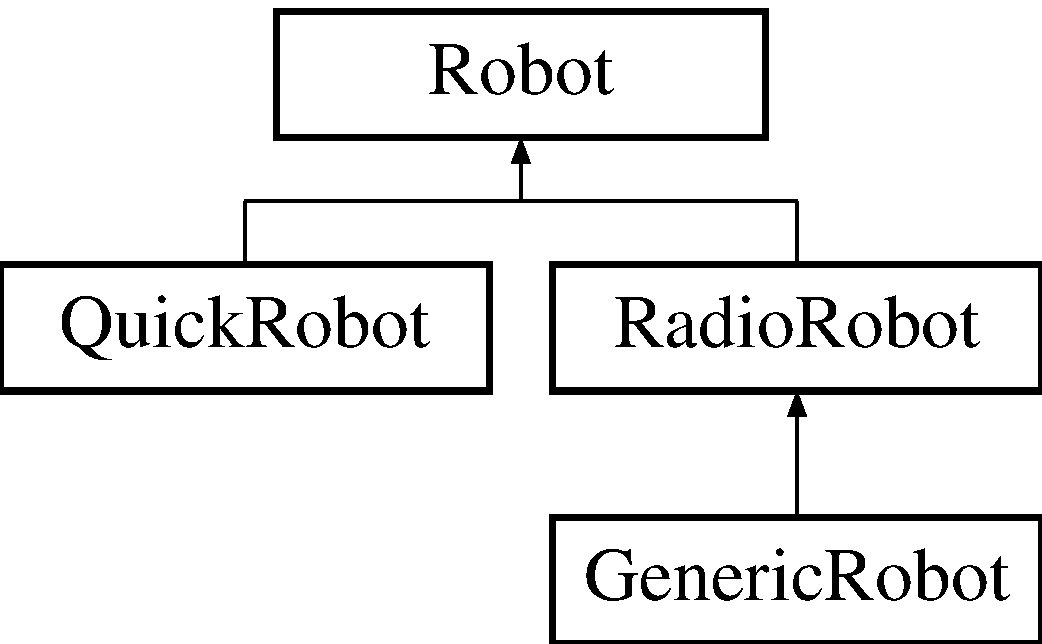
\includegraphics[height=3.000000cm]{classRobot}
\end{center}
\end{figure}
\subsection*{Métodos Públicos}
\begin{DoxyCompactItemize}
\item 
\hyperlink{classRobot_a4fc7c70ae20623f05e06f2ecb388b6c4}{Robot} ()
\begin{DoxyCompactList}\small\item\em Construtor padrão. \end{DoxyCompactList}\item 
void \hyperlink{classRobot_a6c7ee2437ae5427a19f2de4903ca0df9}{begin} ()
\begin{DoxyCompactList}\small\item\em Inicializa o robô. \end{DoxyCompactList}\item 
void \hyperlink{classRobot_af59eb38f118092bd3369876a2aaac2d1}{add\-Connection} (\hyperlink{classConnection}{Connection} \&c)
\begin{DoxyCompactList}\small\item\em Adiciona uma nova conexão. \end{DoxyCompactList}\item 
void \hyperlink{classRobot_a3a965a448c5d9d95ecb2bf6c5ee668b9}{add\-Device} (\hyperlink{classDevice}{Device} \&d)
\begin{DoxyCompactList}\small\item\em Adiciona um novo dispositivo. \end{DoxyCompactList}\item 
bool \hyperlink{classRobot_a1c344a898d9da75010438fd78d3827b2}{is\-Busy} ()
\begin{DoxyCompactList}\small\item\em Verifica se existe algum dispositivo ocupado. \end{DoxyCompactList}\item 
void \hyperlink{classRobot_aa50d73cd1109a70133af442674ed3a1a}{step} ()
\begin{DoxyCompactList}\small\item\em Realiza o escalonamento de todas as funções principais do robô. \end{DoxyCompactList}\item 
void \hyperlink{classRobot_aaad55dfa6b3daedd9670bec46dc079f1}{perform} ()
\begin{DoxyCompactList}\small\item\em Realiza todas as ações pendentes e retorna. \end{DoxyCompactList}\item 
\hyperlink{classClock}{Clock} \& \hyperlink{classRobot_af96d177958b4b3087aba65d1cc4c06b6}{get\-Clock} ()
\begin{DoxyCompactList}\small\item\em T\-O\-D\-O. \end{DoxyCompactList}\item 
virtual void \hyperlink{classRobot_ab02c09bdea244d38bcfd0010b9554b6f}{message\-Received} (const uint8\-\_\-t $\ast$data, uint8\-\_\-t size, \hyperlink{classConnection}{Connection} \&connection)=0
\begin{DoxyCompactList}\small\item\em Função executada quando uma mensagem é recebida por alguma conexão. \end{DoxyCompactList}\item 
virtual void \hyperlink{classRobot_aaa0c932d862aed7556b068ebb70a917a}{device\-Ready} (\hyperlink{classDevice}{Device} \&d)=0
\begin{DoxyCompactList}\small\item\em Função executada quando um dispositivo anteriormente ocupado torna-\/se disponível. \end{DoxyCompactList}\item 
virtual void \hyperlink{classRobot_a75cfdd8e35e007abe24ffae66a8ecf1d}{think} ()=0
\begin{DoxyCompactList}\small\item\em Função responsável por tomar novas decisões com base nos sensores e atuadores do robô, em um determinado ciclo. \end{DoxyCompactList}\end{DoxyCompactItemize}
\subsection*{Métodos Protegidos}
\begin{DoxyCompactItemize}
\item 
uint8\-\_\-t \hyperlink{classRobot_a6ef66669b08d6c17e249d946eec87f2d}{get\-Connection\-List\-Size} ()
\begin{DoxyCompactList}\small\item\em Obtem o tamanho da lista de conexões disponiveis. \end{DoxyCompactList}\item 
uint8\-\_\-t \hyperlink{classRobot_a09b95280d83027439d27749ba2c0bc4a}{get\-Device\-List\-Size} ()
\begin{DoxyCompactList}\small\item\em Obtem o tamanho da lista de dispositivos disponiveis. \end{DoxyCompactList}\item 
\hyperlink{classConnection}{Connection} $\ast$ \hyperlink{classRobot_a6e96ee4f33816dd91cd76d950e134b53}{get\-Connection} (uint8\-\_\-t index)
\begin{DoxyCompactList}\small\item\em Obtem uma determinada conexão. \end{DoxyCompactList}\item 
\hyperlink{classDevice}{Device} $\ast$ \hyperlink{classRobot_af5e50d99c051a6b25dfc561535111444}{get\-Device} (uint8\-\_\-t index)
\begin{DoxyCompactList}\small\item\em Obtem um determinado dispositivo. \end{DoxyCompactList}\end{DoxyCompactItemize}
\subsection*{Atributos Protegidos}
\begin{DoxyCompactItemize}
\item 
uint8\-\_\-t $\ast$ \hyperlink{classRobot_aef6f636eb10e6b4998a3b1859ca71500}{buffer}
\begin{DoxyCompactList}\small\item\em Buffer para o recebimento das mensagens, o mesmo é encaminhado para {\ttfamily message\-Received}. \end{DoxyCompactList}\end{DoxyCompactItemize}
\subsection*{Atributos Estáticos Protegidos}
\begin{DoxyCompactItemize}
\item 
static \hyperlink{classClock}{Clock} \& \hyperlink{classRobot_a9bc655119fd6d2864c6aca60403c282d}{clock} = \hyperlink{Robot_8cpp_aa917eb258987bd1c3d34d4972b7cc783}{\-\_\-g\-Clock}
\end{DoxyCompactItemize}
\subsection*{Amigas}
\begin{DoxyCompactItemize}
\item 
class \hyperlink{classRobot_a59d051cd870745df59aefaa2cda15b8a}{Timed\-Device}
\end{DoxyCompactItemize}


\subsection{Descrição Detalhada}
A classe \hyperlink{classRobot}{Robot} representa um robô simples, seja ele autonomo ou não, o mesmo possui dispositivos (\hyperlink{classDevice}{Device}), que obtem valores do ambiente e realizam ações físicas, e conexões (\hyperlink{classConnection}{Connection}) as quais permitem que ele se comunique com computadores, microcontroladores ou outros robôs. 

\subsection{Construtores \& Destrutores}
\hypertarget{classRobot_a4fc7c70ae20623f05e06f2ecb388b6c4}{\index{Robot@{Robot}!Robot@{Robot}}
\index{Robot@{Robot}!Robot@{Robot}}
\subsubsection[{Robot}]{\setlength{\rightskip}{0pt plus 5cm}Robot\-::\-Robot (
\begin{DoxyParamCaption}
{}
\end{DoxyParamCaption}
)\hspace{0.3cm}{\ttfamily [inline]}}}\label{classRobot_a4fc7c70ae20623f05e06f2ecb388b6c4}


Construtor padrão. 



\subsection{Métodos}
\hypertarget{classRobot_af59eb38f118092bd3369876a2aaac2d1}{\index{Robot@{Robot}!add\-Connection@{add\-Connection}}
\index{add\-Connection@{add\-Connection}!Robot@{Robot}}
\subsubsection[{add\-Connection}]{\setlength{\rightskip}{0pt plus 5cm}void Robot\-::add\-Connection (
\begin{DoxyParamCaption}
\item[{{\bf Connection} \&}]{c}
\end{DoxyParamCaption}
)}}\label{classRobot_af59eb38f118092bd3369876a2aaac2d1}


Adiciona uma nova conexão. 


\begin{DoxyParams}{Parâmetros}
{\em c} & Referência da conexão. \\
\hline
\end{DoxyParams}
\hypertarget{classRobot_a3a965a448c5d9d95ecb2bf6c5ee668b9}{\index{Robot@{Robot}!add\-Device@{add\-Device}}
\index{add\-Device@{add\-Device}!Robot@{Robot}}
\subsubsection[{add\-Device}]{\setlength{\rightskip}{0pt plus 5cm}void Robot\-::add\-Device (
\begin{DoxyParamCaption}
\item[{{\bf Device} \&}]{d}
\end{DoxyParamCaption}
)}}\label{classRobot_a3a965a448c5d9d95ecb2bf6c5ee668b9}


Adiciona um novo dispositivo. 


\begin{DoxyParams}{Parâmetros}
{\em d} & Referência do dispositivo. \\
\hline
\end{DoxyParams}
\hypertarget{classRobot_a6c7ee2437ae5427a19f2de4903ca0df9}{\index{Robot@{Robot}!begin@{begin}}
\index{begin@{begin}!Robot@{Robot}}
\subsubsection[{begin}]{\setlength{\rightskip}{0pt plus 5cm}void Robot\-::begin (
\begin{DoxyParamCaption}
{}
\end{DoxyParamCaption}
)}}\label{classRobot_a6c7ee2437ae5427a19f2de4903ca0df9}


Inicializa o robô. 

Deve ser chamado em {\ttfamily Setup()} apenas uma vez. É responsável por inicializar todas as conexões e dispositivos integrados ao robô. \hypertarget{classRobot_aaa0c932d862aed7556b068ebb70a917a}{\index{Robot@{Robot}!device\-Ready@{device\-Ready}}
\index{device\-Ready@{device\-Ready}!Robot@{Robot}}
\subsubsection[{device\-Ready}]{\setlength{\rightskip}{0pt plus 5cm}virtual void Robot\-::device\-Ready (
\begin{DoxyParamCaption}
\item[{{\bf Device} \&}]{d}
\end{DoxyParamCaption}
)\hspace{0.3cm}{\ttfamily [pure virtual]}}}\label{classRobot_aaa0c932d862aed7556b068ebb70a917a}


Função executada quando um dispositivo anteriormente ocupado torna-\/se disponível. 


\begin{DoxyParams}{Parâmetros}
{\em d} & Referência ao dispositivo em questão. \\
\hline
\end{DoxyParams}


Implementado por \hyperlink{classQuickRobot_a95d490eb2e580d362b99eb6c90927256}{Quick\-Robot} e \hyperlink{classRadioRobot_a278b37c78b4fd9c4d7b16192e780f6a1}{Radio\-Robot}.

\hypertarget{classRobot_af96d177958b4b3087aba65d1cc4c06b6}{\index{Robot@{Robot}!get\-Clock@{get\-Clock}}
\index{get\-Clock@{get\-Clock}!Robot@{Robot}}
\subsubsection[{get\-Clock}]{\setlength{\rightskip}{0pt plus 5cm}{\bf Clock}\& Robot\-::get\-Clock (
\begin{DoxyParamCaption}
{}
\end{DoxyParamCaption}
)\hspace{0.3cm}{\ttfamily [inline]}}}\label{classRobot_af96d177958b4b3087aba65d1cc4c06b6}


T\-O\-D\-O. 

\hypertarget{classRobot_a6e96ee4f33816dd91cd76d950e134b53}{\index{Robot@{Robot}!get\-Connection@{get\-Connection}}
\index{get\-Connection@{get\-Connection}!Robot@{Robot}}
\subsubsection[{get\-Connection}]{\setlength{\rightskip}{0pt plus 5cm}{\bf Connection} $\ast$ Robot\-::get\-Connection (
\begin{DoxyParamCaption}
\item[{uint8\-\_\-t}]{index}
\end{DoxyParamCaption}
)\hspace{0.3cm}{\ttfamily [protected]}}}\label{classRobot_a6e96ee4f33816dd91cd76d950e134b53}


Obtem uma determinada conexão. 


\begin{DoxyParams}{Parâmetros}
{\em index} & Indice do dispositivo. \\
\hline
\end{DoxyParams}
\begin{DoxyReturn}{Retorna}
Um ponteiro para a conexão ou {\ttfamily N\-U\-L\-L} 
\end{DoxyReturn}
\hypertarget{classRobot_a6ef66669b08d6c17e249d946eec87f2d}{\index{Robot@{Robot}!get\-Connection\-List\-Size@{get\-Connection\-List\-Size}}
\index{get\-Connection\-List\-Size@{get\-Connection\-List\-Size}!Robot@{Robot}}
\subsubsection[{get\-Connection\-List\-Size}]{\setlength{\rightskip}{0pt plus 5cm}uint8\-\_\-t Robot\-::get\-Connection\-List\-Size (
\begin{DoxyParamCaption}
{}
\end{DoxyParamCaption}
)\hspace{0.3cm}{\ttfamily [protected]}}}\label{classRobot_a6ef66669b08d6c17e249d946eec87f2d}


Obtem o tamanho da lista de conexões disponiveis. 

\begin{DoxyReturn}{Retorna}
O tamanho da lista {\ttfamily }(n$>$=0) 
\end{DoxyReturn}
\hypertarget{classRobot_af5e50d99c051a6b25dfc561535111444}{\index{Robot@{Robot}!get\-Device@{get\-Device}}
\index{get\-Device@{get\-Device}!Robot@{Robot}}
\subsubsection[{get\-Device}]{\setlength{\rightskip}{0pt plus 5cm}{\bf Device} $\ast$ Robot\-::get\-Device (
\begin{DoxyParamCaption}
\item[{uint8\-\_\-t}]{index}
\end{DoxyParamCaption}
)\hspace{0.3cm}{\ttfamily [protected]}}}\label{classRobot_af5e50d99c051a6b25dfc561535111444}


Obtem um determinado dispositivo. 


\begin{DoxyParams}{Parâmetros}
{\em index} & Indice do dispositivo. \\
\hline
\end{DoxyParams}
\begin{DoxyReturn}{Retorna}
Um ponteiro para o dispositivo ou {\ttfamily N\-U\-L\-L} 
\end{DoxyReturn}
\hypertarget{classRobot_a09b95280d83027439d27749ba2c0bc4a}{\index{Robot@{Robot}!get\-Device\-List\-Size@{get\-Device\-List\-Size}}
\index{get\-Device\-List\-Size@{get\-Device\-List\-Size}!Robot@{Robot}}
\subsubsection[{get\-Device\-List\-Size}]{\setlength{\rightskip}{0pt plus 5cm}uint8\-\_\-t Robot\-::get\-Device\-List\-Size (
\begin{DoxyParamCaption}
{}
\end{DoxyParamCaption}
)\hspace{0.3cm}{\ttfamily [protected]}}}\label{classRobot_a09b95280d83027439d27749ba2c0bc4a}


Obtem o tamanho da lista de dispositivos disponiveis. 

\begin{DoxyReturn}{Retorna}
O tamanho da lista {\ttfamily }(n$>$=0) 
\end{DoxyReturn}
\hypertarget{classRobot_a1c344a898d9da75010438fd78d3827b2}{\index{Robot@{Robot}!is\-Busy@{is\-Busy}}
\index{is\-Busy@{is\-Busy}!Robot@{Robot}}
\subsubsection[{is\-Busy}]{\setlength{\rightskip}{0pt plus 5cm}bool Robot\-::is\-Busy (
\begin{DoxyParamCaption}
{}
\end{DoxyParamCaption}
)}}\label{classRobot_a1c344a898d9da75010438fd78d3827b2}


Verifica se existe algum dispositivo ocupado. 

\begin{DoxyReturn}{Retorna}
{\ttfamily true} se existe algum dispositivo ocupado. 
\end{DoxyReturn}
\hypertarget{classRobot_ab02c09bdea244d38bcfd0010b9554b6f}{\index{Robot@{Robot}!message\-Received@{message\-Received}}
\index{message\-Received@{message\-Received}!Robot@{Robot}}
\subsubsection[{message\-Received}]{\setlength{\rightskip}{0pt plus 5cm}virtual void Robot\-::message\-Received (
\begin{DoxyParamCaption}
\item[{const uint8\-\_\-t $\ast$}]{data, }
\item[{uint8\-\_\-t}]{size, }
\item[{{\bf Connection} \&}]{connection}
\end{DoxyParamCaption}
)\hspace{0.3cm}{\ttfamily [pure virtual]}}}\label{classRobot_ab02c09bdea244d38bcfd0010b9554b6f}


Função executada quando uma mensagem é recebida por alguma conexão. 


\begin{DoxyParams}[1]{Parâmetros}
\mbox{\tt in}  & {\em data} & Um vetor de constantes de 8bits (byte) contendo a mensagem. \\
\hline
 & {\em size} & O tamanho da mensagem em bytes. \\
\hline
 & {\em connection} & O I\-D da conexão que recebeu a mensagem. \\
\hline
\end{DoxyParams}


Implementado por \hyperlink{classQuickRobot_a96eda0e5288726364f4a02ef7912e21b}{Quick\-Robot} e \hyperlink{classRadioRobot_a5de90c99faa941df35898349b6b148b5}{Radio\-Robot}.

\hypertarget{classRobot_aaad55dfa6b3daedd9670bec46dc079f1}{\index{Robot@{Robot}!perform@{perform}}
\index{perform@{perform}!Robot@{Robot}}
\subsubsection[{perform}]{\setlength{\rightskip}{0pt plus 5cm}void Robot\-::perform (
\begin{DoxyParamCaption}
{}
\end{DoxyParamCaption}
)}}\label{classRobot_aaad55dfa6b3daedd9670bec46dc079f1}


Realiza todas as ações pendentes e retorna. 

Útil para programar as ações do robô em uma sequência. \hypertarget{classRobot_aa50d73cd1109a70133af442674ed3a1a}{\index{Robot@{Robot}!step@{step}}
\index{step@{step}!Robot@{Robot}}
\subsubsection[{step}]{\setlength{\rightskip}{0pt plus 5cm}void Robot\-::step (
\begin{DoxyParamCaption}
{}
\end{DoxyParamCaption}
)}}\label{classRobot_aa50d73cd1109a70133af442674ed3a1a}


Realiza o escalonamento de todas as funções principais do robô. 

É nessa função que sao executadas \hyperlink{classDevice_a7e5226b6341b1cf2ec04a5913b97becc}{Device\-::update()}, e \hyperlink{classRobot_a75cfdd8e35e007abe24ffae66a8ecf1d}{Robot\-::think()} e é verificado por novas mensagens por meio de \hyperlink{classConnection_acd5ee426481b2aca2903d96f6f807341}{Connection\-::available()}. \hypertarget{classRobot_a75cfdd8e35e007abe24ffae66a8ecf1d}{\index{Robot@{Robot}!think@{think}}
\index{think@{think}!Robot@{Robot}}
\subsubsection[{think}]{\setlength{\rightskip}{0pt plus 5cm}virtual void Robot\-::think (
\begin{DoxyParamCaption}
{}
\end{DoxyParamCaption}
)\hspace{0.3cm}{\ttfamily [pure virtual]}}}\label{classRobot_a75cfdd8e35e007abe24ffae66a8ecf1d}


Função responsável por tomar novas decisões com base nos sensores e atuadores do robô, em um determinado ciclo. 

É executada uma vez a cada \hyperlink{classRobot_aa50d73cd1109a70133af442674ed3a1a}{Robot\-::step()}. 

Implementado por \hyperlink{classQuickRobot_a936a04970e2fe8694256a70816b697f6}{Quick\-Robot} e \hyperlink{classRadioRobot_a7b58f55a81e816ba5d53fd14bf28a6a5}{Radio\-Robot}.



\subsection{Amigas e Funções Relacionadas}
\hypertarget{classRobot_a59d051cd870745df59aefaa2cda15b8a}{\index{Robot@{Robot}!Timed\-Device@{Timed\-Device}}
\index{Timed\-Device@{Timed\-Device}!Robot@{Robot}}
\subsubsection[{Timed\-Device}]{\setlength{\rightskip}{0pt plus 5cm}friend class {\bf Timed\-Device}\hspace{0.3cm}{\ttfamily [friend]}}}\label{classRobot_a59d051cd870745df59aefaa2cda15b8a}


\subsection{Atributos}
\hypertarget{classRobot_aef6f636eb10e6b4998a3b1859ca71500}{\index{Robot@{Robot}!buffer@{buffer}}
\index{buffer@{buffer}!Robot@{Robot}}
\subsubsection[{buffer}]{\setlength{\rightskip}{0pt plus 5cm}uint8\-\_\-t$\ast$ Robot\-::buffer\hspace{0.3cm}{\ttfamily [protected]}}}\label{classRobot_aef6f636eb10e6b4998a3b1859ca71500}


Buffer para o recebimento das mensagens, o mesmo é encaminhado para {\ttfamily message\-Received}. 

\hypertarget{classRobot_a9bc655119fd6d2864c6aca60403c282d}{\index{Robot@{Robot}!clock@{clock}}
\index{clock@{clock}!Robot@{Robot}}
\subsubsection[{clock}]{\setlength{\rightskip}{0pt plus 5cm}{\bf Clock} \& Robot\-::clock = {\bf \-\_\-g\-Clock}\hspace{0.3cm}{\ttfamily [static]}, {\ttfamily [protected]}}}\label{classRobot_a9bc655119fd6d2864c6aca60403c282d}


A documentação para esta classe foi gerada a partir dos seguintes arquivos\-:\begin{DoxyCompactItemize}
\item 
\hyperlink{Robot_8h}{Robot.\-h}\item 
\hyperlink{Robot_8cpp}{Robot.\-cpp}\end{DoxyCompactItemize}

\hypertarget{classSerialConnection}{\section{Referência da Classe Serial\-Connection}
\label{classSerialConnection}\index{Serial\-Connection@{Serial\-Connection}}
}


{\ttfamily \#include $<$Serial\-Connection.\-h$>$}

Diagrama de Hierarquia para Serial\-Connection\-:\begin{figure}[H]
\begin{center}
\leavevmode
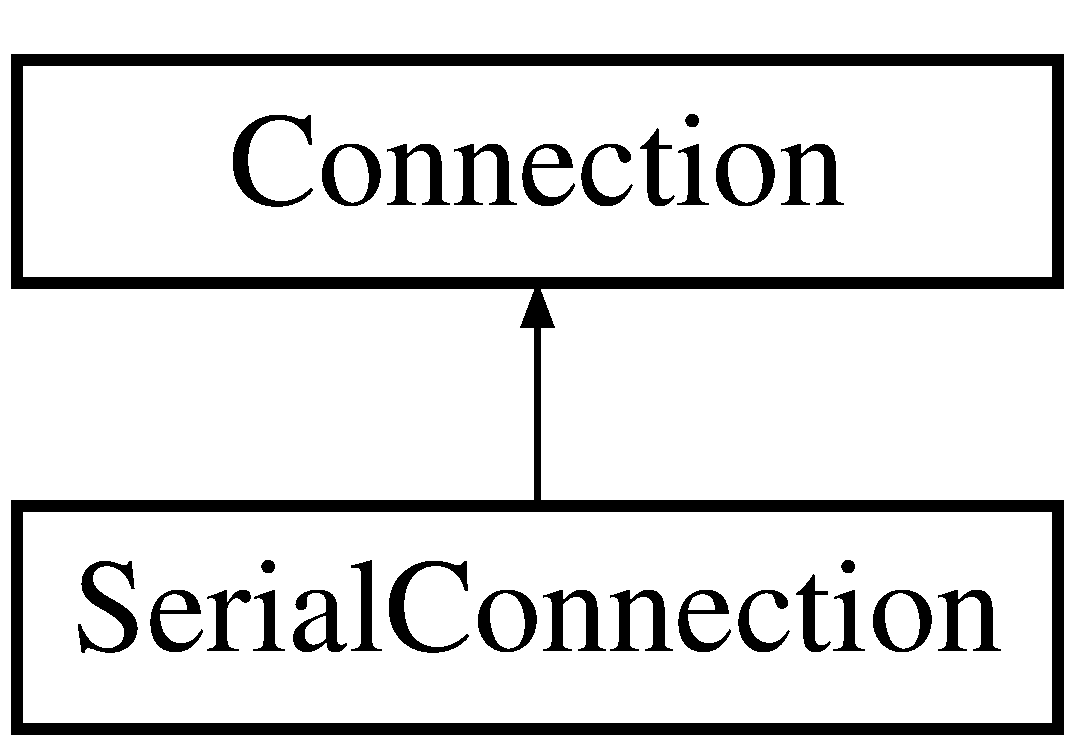
\includegraphics[height=2.000000cm]{classSerialConnection}
\end{center}
\end{figure}
\subsection*{Métodos Públicos}
\begin{DoxyCompactItemize}
\item 
\hyperlink{classSerialConnection_a05e15045efc5ea7098337f9dcd43fc82}{Serial\-Connection} (Hardware\-Serial \&the\-Serial, uint32\-\_\-t rate)
\item 
void \hyperlink{classSerialConnection_a6022b91cdd0bc412d8aeda364c32ce21}{begin} ()
\begin{DoxyCompactList}\small\item\em Inicializa a conexão. \end{DoxyCompactList}\item 
uint8\-\_\-t \hyperlink{classSerialConnection_a91aa59d8f0b913e91dc4ddcde8e42519}{available} ()
\begin{DoxyCompactList}\small\item\em Verifica se existe alguma mensagem disponivel. \end{DoxyCompactList}\item 
void \hyperlink{classSerialConnection_a85e05ec34dbb4d8d6feaccecf8ae9a72}{println} (const char $\ast$data)
\item 
bool \hyperlink{classSerialConnection_ac98733956090bc3eaa628d156f06ef5d}{send\-Message} (const uint8\-\_\-t $\ast$data, uint8\-\_\-t size)
\begin{DoxyCompactList}\small\item\em Envia uma mensagem. \end{DoxyCompactList}\item 
uint8\-\_\-t \hyperlink{classSerialConnection_ac72ec887122fe08fd389dc8724b31c63}{receive\-Message} (uint8\-\_\-t $\ast$buffer, uint8\-\_\-t size)
\begin{DoxyCompactList}\small\item\em Recebe uma mensagem. \end{DoxyCompactList}\item 
Hardware\-Serial \& \hyperlink{classSerialConnection_af5aff354718e4912d80fcee953d54540}{get\-Port} ()
\end{DoxyCompactItemize}


\subsection{Construtores \& Destrutores}
\hypertarget{classSerialConnection_a05e15045efc5ea7098337f9dcd43fc82}{\index{Serial\-Connection@{Serial\-Connection}!Serial\-Connection@{Serial\-Connection}}
\index{Serial\-Connection@{Serial\-Connection}!SerialConnection@{Serial\-Connection}}
\subsubsection[{Serial\-Connection}]{\setlength{\rightskip}{0pt plus 5cm}Serial\-Connection\-::\-Serial\-Connection (
\begin{DoxyParamCaption}
\item[{Hardware\-Serial \&}]{the\-Serial, }
\item[{uint32\-\_\-t}]{rate}
\end{DoxyParamCaption}
)}}\label{classSerialConnection_a05e15045efc5ea7098337f9dcd43fc82}


\subsection{Métodos}
\hypertarget{classSerialConnection_a91aa59d8f0b913e91dc4ddcde8e42519}{\index{Serial\-Connection@{Serial\-Connection}!available@{available}}
\index{available@{available}!SerialConnection@{Serial\-Connection}}
\subsubsection[{available}]{\setlength{\rightskip}{0pt plus 5cm}uint8\-\_\-t Serial\-Connection\-::available (
\begin{DoxyParamCaption}
{}
\end{DoxyParamCaption}
)\hspace{0.3cm}{\ttfamily [virtual]}}}\label{classSerialConnection_a91aa59d8f0b913e91dc4ddcde8e42519}


Verifica se existe alguma mensagem disponivel. 

\begin{DoxyReturn}{Retorna}
O numero de bytes disponiveis, se possivel. 
\end{DoxyReturn}


Implementa \hyperlink{classConnection_acd5ee426481b2aca2903d96f6f807341}{Connection}.

\hypertarget{classSerialConnection_a6022b91cdd0bc412d8aeda364c32ce21}{\index{Serial\-Connection@{Serial\-Connection}!begin@{begin}}
\index{begin@{begin}!SerialConnection@{Serial\-Connection}}
\subsubsection[{begin}]{\setlength{\rightskip}{0pt plus 5cm}void Serial\-Connection\-::begin (
\begin{DoxyParamCaption}
{}
\end{DoxyParamCaption}
)\hspace{0.3cm}{\ttfamily [virtual]}}}\label{classSerialConnection_a6022b91cdd0bc412d8aeda364c32ce21}


Inicializa a conexão. 



Implementa \hyperlink{classConnection_a2e5c7e67928fac5fea45e56c11d1ed31}{Connection}.

\hypertarget{classSerialConnection_af5aff354718e4912d80fcee953d54540}{\index{Serial\-Connection@{Serial\-Connection}!get\-Port@{get\-Port}}
\index{get\-Port@{get\-Port}!SerialConnection@{Serial\-Connection}}
\subsubsection[{get\-Port}]{\setlength{\rightskip}{0pt plus 5cm}Hardware\-Serial \& Serial\-Connection\-::get\-Port (
\begin{DoxyParamCaption}
{}
\end{DoxyParamCaption}
)}}\label{classSerialConnection_af5aff354718e4912d80fcee953d54540}
\hypertarget{classSerialConnection_a85e05ec34dbb4d8d6feaccecf8ae9a72}{\index{Serial\-Connection@{Serial\-Connection}!println@{println}}
\index{println@{println}!SerialConnection@{Serial\-Connection}}
\subsubsection[{println}]{\setlength{\rightskip}{0pt plus 5cm}void Serial\-Connection\-::println (
\begin{DoxyParamCaption}
\item[{const char $\ast$}]{data}
\end{DoxyParamCaption}
)}}\label{classSerialConnection_a85e05ec34dbb4d8d6feaccecf8ae9a72}
\hypertarget{classSerialConnection_ac72ec887122fe08fd389dc8724b31c63}{\index{Serial\-Connection@{Serial\-Connection}!receive\-Message@{receive\-Message}}
\index{receive\-Message@{receive\-Message}!SerialConnection@{Serial\-Connection}}
\subsubsection[{receive\-Message}]{\setlength{\rightskip}{0pt plus 5cm}uint8\-\_\-t Serial\-Connection\-::receive\-Message (
\begin{DoxyParamCaption}
\item[{uint8\-\_\-t $\ast$}]{buffer, }
\item[{uint8\-\_\-t}]{size}
\end{DoxyParamCaption}
)\hspace{0.3cm}{\ttfamily [virtual]}}}\label{classSerialConnection_ac72ec887122fe08fd389dc8724b31c63}


Recebe uma mensagem. 


\begin{DoxyParams}[1]{Parâmetros}
\mbox{\tt out}  & {\em buffer} & Um array de bytes usado para armazenar a mensagem recebida. \\
\hline
 & {\em size} & O tamanho do {\ttfamily buffer}.\\
\hline
\end{DoxyParams}
\begin{DoxyReturn}{Retorna}
O tamanho da mensagem recebida. 
\end{DoxyReturn}


Implementa \hyperlink{classConnection_a315961bc8327f38e4f4e09b832fc60a1}{Connection}.

\hypertarget{classSerialConnection_ac98733956090bc3eaa628d156f06ef5d}{\index{Serial\-Connection@{Serial\-Connection}!send\-Message@{send\-Message}}
\index{send\-Message@{send\-Message}!SerialConnection@{Serial\-Connection}}
\subsubsection[{send\-Message}]{\setlength{\rightskip}{0pt plus 5cm}bool Serial\-Connection\-::send\-Message (
\begin{DoxyParamCaption}
\item[{const uint8\-\_\-t $\ast$}]{data, }
\item[{uint8\-\_\-t}]{size}
\end{DoxyParamCaption}
)\hspace{0.3cm}{\ttfamily [virtual]}}}\label{classSerialConnection_ac98733956090bc3eaa628d156f06ef5d}


Envia uma mensagem. 


\begin{DoxyParams}[1]{Parâmetros}
\mbox{\tt in}  & {\em data} & Um array de bytes contendo a mensagem. \\
\hline
 & {\em size} & O tamanho do array {\ttfamily data}.\\
\hline
\end{DoxyParams}
\begin{DoxyReturn}{Retorna}
{\ttfamily T\-R\-U\-E} se a mensagem foi entregue corretamente. 
\end{DoxyReturn}


Implementa \hyperlink{classConnection_aa03e632ed6b812d915fd40dccd18a080}{Connection}.



A documentação para esta classe foi gerada a partir dos seguintes arquivos\-:\begin{DoxyCompactItemize}
\item 
\hyperlink{SerialConnection_8h}{Serial\-Connection.\-h}\item 
\hyperlink{SerialConnection_8cpp}{Serial\-Connection.\-cpp}\end{DoxyCompactItemize}

\hypertarget{classTimedDevice}{\section{Referência da Classe Timed\-Device}
\label{classTimedDevice}\index{Timed\-Device@{Timed\-Device}}
}


{\ttfamily \#include $<$Clock.\-h$>$}

Diagrama de Hierarquia para Timed\-Device\-:\begin{figure}[H]
\begin{center}
\leavevmode
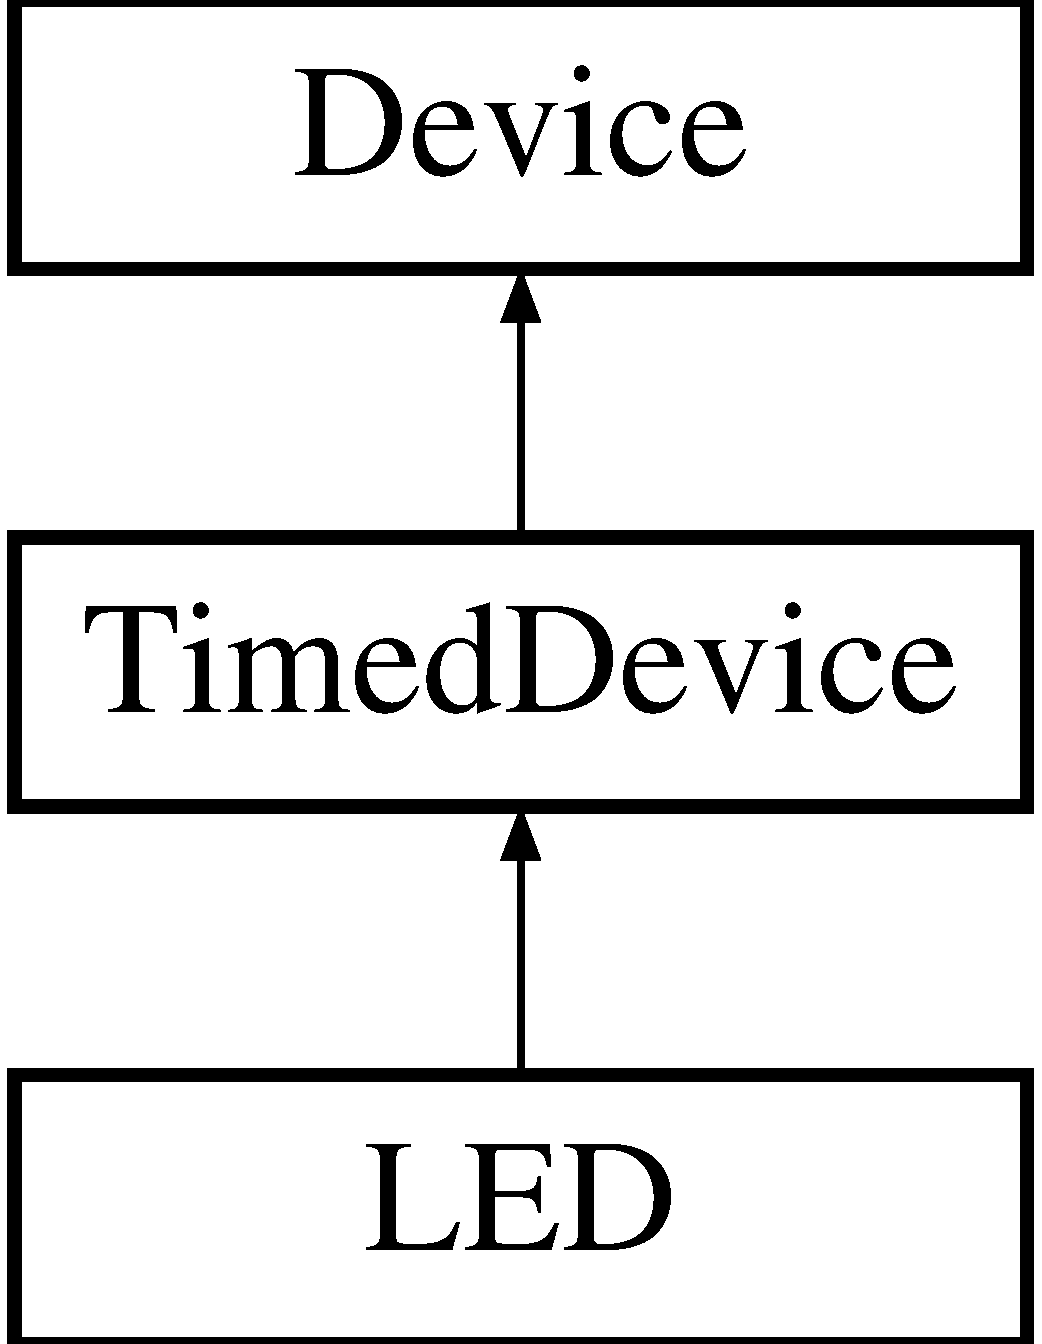
\includegraphics[height=3.000000cm]{classTimedDevice}
\end{center}
\end{figure}
\subsection*{Métodos Públicos}
\begin{DoxyCompactItemize}
\item 
\hyperlink{classTimedDevice_a5c428c52a02ae995463711400244cb1e}{Timed\-Device} (bool \hyperlink{classDevice_a463598bce318556c79bfc0f26b38f7d3}{is\-Effector}, bool \hyperlink{classDevice_a848bce229a669a4e7531bce2b6b24154}{is\-Sensor}=false)
\end{DoxyCompactItemize}
\subsection*{Atributos Estáticos Protegidos}
\begin{DoxyCompactItemize}
\item 
static \hyperlink{classClock}{Clock} \& \hyperlink{classTimedDevice_ab7a7601ea3e4ecea7a388d9216c67aaf}{clock} = Robot\-::clock
\end{DoxyCompactItemize}


\subsection{Construtores \& Destrutores}
\hypertarget{classTimedDevice_a5c428c52a02ae995463711400244cb1e}{\index{Timed\-Device@{Timed\-Device}!Timed\-Device@{Timed\-Device}}
\index{Timed\-Device@{Timed\-Device}!TimedDevice@{Timed\-Device}}
\subsubsection[{Timed\-Device}]{\setlength{\rightskip}{0pt plus 5cm}Timed\-Device\-::\-Timed\-Device (
\begin{DoxyParamCaption}
\item[{bool}]{is\-Effector, }
\item[{bool}]{is\-Sensor = {\ttfamily false}}
\end{DoxyParamCaption}
)\hspace{0.3cm}{\ttfamily [inline]}}}\label{classTimedDevice_a5c428c52a02ae995463711400244cb1e}


\subsection{Atributos}
\hypertarget{classTimedDevice_ab7a7601ea3e4ecea7a388d9216c67aaf}{\index{Timed\-Device@{Timed\-Device}!clock@{clock}}
\index{clock@{clock}!TimedDevice@{Timed\-Device}}
\subsubsection[{clock}]{\setlength{\rightskip}{0pt plus 5cm}{\bf Clock} \& Timed\-Device\-::clock = Robot\-::clock\hspace{0.3cm}{\ttfamily [static]}, {\ttfamily [protected]}}}\label{classTimedDevice_ab7a7601ea3e4ecea7a388d9216c67aaf}


A documentação para esta classe foi gerada a partir dos seguintes arquivos\-:\begin{DoxyCompactItemize}
\item 
\hyperlink{Clock_8h}{Clock.\-h}\item 
\hyperlink{Clock_8cpp}{Clock.\-cpp}\end{DoxyCompactItemize}

\chapter{Arquivos}
\hypertarget{Clock_8cpp}{\section{Referência do Arquivo Clock.\-cpp}
\label{Clock_8cpp}\index{Clock.\-cpp@{Clock.\-cpp}}
}
{\ttfamily \#include \char`\"{}Clock.\-h\char`\"{}}\\*
{\ttfamily \#include \char`\"{}Robot.\-h\char`\"{}}\\*


\subsection{Descrição Detalhada}
\begin{DoxyAuthor}{Autor}
Anderson Antunes \href{mailto:anderson.utf@gmail.com}{\tt anderson.\-utf@gmail.\-com} 
\end{DoxyAuthor}
\begin{DoxyVersion}{Versão}
1.\-0
\end{DoxyVersion}
\hypertarget{SerialConnection_8h_LICENSE}{}\subsection{L\-I\-C\-E\-N\-S\-E}\label{SerialConnection_8h_LICENSE}
Copyright (C) 2013 by Anderson Antunes \href{mailto:anderson.utf@gmail.com}{\tt anderson.\-utf@gmail.\-com}

Robot\-Lib is free software\-: you can redistribute it and/or modify it under the terms of the G\-N\-U General Public License as published by the Free Software Foundation, either version 3 of the License, or (at your option) any later version.

Robot\-Lib is distributed in the hope that it will be useful, but W\-I\-T\-H\-O\-U\-T A\-N\-Y W\-A\-R\-R\-A\-N\-T\-Y; without even the implied warranty of M\-E\-R\-C\-H\-A\-N\-T\-A\-B\-I\-L\-I\-T\-Y or F\-I\-T\-N\-E\-S\-S F\-O\-R A P\-A\-R\-T\-I\-C\-U\-L\-A\-R P\-U\-R\-P\-O\-S\-E. See the G\-N\-U General Public License for more details.

You should have received a copy of the G\-N\-U General Public License along with Robot\-Lib. If not, see \href{http://www.gnu.org/licenses/}{\tt http\-://www.\-gnu.\-org/licenses/}. 
\hypertarget{Clock_8h}{\section{Referência do Arquivo Clock.\-h}
\label{Clock_8h}\index{Clock.\-h@{Clock.\-h}}
}
{\ttfamily \#include $<$stdint.\-h$>$}\\*
{\ttfamily \#include $<$Arduino.\-h$>$}\\*
{\ttfamily \#include \char`\"{}Debug.\-h\char`\"{}}\\*
{\ttfamily \#include \char`\"{}Device.\-h\char`\"{}}\\*
\subsection*{Componentes}
\begin{DoxyCompactItemize}
\item 
class \hyperlink{classClock}{Clock}
\item 
class \hyperlink{classTimedDevice}{Timed\-Device}
\end{DoxyCompactItemize}
\subsection*{Definições de Tipos}
\begin{DoxyCompactItemize}
\item 
typedef int16\-\_\-t \hyperlink{Clock_8h_ae646ae1606f53892b8112edd8f8ab903}{Timer}
\end{DoxyCompactItemize}


\subsection{Descrição Detalhada}
\begin{DoxyAuthor}{Autor}
Anderson Antunes \href{mailto:anderson.utf@gmail.com}{\tt anderson.\-utf@gmail.\-com} 
\end{DoxyAuthor}
\begin{DoxyVersion}{Versão}
1.\-0
\end{DoxyVersion}
\hypertarget{SerialConnection_8h_LICENSE}{}\subsection{L\-I\-C\-E\-N\-S\-E}\label{SerialConnection_8h_LICENSE}
Copyright (C) 2013 by Anderson Antunes \href{mailto:anderson.utf@gmail.com}{\tt anderson.\-utf@gmail.\-com}

Robot\-Lib is free software\-: you can redistribute it and/or modify it under the terms of the G\-N\-U General Public License as published by the Free Software Foundation, either version 3 of the License, or (at your option) any later version.

Robot\-Lib is distributed in the hope that it will be useful, but W\-I\-T\-H\-O\-U\-T A\-N\-Y W\-A\-R\-R\-A\-N\-T\-Y; without even the implied warranty of M\-E\-R\-C\-H\-A\-N\-T\-A\-B\-I\-L\-I\-T\-Y or F\-I\-T\-N\-E\-S\-S F\-O\-R A P\-A\-R\-T\-I\-C\-U\-L\-A\-R P\-U\-R\-P\-O\-S\-E. See the G\-N\-U General Public License for more details.

You should have received a copy of the G\-N\-U General Public License along with Robot\-Lib. If not, see \href{http://www.gnu.org/licenses/}{\tt http\-://www.\-gnu.\-org/licenses/}. 

\subsection{Definições dos tipos}
\hypertarget{Clock_8h_ae646ae1606f53892b8112edd8f8ab903}{\index{Clock.\-h@{Clock.\-h}!Timer@{Timer}}
\index{Timer@{Timer}!Clock.h@{Clock.\-h}}
\subsubsection[{Timer}]{\setlength{\rightskip}{0pt plus 5cm}typedef int16\-\_\-t {\bf Timer}}}\label{Clock_8h_ae646ae1606f53892b8112edd8f8ab903}

\hypertarget{Compass_8cpp}{\section{Referência do Arquivo Compass.\-cpp}
\label{Compass_8cpp}\index{Compass.\-cpp@{Compass.\-cpp}}
}
{\ttfamily \#include $<$Arduino.\-h$>$}\\*
{\ttfamily \#include $<$Wire.\-h$>$}\\*
{\ttfamily \#include $<$H\-M\-C5883\-L.\-h$>$}\\*
{\ttfamily \#include \char`\"{}Compass.\-h\char`\"{}}\\*


\subsection{Descrição Detalhada}
\begin{DoxyAuthor}{Autor}
Diego Lee \href{mailto:diegolee7@gmail.com}{\tt diegolee7@gmail.\-com} 

Anderson Antunes \href{mailto:anderson.utf@gmail.com}{\tt anderson.\-utf@gmail.\-com} 
\end{DoxyAuthor}
\begin{DoxyVersion}{Versão}
1.\-0
\end{DoxyVersion}
\hypertarget{SerialConnection_8h_LICENSE}{}\subsection{L\-I\-C\-E\-N\-S\-E}\label{SerialConnection_8h_LICENSE}
Copyright (C) 2013 by Diego Lee \href{mailto:diegolee7@gmail.com}{\tt diegolee7@gmail.\-com} Anderson Antunes \href{mailto:anderson.utf@gmail.com}{\tt anderson.\-utf@gmail.\-com}

Robot\-Lib is free software\-: you can redistribute it and/or modify it under the terms of the G\-N\-U General Public License as published by the Free Software Foundation, either version 3 of the License, or (at your option) any later version.

Robot\-Lib is distributed in the hope that it will be useful, but W\-I\-T\-H\-O\-U\-T A\-N\-Y W\-A\-R\-R\-A\-N\-T\-Y; without even the implied warranty of M\-E\-R\-C\-H\-A\-N\-T\-A\-B\-I\-L\-I\-T\-Y or F\-I\-T\-N\-E\-S\-S F\-O\-R A P\-A\-R\-T\-I\-C\-U\-L\-A\-R P\-U\-R\-P\-O\-S\-E. See the G\-N\-U General Public License for more details.

You should have received a copy of the G\-N\-U General Public License along with Robot\-Lib. If not, see \href{http://www.gnu.org/licenses/}{\tt http\-://www.\-gnu.\-org/licenses/}. 
\hypertarget{Compass_8h}{\section{Referência do Arquivo Compass.\-h}
\label{Compass_8h}\index{Compass.\-h@{Compass.\-h}}
}
{\ttfamily \#include $<$stdint.\-h$>$}\\*
{\ttfamily \#include \char`\"{}../\-H\-M\-C5883\-L/\-H\-M\-C5883\-L.\-h\char`\"{}}\\*
{\ttfamily \#include \char`\"{}Device.\-h\char`\"{}}\\*
\subsection*{Componentes}
\begin{DoxyCompactItemize}
\item 
class \hyperlink{classCompass}{Compass}
\end{DoxyCompactItemize}


\subsection{Descrição Detalhada}
\begin{DoxyAuthor}{Autor}
Diego Lee \href{mailto:diegolee7@gmail.com}{\tt diegolee7@gmail.\-com} 

Anderson Antunes \href{mailto:anderson.utf@gmail.com}{\tt anderson.\-utf@gmail.\-com} 
\end{DoxyAuthor}
\begin{DoxyVersion}{Versão}
1.\-0
\end{DoxyVersion}
\hypertarget{SerialConnection_8h_LICENSE}{}\subsection{L\-I\-C\-E\-N\-S\-E}\label{SerialConnection_8h_LICENSE}
Copyright (C) 2013 by Diego Lee \href{mailto:diegolee7@gmail.com}{\tt diegolee7@gmail.\-com} Anderson Antunes \href{mailto:anderson.utf@gmail.com}{\tt anderson.\-utf@gmail.\-com}

Robot\-Lib is free software\-: you can redistribute it and/or modify it under the terms of the G\-N\-U General Public License as published by the Free Software Foundation, either version 3 of the License, or (at your option) any later version.

Robot\-Lib is distributed in the hope that it will be useful, but W\-I\-T\-H\-O\-U\-T A\-N\-Y W\-A\-R\-R\-A\-N\-T\-Y; without even the implied warranty of M\-E\-R\-C\-H\-A\-N\-T\-A\-B\-I\-L\-I\-T\-Y or F\-I\-T\-N\-E\-S\-S F\-O\-R A P\-A\-R\-T\-I\-C\-U\-L\-A\-R P\-U\-R\-P\-O\-S\-E. See the G\-N\-U General Public License for more details.

You should have received a copy of the G\-N\-U General Public License along with Robot\-Lib. If not, see \href{http://www.gnu.org/licenses/}{\tt http\-://www.\-gnu.\-org/licenses/}. 
\hypertarget{Connection_8h}{\section{Referência do Arquivo Connection.\-h}
\label{Connection_8h}\index{Connection.\-h@{Connection.\-h}}
}
{\ttfamily \#include $<$stdint.\-h$>$}\\*
\subsection*{Componentes}
\begin{DoxyCompactItemize}
\item 
class \hyperlink{classConnection}{Connection}
\end{DoxyCompactItemize}


\subsection{Descrição Detalhada}
\begin{DoxyAuthor}{Autor}
Anderson Antunes \href{mailto:anderson.utf@gmail.com}{\tt anderson.\-utf@gmail.\-com} 
\end{DoxyAuthor}
\begin{DoxyVersion}{Versão}
1.\-0
\end{DoxyVersion}
\hypertarget{SerialConnection_8h_LICENSE}{}\subsection{L\-I\-C\-E\-N\-S\-E}\label{SerialConnection_8h_LICENSE}
Copyright (C) 2013 by Anderson Antunes \href{mailto:anderson.utf@gmail.com}{\tt anderson.\-utf@gmail.\-com}

Robot\-Lib is free software\-: you can redistribute it and/or modify it under the terms of the G\-N\-U General Public License as published by the Free Software Foundation, either version 3 of the License, or (at your option) any later version.

Robot\-Lib is distributed in the hope that it will be useful, but W\-I\-T\-H\-O\-U\-T A\-N\-Y W\-A\-R\-R\-A\-N\-T\-Y; without even the implied warranty of M\-E\-R\-C\-H\-A\-N\-T\-A\-B\-I\-L\-I\-T\-Y or F\-I\-T\-N\-E\-S\-S F\-O\-R A P\-A\-R\-T\-I\-C\-U\-L\-A\-R P\-U\-R\-P\-O\-S\-E. See the G\-N\-U General Public License for more details.

You should have received a copy of the G\-N\-U General Public License along with Robot\-Lib. If not, see \href{http://www.gnu.org/licenses/}{\tt http\-://www.\-gnu.\-org/licenses/}. 
\hypertarget{Debug_8cpp}{\section{Referência do Arquivo Debug.\-cpp}
\label{Debug_8cpp}\index{Debug.\-cpp@{Debug.\-cpp}}
}
{\ttfamily \#include \char`\"{}Debug.\-h\char`\"{}}\\*
\subsection*{Definições e Macros}
\begin{DoxyCompactItemize}
\item 
\#define \hyperlink{Debug_8cpp_aeb7a7ba1ab7e0406f1b5ab36d579f585}{L\-E\-D}~3
\item 
\#define \hyperlink{Debug_8cpp_a99bef6dff19479278b00d124a469e667}{M\-A\-X\-\_\-\-D\-E\-L\-A\-Y\-\_\-\-E\-R\-R\-O\-R}~80
\item 
\#define \hyperlink{Debug_8cpp_aef1b2b011378477dc1631b453f964b05}{M\-I\-N\-\_\-\-D\-E\-L\-A\-Y\-\_\-\-E\-R\-R\-O\-R}~20
\end{DoxyCompactItemize}
\subsection*{Funções}
\begin{DoxyCompactItemize}
\item 
void \hyperlink{Debug_8cpp_aae9d52caad9fb2892deeb25596cfd2ab}{kill} ()
\begin{DoxyCompactList}\small\item\em Desativa o robô enviando uma sequência predefinida para o \hyperlink{classLED}{L\-E\-D} de debug em um loop infinito. \end{DoxyCompactList}\item 
void $\ast$ \hyperlink{Debug_8cpp_a44004265ee55099761200d8956b600e8}{check} (void $\ast$p)
\begin{DoxyCompactList}\small\item\em Verifica de o ponteiro {\ttfamily p} é válido, caso contrário executa {\ttfamily kill}. \end{DoxyCompactList}\item 
void \hyperlink{Debug_8cpp_a39ad5f2cf0013ae6eca89f0c8ebfcbb6}{blink} (int n, int pulse\-\_\-time)
\begin{DoxyCompactList}\small\item\em Pisca o \hyperlink{classLED}{L\-E\-D} de debug {\ttfamily n} vezes por {\ttfamily pulse\-\_\-time} ms. \end{DoxyCompactList}\item 
int \hyperlink{Debug_8cpp_aac7b29dc45caaaca67299571f6a2dcc0}{free\-Ram} ()
\begin{DoxyCompactList}\small\item\em Retorna a quantidade de memoria R\-A\-M disponível. \end{DoxyCompactList}\end{DoxyCompactItemize}


\subsection{Descrição Detalhada}
\begin{DoxyAuthor}{Autor}
Anderson Antunes \href{mailto:anderson.utf@gmail.com}{\tt anderson.\-utf@gmail.\-com} 
\end{DoxyAuthor}
\begin{DoxyVersion}{Versão}
1.\-0
\end{DoxyVersion}
\hypertarget{SerialConnection_8h_LICENSE}{}\subsection{L\-I\-C\-E\-N\-S\-E}\label{SerialConnection_8h_LICENSE}
Copyright (C) 2013 by Anderson Antunes \href{mailto:anderson.utf@gmail.com}{\tt anderson.\-utf@gmail.\-com}

Robot\-Lib is free software\-: you can redistribute it and/or modify it under the terms of the G\-N\-U General Public License as published by the Free Software Foundation, either version 3 of the License, or (at your option) any later version.

Robot\-Lib is distributed in the hope that it will be useful, but W\-I\-T\-H\-O\-U\-T A\-N\-Y W\-A\-R\-R\-A\-N\-T\-Y; without even the implied warranty of M\-E\-R\-C\-H\-A\-N\-T\-A\-B\-I\-L\-I\-T\-Y or F\-I\-T\-N\-E\-S\-S F\-O\-R A P\-A\-R\-T\-I\-C\-U\-L\-A\-R P\-U\-R\-P\-O\-S\-E. See the G\-N\-U General Public License for more details.

You should have received a copy of the G\-N\-U General Public License along with Robot\-Lib. If not, see \href{http://www.gnu.org/licenses/}{\tt http\-://www.\-gnu.\-org/licenses/}.\hypertarget{Debug_8h_DESCRIPTION}{}\subsection{D\-E\-S\-C\-R\-I\-P\-T\-I\-O\-N}\label{Debug_8h_DESCRIPTION}
Conjunto de funções para debug. 

\subsection{Definições e macros}
\hypertarget{Debug_8cpp_aeb7a7ba1ab7e0406f1b5ab36d579f585}{\index{Debug.\-cpp@{Debug.\-cpp}!L\-E\-D@{L\-E\-D}}
\index{L\-E\-D@{L\-E\-D}!Debug.cpp@{Debug.\-cpp}}
\subsubsection[{L\-E\-D}]{\setlength{\rightskip}{0pt plus 5cm}\#define {\bf L\-E\-D}~3}}\label{Debug_8cpp_aeb7a7ba1ab7e0406f1b5ab36d579f585}
\hypertarget{Debug_8cpp_a99bef6dff19479278b00d124a469e667}{\index{Debug.\-cpp@{Debug.\-cpp}!M\-A\-X\-\_\-\-D\-E\-L\-A\-Y\-\_\-\-E\-R\-R\-O\-R@{M\-A\-X\-\_\-\-D\-E\-L\-A\-Y\-\_\-\-E\-R\-R\-O\-R}}
\index{M\-A\-X\-\_\-\-D\-E\-L\-A\-Y\-\_\-\-E\-R\-R\-O\-R@{M\-A\-X\-\_\-\-D\-E\-L\-A\-Y\-\_\-\-E\-R\-R\-O\-R}!Debug.cpp@{Debug.\-cpp}}
\subsubsection[{M\-A\-X\-\_\-\-D\-E\-L\-A\-Y\-\_\-\-E\-R\-R\-O\-R}]{\setlength{\rightskip}{0pt plus 5cm}\#define M\-A\-X\-\_\-\-D\-E\-L\-A\-Y\-\_\-\-E\-R\-R\-O\-R~80}}\label{Debug_8cpp_a99bef6dff19479278b00d124a469e667}
\hypertarget{Debug_8cpp_aef1b2b011378477dc1631b453f964b05}{\index{Debug.\-cpp@{Debug.\-cpp}!M\-I\-N\-\_\-\-D\-E\-L\-A\-Y\-\_\-\-E\-R\-R\-O\-R@{M\-I\-N\-\_\-\-D\-E\-L\-A\-Y\-\_\-\-E\-R\-R\-O\-R}}
\index{M\-I\-N\-\_\-\-D\-E\-L\-A\-Y\-\_\-\-E\-R\-R\-O\-R@{M\-I\-N\-\_\-\-D\-E\-L\-A\-Y\-\_\-\-E\-R\-R\-O\-R}!Debug.cpp@{Debug.\-cpp}}
\subsubsection[{M\-I\-N\-\_\-\-D\-E\-L\-A\-Y\-\_\-\-E\-R\-R\-O\-R}]{\setlength{\rightskip}{0pt plus 5cm}\#define M\-I\-N\-\_\-\-D\-E\-L\-A\-Y\-\_\-\-E\-R\-R\-O\-R~20}}\label{Debug_8cpp_aef1b2b011378477dc1631b453f964b05}


\subsection{Funções}
\hypertarget{Debug_8cpp_a39ad5f2cf0013ae6eca89f0c8ebfcbb6}{\index{Debug.\-cpp@{Debug.\-cpp}!blink@{blink}}
\index{blink@{blink}!Debug.cpp@{Debug.\-cpp}}
\subsubsection[{blink}]{\setlength{\rightskip}{0pt plus 5cm}void blink (
\begin{DoxyParamCaption}
\item[{int}]{n, }
\item[{int}]{pulse\-\_\-time}
\end{DoxyParamCaption}
)}}\label{Debug_8cpp_a39ad5f2cf0013ae6eca89f0c8ebfcbb6}


Pisca o \hyperlink{classLED}{L\-E\-D} de debug {\ttfamily n} vezes por {\ttfamily pulse\-\_\-time} ms. 


\begin{DoxyParams}{Parâmetros}
{\em n} & Número de vezes que o \hyperlink{classLED}{L\-E\-D} deverá piscar. \\
\hline
{\em pulse\-\_\-time} & Tempo em ms de cada pulso do \hyperlink{classLED}{L\-E\-D}. \\
\hline
\end{DoxyParams}
\hypertarget{Debug_8cpp_a44004265ee55099761200d8956b600e8}{\index{Debug.\-cpp@{Debug.\-cpp}!check@{check}}
\index{check@{check}!Debug.cpp@{Debug.\-cpp}}
\subsubsection[{check}]{\setlength{\rightskip}{0pt plus 5cm}void$\ast$ check (
\begin{DoxyParamCaption}
\item[{void $\ast$}]{p}
\end{DoxyParamCaption}
)}}\label{Debug_8cpp_a44004265ee55099761200d8956b600e8}


Verifica de o ponteiro {\ttfamily p} é válido, caso contrário executa {\ttfamily kill}. 


\begin{DoxyParams}[1]{Parâmetros}
\mbox{\tt in}  & {\em p} & Um ponteiro qualquer. \\
\hline
\end{DoxyParams}
\hypertarget{Debug_8cpp_aac7b29dc45caaaca67299571f6a2dcc0}{\index{Debug.\-cpp@{Debug.\-cpp}!free\-Ram@{free\-Ram}}
\index{free\-Ram@{free\-Ram}!Debug.cpp@{Debug.\-cpp}}
\subsubsection[{free\-Ram}]{\setlength{\rightskip}{0pt plus 5cm}int free\-Ram (
\begin{DoxyParamCaption}
{}
\end{DoxyParamCaption}
)}}\label{Debug_8cpp_aac7b29dc45caaaca67299571f6a2dcc0}


Retorna a quantidade de memoria R\-A\-M disponível. 

\begin{DoxyReturn}{Retorna}
o número de bytes disponíveis. 
\end{DoxyReturn}
\hypertarget{Debug_8cpp_aae9d52caad9fb2892deeb25596cfd2ab}{\index{Debug.\-cpp@{Debug.\-cpp}!kill@{kill}}
\index{kill@{kill}!Debug.cpp@{Debug.\-cpp}}
\subsubsection[{kill}]{\setlength{\rightskip}{0pt plus 5cm}void kill (
\begin{DoxyParamCaption}
{}
\end{DoxyParamCaption}
)}}\label{Debug_8cpp_aae9d52caad9fb2892deeb25596cfd2ab}


Desativa o robô enviando uma sequência predefinida para o \hyperlink{classLED}{L\-E\-D} de debug em um loop infinito. 


\hypertarget{Debug_8h}{\section{Referência do Arquivo Debug.\-h}
\label{Debug_8h}\index{Debug.\-h@{Debug.\-h}}
}
{\ttfamily \#include $<$Arduino.\-h$>$}\\*
{\ttfamily \#include $<$avr/wdt.\-h$>$}\\*
\subsection*{Definições e Macros}
\begin{DoxyCompactItemize}
\item 
\#define \hyperlink{Debug_8h_a4b86784c25c7fd1b5ae95ddf5831254a}{Reset\-\_\-\-A\-V\-R}()~wdt\-\_\-enable(W\-D\-T\-O\-\_\-30\-M\-S); while(1) \{\}
\begin{DoxyCompactList}\small\item\em Reseta o microcontrolador;. \end{DoxyCompactList}\end{DoxyCompactItemize}
\subsection*{Funções}
\begin{DoxyCompactItemize}
\item 
void \hyperlink{Debug_8h_aae9d52caad9fb2892deeb25596cfd2ab}{kill} ()
\begin{DoxyCompactList}\small\item\em Desativa o robô enviando uma sequência predefinida para o \hyperlink{classLED}{L\-E\-D} de debug em um loop infinito. \end{DoxyCompactList}\item 
void $\ast$ \hyperlink{Debug_8h_a44004265ee55099761200d8956b600e8}{check} (void $\ast$p)
\begin{DoxyCompactList}\small\item\em Verifica de o ponteiro {\ttfamily p} é válido, caso contrário executa {\ttfamily kill}. \end{DoxyCompactList}\item 
void \hyperlink{Debug_8h_a39ad5f2cf0013ae6eca89f0c8ebfcbb6}{blink} (int n, int pulse\-\_\-time)
\begin{DoxyCompactList}\small\item\em Pisca o \hyperlink{classLED}{L\-E\-D} de debug {\ttfamily n} vezes por {\ttfamily pulse\-\_\-time} ms. \end{DoxyCompactList}\item 
int \hyperlink{Debug_8h_aac7b29dc45caaaca67299571f6a2dcc0}{free\-Ram} ()
\begin{DoxyCompactList}\small\item\em Retorna a quantidade de memoria R\-A\-M disponível. \end{DoxyCompactList}\end{DoxyCompactItemize}


\subsection{Descrição Detalhada}
\begin{DoxyAuthor}{Autor}
Anderson Antunes \href{mailto:anderson.utf@gmail.com}{\tt anderson.\-utf@gmail.\-com} 
\end{DoxyAuthor}
\begin{DoxyVersion}{Versão}
1.\-0
\end{DoxyVersion}
\hypertarget{SerialConnection_8h_LICENSE}{}\subsection{L\-I\-C\-E\-N\-S\-E}\label{SerialConnection_8h_LICENSE}
Copyright (C) 2013 by Anderson Antunes \href{mailto:anderson.utf@gmail.com}{\tt anderson.\-utf@gmail.\-com}

Robot\-Lib is free software\-: you can redistribute it and/or modify it under the terms of the G\-N\-U General Public License as published by the Free Software Foundation, either version 3 of the License, or (at your option) any later version.

Robot\-Lib is distributed in the hope that it will be useful, but W\-I\-T\-H\-O\-U\-T A\-N\-Y W\-A\-R\-R\-A\-N\-T\-Y; without even the implied warranty of M\-E\-R\-C\-H\-A\-N\-T\-A\-B\-I\-L\-I\-T\-Y or F\-I\-T\-N\-E\-S\-S F\-O\-R A P\-A\-R\-T\-I\-C\-U\-L\-A\-R P\-U\-R\-P\-O\-S\-E. See the G\-N\-U General Public License for more details.

You should have received a copy of the G\-N\-U General Public License along with Robot\-Lib. If not, see \href{http://www.gnu.org/licenses/}{\tt http\-://www.\-gnu.\-org/licenses/}.\hypertarget{Debug_8h_DESCRIPTION}{}\subsection{D\-E\-S\-C\-R\-I\-P\-T\-I\-O\-N}\label{Debug_8h_DESCRIPTION}
Conjunto de funções para debug. 

\subsection{Definições e macros}
\hypertarget{Debug_8h_a4b86784c25c7fd1b5ae95ddf5831254a}{\index{Debug.\-h@{Debug.\-h}!Reset\-\_\-\-A\-V\-R@{Reset\-\_\-\-A\-V\-R}}
\index{Reset\-\_\-\-A\-V\-R@{Reset\-\_\-\-A\-V\-R}!Debug.h@{Debug.\-h}}
\subsubsection[{Reset\-\_\-\-A\-V\-R}]{\setlength{\rightskip}{0pt plus 5cm}\#define Reset\-\_\-\-A\-V\-R(
\begin{DoxyParamCaption}
{}
\end{DoxyParamCaption}
)~wdt\-\_\-enable(W\-D\-T\-O\-\_\-30\-M\-S); while(1) \{\}}}\label{Debug_8h_a4b86784c25c7fd1b5ae95ddf5831254a}


Reseta o microcontrolador;. 



\subsection{Funções}
\hypertarget{Debug_8h_a39ad5f2cf0013ae6eca89f0c8ebfcbb6}{\index{Debug.\-h@{Debug.\-h}!blink@{blink}}
\index{blink@{blink}!Debug.h@{Debug.\-h}}
\subsubsection[{blink}]{\setlength{\rightskip}{0pt plus 5cm}void blink (
\begin{DoxyParamCaption}
\item[{int}]{n, }
\item[{int}]{pulse\-\_\-time}
\end{DoxyParamCaption}
)}}\label{Debug_8h_a39ad5f2cf0013ae6eca89f0c8ebfcbb6}


Pisca o \hyperlink{classLED}{L\-E\-D} de debug {\ttfamily n} vezes por {\ttfamily pulse\-\_\-time} ms. 


\begin{DoxyParams}{Parâmetros}
{\em n} & Número de vezes que o \hyperlink{classLED}{L\-E\-D} deverá piscar. \\
\hline
{\em pulse\-\_\-time} & Tempo em ms de cada pulso do \hyperlink{classLED}{L\-E\-D}. \\
\hline
\end{DoxyParams}
\hypertarget{Debug_8h_a44004265ee55099761200d8956b600e8}{\index{Debug.\-h@{Debug.\-h}!check@{check}}
\index{check@{check}!Debug.h@{Debug.\-h}}
\subsubsection[{check}]{\setlength{\rightskip}{0pt plus 5cm}void$\ast$ check (
\begin{DoxyParamCaption}
\item[{void $\ast$}]{p}
\end{DoxyParamCaption}
)}}\label{Debug_8h_a44004265ee55099761200d8956b600e8}


Verifica de o ponteiro {\ttfamily p} é válido, caso contrário executa {\ttfamily kill}. 


\begin{DoxyParams}[1]{Parâmetros}
\mbox{\tt in}  & {\em p} & Um ponteiro qualquer. \\
\hline
\end{DoxyParams}
\hypertarget{Debug_8h_aac7b29dc45caaaca67299571f6a2dcc0}{\index{Debug.\-h@{Debug.\-h}!free\-Ram@{free\-Ram}}
\index{free\-Ram@{free\-Ram}!Debug.h@{Debug.\-h}}
\subsubsection[{free\-Ram}]{\setlength{\rightskip}{0pt plus 5cm}int free\-Ram (
\begin{DoxyParamCaption}
{}
\end{DoxyParamCaption}
)}}\label{Debug_8h_aac7b29dc45caaaca67299571f6a2dcc0}


Retorna a quantidade de memoria R\-A\-M disponível. 

\begin{DoxyReturn}{Retorna}
o número de bytes disponíveis. 
\end{DoxyReturn}
\hypertarget{Debug_8h_aae9d52caad9fb2892deeb25596cfd2ab}{\index{Debug.\-h@{Debug.\-h}!kill@{kill}}
\index{kill@{kill}!Debug.h@{Debug.\-h}}
\subsubsection[{kill}]{\setlength{\rightskip}{0pt plus 5cm}void kill (
\begin{DoxyParamCaption}
{}
\end{DoxyParamCaption}
)}}\label{Debug_8h_aae9d52caad9fb2892deeb25596cfd2ab}


Desativa o robô enviando uma sequência predefinida para o \hyperlink{classLED}{L\-E\-D} de debug em um loop infinito. 


\hypertarget{Device_8cpp}{\section{Referência do Arquivo Device.\-cpp}
\label{Device_8cpp}\index{Device.\-cpp@{Device.\-cpp}}
}
{\ttfamily \#include \char`\"{}Device.\-h\char`\"{}}\\*


\subsection{Descrição Detalhada}
\begin{DoxyAuthor}{Autor}
Anderson Antunes \href{mailto:anderson.utf@gmail.com}{\tt anderson.\-utf@gmail.\-com} 
\end{DoxyAuthor}
\begin{DoxyVersion}{Versão}
1.\-0
\end{DoxyVersion}
\hypertarget{SerialConnection_8h_LICENSE}{}\subsection{L\-I\-C\-E\-N\-S\-E}\label{SerialConnection_8h_LICENSE}
Copyright (C) 2013 by Anderson Antunes \href{mailto:anderson.utf@gmail.com}{\tt anderson.\-utf@gmail.\-com}

Robot\-Lib is free software\-: you can redistribute it and/or modify it under the terms of the G\-N\-U General Public License as published by the Free Software Foundation, either version 3 of the License, or (at your option) any later version.

Robot\-Lib is distributed in the hope that it will be useful, but W\-I\-T\-H\-O\-U\-T A\-N\-Y W\-A\-R\-R\-A\-N\-T\-Y; without even the implied warranty of M\-E\-R\-C\-H\-A\-N\-T\-A\-B\-I\-L\-I\-T\-Y or F\-I\-T\-N\-E\-S\-S F\-O\-R A P\-A\-R\-T\-I\-C\-U\-L\-A\-R P\-U\-R\-P\-O\-S\-E. See the G\-N\-U General Public License for more details.

You should have received a copy of the G\-N\-U General Public License along with Robot\-Lib. If not, see \href{http://www.gnu.org/licenses/}{\tt http\-://www.\-gnu.\-org/licenses/}. 
\hypertarget{Device_8h}{\section{Referência do Arquivo Device.\-h}
\label{Device_8h}\index{Device.\-h@{Device.\-h}}
}
{\ttfamily \#include $<$stdint.\-h$>$}\\*
\subsection*{Componentes}
\begin{DoxyCompactItemize}
\item 
class \hyperlink{classDevice}{Device}
\end{DoxyCompactItemize}


\subsection{Descrição Detalhada}
\begin{DoxyAuthor}{Autor}
Anderson Antunes \href{mailto:anderson.utf@gmail.com}{\tt anderson.\-utf@gmail.\-com} 
\end{DoxyAuthor}
\begin{DoxyVersion}{Versão}
1.\-0
\end{DoxyVersion}
\hypertarget{SerialConnection_8h_LICENSE}{}\subsection{L\-I\-C\-E\-N\-S\-E}\label{SerialConnection_8h_LICENSE}
Copyright (C) 2013 by Anderson Antunes \href{mailto:anderson.utf@gmail.com}{\tt anderson.\-utf@gmail.\-com}

Robot\-Lib is free software\-: you can redistribute it and/or modify it under the terms of the G\-N\-U General Public License as published by the Free Software Foundation, either version 3 of the License, or (at your option) any later version.

Robot\-Lib is distributed in the hope that it will be useful, but W\-I\-T\-H\-O\-U\-T A\-N\-Y W\-A\-R\-R\-A\-N\-T\-Y; without even the implied warranty of M\-E\-R\-C\-H\-A\-N\-T\-A\-B\-I\-L\-I\-T\-Y or F\-I\-T\-N\-E\-S\-S F\-O\-R A P\-A\-R\-T\-I\-C\-U\-L\-A\-R P\-U\-R\-P\-O\-S\-E. See the G\-N\-U General Public License for more details.

You should have received a copy of the G\-N\-U General Public License along with Robot\-Lib. If not, see \href{http://www.gnu.org/licenses/}{\tt http\-://www.\-gnu.\-org/licenses/}. 
\hypertarget{Distance_8cpp}{\section{Referência do Arquivo Distance.\-cpp}
\label{Distance_8cpp}\index{Distance.\-cpp@{Distance.\-cpp}}
}
{\ttfamily \#include \char`\"{}Distance.\-h\char`\"{}}\\*

\hypertarget{Distance_8h}{\section{Referência do Arquivo Distance.\-h}
\label{Distance_8h}\index{Distance.\-h@{Distance.\-h}}
}
{\ttfamily \#include $<$stdint.\-h$>$}\\*
{\ttfamily \#include $<$Arduino.\-h$>$}\\*
{\ttfamily \#include \char`\"{}Device.\-h\char`\"{}}\\*
{\ttfamily \#include \char`\"{}Debug.\-h\char`\"{}}\\*
\subsection*{Componentes}
\begin{DoxyCompactItemize}
\item 
class \hyperlink{classDistance}{Distance}
\end{DoxyCompactItemize}

\hypertarget{GenericRobot_8cpp}{\section{Referência do Arquivo Generic\-Robot.\-cpp}
\label{GenericRobot_8cpp}\index{Generic\-Robot.\-cpp@{Generic\-Robot.\-cpp}}
}
{\ttfamily \#include \char`\"{}Generic\-Robot.\-h\char`\"{}}\\*
{\ttfamily \#include \char`\"{}L\-E\-D.\-h\char`\"{}}\\*
{\ttfamily \#include \char`\"{}H\-Bridge.\-h\char`\"{}}\\*
{\ttfamily \#include \char`\"{}Compass.\-h\char`\"{}}\\*
{\ttfamily \#include \char`\"{}Reflectance\-Sensor\-Array.\-h\char`\"{}}\\*
{\ttfamily \#include \char`\"{}I\-R\-Proximity\-Sensor.\-h\char`\"{}}\\*


\subsection{Descrição Detalhada}
\begin{DoxyAuthor}{Autor}
Anderson Antunes \href{mailto:anderson.utf@gmail.com}{\tt anderson.\-utf@gmail.\-com} 
\end{DoxyAuthor}
\begin{DoxyVersion}{Versão}
1.\-0
\end{DoxyVersion}
\hypertarget{SerialConnection_8h_LICENSE}{}\subsection{L\-I\-C\-E\-N\-S\-E}\label{SerialConnection_8h_LICENSE}
Copyright (C) 2013 by Anderson Antunes \href{mailto:anderson.utf@gmail.com}{\tt anderson.\-utf@gmail.\-com}

Robot\-Lib is free software\-: you can redistribute it and/or modify it under the terms of the G\-N\-U General Public License as published by the Free Software Foundation, either version 3 of the License, or (at your option) any later version.

Robot\-Lib is distributed in the hope that it will be useful, but W\-I\-T\-H\-O\-U\-T A\-N\-Y W\-A\-R\-R\-A\-N\-T\-Y; without even the implied warranty of M\-E\-R\-C\-H\-A\-N\-T\-A\-B\-I\-L\-I\-T\-Y or F\-I\-T\-N\-E\-S\-S F\-O\-R A P\-A\-R\-T\-I\-C\-U\-L\-A\-R P\-U\-R\-P\-O\-S\-E. See the G\-N\-U General Public License for more details.

You should have received a copy of the G\-N\-U General Public License along with Robot\-Lib. If not, see \href{http://www.gnu.org/licenses/}{\tt http\-://www.\-gnu.\-org/licenses/}. 
\hypertarget{GenericRobot_8h}{\section{Referência do Arquivo Generic\-Robot.\-h}
\label{GenericRobot_8h}\index{Generic\-Robot.\-h@{Generic\-Robot.\-h}}
}
{\ttfamily \#include $<$stdint.\-h$>$}\\*
{\ttfamily \#include \char`\"{}Radio\-Robot.\-h\char`\"{}}\\*
\subsection*{Componentes}
\begin{DoxyCompactItemize}
\item 
class \hyperlink{classGenericRobot}{Generic\-Robot}
\end{DoxyCompactItemize}
\subsection*{Enumerações}
\begin{DoxyCompactItemize}
\item 
enum \hyperlink{GenericRobot_8h_a833b28f90e109607cd5d9e826474893a}{D\-E\-V\-I\-C\-E} \{ \\*
\hyperlink{GenericRobot_8h_a833b28f90e109607cd5d9e826474893aa89e3c46d1f7e075c0bf8b665837fe13f}{D\-E\-V\-\_\-\-L\-E\-D} = 1, 
\hyperlink{GenericRobot_8h_a833b28f90e109607cd5d9e826474893aa60cc4333f7f6678b5e00fcc9c50a1dc2}{D\-E\-V\-\_\-\-H\-B\-R\-I\-D\-G\-E}, 
\hyperlink{GenericRobot_8h_a833b28f90e109607cd5d9e826474893aafea4c4bc3d9d0fa0b4859736368bad60}{D\-E\-V\-\_\-\-C\-O\-M\-P\-A\-S\-S}, 
\hyperlink{GenericRobot_8h_a833b28f90e109607cd5d9e826474893aa617f3892facbc92bb847da4b71c568dd}{D\-E\-V\-\_\-\-R\-E\-F\-L\-E\-C\-T}, 
\\*
\hyperlink{GenericRobot_8h_a833b28f90e109607cd5d9e826474893aa3712363d72b9d3f0af59fa19ed41c0eb}{D\-E\-V\-\_\-\-P\-R\-O\-X}
 \}
\end{DoxyCompactItemize}


\subsection{Descrição Detalhada}
\begin{DoxyAuthor}{Autor}
Anderson Antunes \href{mailto:anderson.utf@gmail.com}{\tt anderson.\-utf@gmail.\-com} 
\end{DoxyAuthor}
\begin{DoxyVersion}{Versão}
1.\-0
\end{DoxyVersion}
\hypertarget{SerialConnection_8h_LICENSE}{}\subsection{L\-I\-C\-E\-N\-S\-E}\label{SerialConnection_8h_LICENSE}
Copyright (C) 2013 by Anderson Antunes \href{mailto:anderson.utf@gmail.com}{\tt anderson.\-utf@gmail.\-com}

Robot\-Lib is free software\-: you can redistribute it and/or modify it under the terms of the G\-N\-U General Public License as published by the Free Software Foundation, either version 3 of the License, or (at your option) any later version.

Robot\-Lib is distributed in the hope that it will be useful, but W\-I\-T\-H\-O\-U\-T A\-N\-Y W\-A\-R\-R\-A\-N\-T\-Y; without even the implied warranty of M\-E\-R\-C\-H\-A\-N\-T\-A\-B\-I\-L\-I\-T\-Y or F\-I\-T\-N\-E\-S\-S F\-O\-R A P\-A\-R\-T\-I\-C\-U\-L\-A\-R P\-U\-R\-P\-O\-S\-E. See the G\-N\-U General Public License for more details.

You should have received a copy of the G\-N\-U General Public License along with Robot\-Lib. If not, see \href{http://www.gnu.org/licenses/}{\tt http\-://www.\-gnu.\-org/licenses/}. 

\subsection{Enumerações}
\hypertarget{GenericRobot_8h_a833b28f90e109607cd5d9e826474893a}{\index{Generic\-Robot.\-h@{Generic\-Robot.\-h}!D\-E\-V\-I\-C\-E@{D\-E\-V\-I\-C\-E}}
\index{D\-E\-V\-I\-C\-E@{D\-E\-V\-I\-C\-E}!GenericRobot.h@{Generic\-Robot.\-h}}
\subsubsection[{D\-E\-V\-I\-C\-E}]{\setlength{\rightskip}{0pt plus 5cm}enum {\bf D\-E\-V\-I\-C\-E}}}\label{GenericRobot_8h_a833b28f90e109607cd5d9e826474893a}
\begin{Desc}
\item[Valores enumerados\-: ]\par
\begin{description}
\index{D\-E\-V\-\_\-\-L\-E\-D@{D\-E\-V\-\_\-\-L\-E\-D}!Generic\-Robot.\-h@{Generic\-Robot.\-h}}\index{Generic\-Robot.\-h@{Generic\-Robot.\-h}!D\-E\-V\-\_\-\-L\-E\-D@{D\-E\-V\-\_\-\-L\-E\-D}}\item[{\em 
\hypertarget{GenericRobot_8h_a833b28f90e109607cd5d9e826474893aa89e3c46d1f7e075c0bf8b665837fe13f}{D\-E\-V\-\_\-\-L\-E\-D}\label{GenericRobot_8h_a833b28f90e109607cd5d9e826474893aa89e3c46d1f7e075c0bf8b665837fe13f}
}]\index{D\-E\-V\-\_\-\-H\-B\-R\-I\-D\-G\-E@{D\-E\-V\-\_\-\-H\-B\-R\-I\-D\-G\-E}!Generic\-Robot.\-h@{Generic\-Robot.\-h}}\index{Generic\-Robot.\-h@{Generic\-Robot.\-h}!D\-E\-V\-\_\-\-H\-B\-R\-I\-D\-G\-E@{D\-E\-V\-\_\-\-H\-B\-R\-I\-D\-G\-E}}\item[{\em 
\hypertarget{GenericRobot_8h_a833b28f90e109607cd5d9e826474893aa60cc4333f7f6678b5e00fcc9c50a1dc2}{D\-E\-V\-\_\-\-H\-B\-R\-I\-D\-G\-E}\label{GenericRobot_8h_a833b28f90e109607cd5d9e826474893aa60cc4333f7f6678b5e00fcc9c50a1dc2}
}]\index{D\-E\-V\-\_\-\-C\-O\-M\-P\-A\-S\-S@{D\-E\-V\-\_\-\-C\-O\-M\-P\-A\-S\-S}!Generic\-Robot.\-h@{Generic\-Robot.\-h}}\index{Generic\-Robot.\-h@{Generic\-Robot.\-h}!D\-E\-V\-\_\-\-C\-O\-M\-P\-A\-S\-S@{D\-E\-V\-\_\-\-C\-O\-M\-P\-A\-S\-S}}\item[{\em 
\hypertarget{GenericRobot_8h_a833b28f90e109607cd5d9e826474893aafea4c4bc3d9d0fa0b4859736368bad60}{D\-E\-V\-\_\-\-C\-O\-M\-P\-A\-S\-S}\label{GenericRobot_8h_a833b28f90e109607cd5d9e826474893aafea4c4bc3d9d0fa0b4859736368bad60}
}]\index{D\-E\-V\-\_\-\-R\-E\-F\-L\-E\-C\-T@{D\-E\-V\-\_\-\-R\-E\-F\-L\-E\-C\-T}!Generic\-Robot.\-h@{Generic\-Robot.\-h}}\index{Generic\-Robot.\-h@{Generic\-Robot.\-h}!D\-E\-V\-\_\-\-R\-E\-F\-L\-E\-C\-T@{D\-E\-V\-\_\-\-R\-E\-F\-L\-E\-C\-T}}\item[{\em 
\hypertarget{GenericRobot_8h_a833b28f90e109607cd5d9e826474893aa617f3892facbc92bb847da4b71c568dd}{D\-E\-V\-\_\-\-R\-E\-F\-L\-E\-C\-T}\label{GenericRobot_8h_a833b28f90e109607cd5d9e826474893aa617f3892facbc92bb847da4b71c568dd}
}]\index{D\-E\-V\-\_\-\-P\-R\-O\-X@{D\-E\-V\-\_\-\-P\-R\-O\-X}!Generic\-Robot.\-h@{Generic\-Robot.\-h}}\index{Generic\-Robot.\-h@{Generic\-Robot.\-h}!D\-E\-V\-\_\-\-P\-R\-O\-X@{D\-E\-V\-\_\-\-P\-R\-O\-X}}\item[{\em 
\hypertarget{GenericRobot_8h_a833b28f90e109607cd5d9e826474893aa3712363d72b9d3f0af59fa19ed41c0eb}{D\-E\-V\-\_\-\-P\-R\-O\-X}\label{GenericRobot_8h_a833b28f90e109607cd5d9e826474893aa3712363d72b9d3f0af59fa19ed41c0eb}
}]\end{description}
\end{Desc}


\hypertarget{HBridge_8cpp}{\section{Referência do Arquivo H\-Bridge.\-cpp}
\label{HBridge_8cpp}\index{H\-Bridge.\-cpp@{H\-Bridge.\-cpp}}
}
{\ttfamily \#include \char`\"{}H\-Bridge.\-h\char`\"{}}\\*
{\ttfamily \#include \char`\"{}Debug.\-h\char`\"{}}\\*


\subsection{Descrição Detalhada}
\begin{DoxyAuthor}{Autor}
Luís Fernando Guerreiro \href{mailto:lf1992@hotmail.com}{\tt lf1992@hotmail.\-com} 

Anderson Antunes \href{mailto:anderson.utf@gmail.com}{\tt anderson.\-utf@gmail.\-com} 
\end{DoxyAuthor}
\begin{DoxyVersion}{Versão}
1.\-0
\end{DoxyVersion}
\hypertarget{SerialConnection_8h_LICENSE}{}\subsection{L\-I\-C\-E\-N\-S\-E}\label{SerialConnection_8h_LICENSE}
Copyright (C) 2013 by Luís Fernando Guerreiro \href{mailto:lf1992@hotmail.com}{\tt lf1992@hotmail.\-com} Anderson Antunes \href{mailto:anderson.utf@gmail.com}{\tt anderson.\-utf@gmail.\-com}

Robot\-Lib is free software\-: you can redistribute it and/or modify it under the terms of the G\-N\-U General Public License as published by the Free Software Foundation, either version 3 of the License, or (at your option) any later version.

Robot\-Lib is distributed in the hope that it will be useful, but W\-I\-T\-H\-O\-U\-T A\-N\-Y W\-A\-R\-R\-A\-N\-T\-Y; without even the implied warranty of M\-E\-R\-C\-H\-A\-N\-T\-A\-B\-I\-L\-I\-T\-Y or F\-I\-T\-N\-E\-S\-S F\-O\-R A P\-A\-R\-T\-I\-C\-U\-L\-A\-R P\-U\-R\-P\-O\-S\-E. See the G\-N\-U General Public License for more details.

You should have received a copy of the G\-N\-U General Public License along with Robot\-Lib. If not, see \href{http://www.gnu.org/licenses/}{\tt http\-://www.\-gnu.\-org/licenses/}. 
\hypertarget{HBridge_8h}{\section{Referência do Arquivo H\-Bridge.\-h}
\label{HBridge_8h}\index{H\-Bridge.\-h@{H\-Bridge.\-h}}
}
{\ttfamily \#include $<$stdint.\-h$>$}\\*
{\ttfamily \#include \char`\"{}Device.\-h\char`\"{}}\\*
\subsection*{Componentes}
\begin{DoxyCompactItemize}
\item 
class \hyperlink{classHBridge}{H\-Bridge}
\end{DoxyCompactItemize}


\subsection{Descrição Detalhada}
\begin{DoxyAuthor}{Autor}
Luís Fernando Guerreiro \href{mailto:lf1992@hotmail.com}{\tt lf1992@hotmail.\-com} 

Anderson Antunes \href{mailto:anderson.utf@gmail.com}{\tt anderson.\-utf@gmail.\-com} 
\end{DoxyAuthor}
\begin{DoxyVersion}{Versão}
1.\-0
\end{DoxyVersion}
\hypertarget{SerialConnection_8h_LICENSE}{}\subsection{L\-I\-C\-E\-N\-S\-E}\label{SerialConnection_8h_LICENSE}
Copyright (C) 2013 by Luís Fernando Guerreiro \href{mailto:lf1992@hotmail.com}{\tt lf1992@hotmail.\-com} Anderson Antunes \href{mailto:anderson.utf@gmail.com}{\tt anderson.\-utf@gmail.\-com}

Robot\-Lib is free software\-: you can redistribute it and/or modify it under the terms of the G\-N\-U General Public License as published by the Free Software Foundation, either version 3 of the License, or (at your option) any later version.

Robot\-Lib is distributed in the hope that it will be useful, but W\-I\-T\-H\-O\-U\-T A\-N\-Y W\-A\-R\-R\-A\-N\-T\-Y; without even the implied warranty of M\-E\-R\-C\-H\-A\-N\-T\-A\-B\-I\-L\-I\-T\-Y or F\-I\-T\-N\-E\-S\-S F\-O\-R A P\-A\-R\-T\-I\-C\-U\-L\-A\-R P\-U\-R\-P\-O\-S\-E. See the G\-N\-U General Public License for more details.

You should have received a copy of the G\-N\-U General Public License along with Robot\-Lib. If not, see \href{http://www.gnu.org/licenses/}{\tt http\-://www.\-gnu.\-org/licenses/}. 
\hypertarget{IRProximitySensor_8cpp}{\section{Referência do Arquivo I\-R\-Proximity\-Sensor.\-cpp}
\label{IRProximitySensor_8cpp}\index{I\-R\-Proximity\-Sensor.\-cpp@{I\-R\-Proximity\-Sensor.\-cpp}}
}
{\ttfamily \#include \char`\"{}I\-R\-Proximity\-Sensor.\-h\char`\"{}}\\*


\subsection{Descrição Detalhada}
\begin{DoxyAuthor}{Autor}
Diego Lee \href{mailto:diegolee7@gmail.com}{\tt diegolee7@gmail.\-com} 
\end{DoxyAuthor}
\begin{DoxyVersion}{Versão}
1.\-0
\end{DoxyVersion}
\hypertarget{SerialConnection_8h_LICENSE}{}\subsection{L\-I\-C\-E\-N\-S\-E}\label{SerialConnection_8h_LICENSE}
Copyright (C) 2013 by Fernando Ferreira \href{mailto:fpf.padilha@gmail.com}{\tt fpf.\-padilha@gmail.\-com}

Robot\-Lib is free software\-: you can redistribute it and/or modify it under the terms of the G\-N\-U General Public License as published by the Free Software Foundation, either version 3 of the License, or (at your option) any later version.

Robot\-Lib is distributed in the hope that it will be useful, but W\-I\-T\-H\-O\-U\-T A\-N\-Y W\-A\-R\-R\-A\-N\-T\-Y; without even the implied warranty of M\-E\-R\-C\-H\-A\-N\-T\-A\-B\-I\-L\-I\-T\-Y or F\-I\-T\-N\-E\-S\-S F\-O\-R A P\-A\-R\-T\-I\-C\-U\-L\-A\-R P\-U\-R\-P\-O\-S\-E. See the G\-N\-U General Public License for more details.

You should have received a copy of the G\-N\-U General Public License along with Robot\-Lib. If not, see \href{http://www.gnu.org/licenses/}{\tt http\-://www.\-gnu.\-org/licenses/}.

\begin{DoxyAuthor}{Autor}
Fernando Ferreira \href{mailto:fpf.padilha@gmail.com}{\tt fpf.\-padilha@gmail.\-com} 
\end{DoxyAuthor}
\begin{DoxyVersion}{Versão}
1.\-0
\end{DoxyVersion}
\hypertarget{SerialConnection_8h_LICENSE}{}\subsection{L\-I\-C\-E\-N\-S\-E}\label{SerialConnection_8h_LICENSE}
Copyright (C) 2013 by Fernando Ferreira \href{mailto:fpf.padilha@gmail.com}{\tt fpf.\-padilha@gmail.\-com}

Robot\-Lib is free software\-: you can redistribute it and/or modify it under the terms of the G\-N\-U General Public License as published by the Free Software Foundation, either version 3 of the License, or (at your option) any later version.

Robot\-Lib is distributed in the hope that it will be useful, but W\-I\-T\-H\-O\-U\-T A\-N\-Y W\-A\-R\-R\-A\-N\-T\-Y; without even the implied warranty of M\-E\-R\-C\-H\-A\-N\-T\-A\-B\-I\-L\-I\-T\-Y or F\-I\-T\-N\-E\-S\-S F\-O\-R A P\-A\-R\-T\-I\-C\-U\-L\-A\-R P\-U\-R\-P\-O\-S\-E. See the G\-N\-U General Public License for more details.

You should have received a copy of the G\-N\-U General Public License along with Robot\-Lib. If not, see \href{http://www.gnu.org/licenses/}{\tt http\-://www.\-gnu.\-org/licenses/}. 
\hypertarget{IRProximitySensor_8h}{\section{Referência do Arquivo I\-R\-Proximity\-Sensor.\-h}
\label{IRProximitySensor_8h}\index{I\-R\-Proximity\-Sensor.\-h@{I\-R\-Proximity\-Sensor.\-h}}
}
{\ttfamily \#include $<$stdint.\-h$>$}\\*
{\ttfamily \#include $<$Arduino.\-h$>$}\\*
{\ttfamily \#include \char`\"{}Device.\-h\char`\"{}}\\*
{\ttfamily \#include \char`\"{}Debug.\-h\char`\"{}}\\*
\subsection*{Componentes}
\begin{DoxyCompactItemize}
\item 
class \hyperlink{classIRProximitySensor}{I\-R\-Proximity\-Sensor}
\end{DoxyCompactItemize}


\subsection{Descrição Detalhada}
\begin{DoxyAuthor}{Autor}
Diego Lee \href{mailto:diegolee7@gmail.com}{\tt diegolee7@gmail.\-com} 
\end{DoxyAuthor}
\begin{DoxyVersion}{Versão}
1.\-0
\end{DoxyVersion}
\hypertarget{SerialConnection_8h_LICENSE}{}\subsection{L\-I\-C\-E\-N\-S\-E}\label{SerialConnection_8h_LICENSE}
Copyright (C) 2013 by Fernando Ferreira \href{mailto:fpf.padilha@gmail.com}{\tt fpf.\-padilha@gmail.\-com}

Robot\-Lib is free software\-: you can redistribute it and/or modify it under the terms of the G\-N\-U General Public License as published by the Free Software Foundation, either version 3 of the License, or (at your option) any later version.

Robot\-Lib is distributed in the hope that it will be useful, but W\-I\-T\-H\-O\-U\-T A\-N\-Y W\-A\-R\-R\-A\-N\-T\-Y; without even the implied warranty of M\-E\-R\-C\-H\-A\-N\-T\-A\-B\-I\-L\-I\-T\-Y or F\-I\-T\-N\-E\-S\-S F\-O\-R A P\-A\-R\-T\-I\-C\-U\-L\-A\-R P\-U\-R\-P\-O\-S\-E. See the G\-N\-U General Public License for more details.

You should have received a copy of the G\-N\-U General Public License along with Robot\-Lib. If not, see \href{http://www.gnu.org/licenses/}{\tt http\-://www.\-gnu.\-org/licenses/}.

\begin{DoxyAuthor}{Autor}
Fernando Ferreira \href{mailto:fpf.padilha@gmail.com}{\tt fpf.\-padilha@gmail.\-com} 
\end{DoxyAuthor}
\begin{DoxyVersion}{Versão}
1.\-0
\end{DoxyVersion}
\hypertarget{SerialConnection_8h_LICENSE}{}\subsection{L\-I\-C\-E\-N\-S\-E}\label{SerialConnection_8h_LICENSE}
Copyright (C) 2013 by Fernando Ferreira \href{mailto:fpf.padilha@gmail.com}{\tt fpf.\-padilha@gmail.\-com}

Robot\-Lib is free software\-: you can redistribute it and/or modify it under the terms of the G\-N\-U General Public License as published by the Free Software Foundation, either version 3 of the License, or (at your option) any later version.

Robot\-Lib is distributed in the hope that it will be useful, but W\-I\-T\-H\-O\-U\-T A\-N\-Y W\-A\-R\-R\-A\-N\-T\-Y; without even the implied warranty of M\-E\-R\-C\-H\-A\-N\-T\-A\-B\-I\-L\-I\-T\-Y or F\-I\-T\-N\-E\-S\-S F\-O\-R A P\-A\-R\-T\-I\-C\-U\-L\-A\-R P\-U\-R\-P\-O\-S\-E. See the G\-N\-U General Public License for more details.

You should have received a copy of the G\-N\-U General Public License along with Robot\-Lib. If not, see \href{http://www.gnu.org/licenses/}{\tt http\-://www.\-gnu.\-org/licenses/}. 
\hypertarget{LED_8cpp}{\section{Referência do Arquivo L\-E\-D.\-cpp}
\label{LED_8cpp}\index{L\-E\-D.\-cpp@{L\-E\-D.\-cpp}}
}
{\ttfamily \#include \char`\"{}L\-E\-D.\-h\char`\"{}}\\*
{\ttfamily \#include \char`\"{}Debug.\-h\char`\"{}}\\*


\subsection{Descrição Detalhada}
\begin{DoxyAuthor}{Autor}
Anderson Antunes \href{mailto:anderson.utf@gmail.com}{\tt anderson.\-utf@gmail.\-com} 
\end{DoxyAuthor}
\begin{DoxyVersion}{Versão}
1.\-0
\end{DoxyVersion}
\hypertarget{SerialConnection_8h_LICENSE}{}\subsection{L\-I\-C\-E\-N\-S\-E}\label{SerialConnection_8h_LICENSE}
Copyright (C) 2013 by Anderson Antunes \href{mailto:anderson.utf@gmail.com}{\tt anderson.\-utf@gmail.\-com}

Robot\-Lib is free software\-: you can redistribute it and/or modify it under the terms of the G\-N\-U General Public License as published by the Free Software Foundation, either version 3 of the License, or (at your option) any later version.

Robot\-Lib is distributed in the hope that it will be useful, but W\-I\-T\-H\-O\-U\-T A\-N\-Y W\-A\-R\-R\-A\-N\-T\-Y; without even the implied warranty of M\-E\-R\-C\-H\-A\-N\-T\-A\-B\-I\-L\-I\-T\-Y or F\-I\-T\-N\-E\-S\-S F\-O\-R A P\-A\-R\-T\-I\-C\-U\-L\-A\-R P\-U\-R\-P\-O\-S\-E. See the G\-N\-U General Public License for more details.

You should have received a copy of the G\-N\-U General Public License along with Robot\-Lib. If not, see \href{http://www.gnu.org/licenses/}{\tt http\-://www.\-gnu.\-org/licenses/}. 
\hypertarget{LED_8h}{\section{Referência do Arquivo L\-E\-D.\-h}
\label{LED_8h}\index{L\-E\-D.\-h@{L\-E\-D.\-h}}
}
{\ttfamily \#include $<$stdint.\-h$>$}\\*
{\ttfamily \#include \char`\"{}Clock.\-h\char`\"{}}\\*
\subsection*{Componentes}
\begin{DoxyCompactItemize}
\item 
class \hyperlink{classLED}{L\-E\-D}
\end{DoxyCompactItemize}


\subsection{Descrição Detalhada}
\begin{DoxyAuthor}{Autor}
Anderson Antunes \href{mailto:anderson.utf@gmail.com}{\tt anderson.\-utf@gmail.\-com} 
\end{DoxyAuthor}
\begin{DoxyVersion}{Versão}
1.\-0
\end{DoxyVersion}
\hypertarget{SerialConnection_8h_LICENSE}{}\subsection{L\-I\-C\-E\-N\-S\-E}\label{SerialConnection_8h_LICENSE}
This program is free software; you can redistribute it and/or modify it under the terms of the G\-N\-U General Public License as published by the Free Software Foundation; either version 2 of the License, or (at your option) any later version.

This program is distributed in the hope that it will be useful, but W\-I\-T\-H\-O\-U\-T A\-N\-Y W\-A\-R\-R\-A\-N\-T\-Y; without even the implied warranty of M\-E\-R\-C\-H\-A\-N\-T\-A\-B\-I\-L\-I\-T\-Y or F\-I\-T\-N\-E\-S\-S F\-O\-R A P\-A\-R\-T\-I\-C\-U\-L\-A\-R P\-U\-R\-P\-O\-S\-E. See the G\-N\-U General Public License for more details at \href{http://www.gnu.org/copyleft/gpl.html}{\tt http\-://www.\-gnu.\-org/copyleft/gpl.\-html}

\begin{DoxyAuthor}{Autor}
Anderson Antunes \href{mailto:anderson.utf@gmail.com}{\tt anderson.\-utf@gmail.\-com} 
\end{DoxyAuthor}
\begin{DoxyVersion}{Versão}
1.\-0
\end{DoxyVersion}
\hypertarget{SerialConnection_8h_LICENSE}{}\subsection{L\-I\-C\-E\-N\-S\-E}\label{SerialConnection_8h_LICENSE}
Copyright (C) 2013 by Anderson Antunes \href{mailto:anderson.utf@gmail.com}{\tt anderson.\-utf@gmail.\-com}

Robot\-Lib is free software\-: you can redistribute it and/or modify it under the terms of the G\-N\-U General Public License as published by the Free Software Foundation, either version 3 of the License, or (at your option) any later version.

Robot\-Lib is distributed in the hope that it will be useful, but W\-I\-T\-H\-O\-U\-T A\-N\-Y W\-A\-R\-R\-A\-N\-T\-Y; without even the implied warranty of M\-E\-R\-C\-H\-A\-N\-T\-A\-B\-I\-L\-I\-T\-Y or F\-I\-T\-N\-E\-S\-S F\-O\-R A P\-A\-R\-T\-I\-C\-U\-L\-A\-R P\-U\-R\-P\-O\-S\-E. See the G\-N\-U General Public License for more details.

You should have received a copy of the G\-N\-U General Public License along with Robot\-Lib. If not, see \href{http://www.gnu.org/licenses/}{\tt http\-://www.\-gnu.\-org/licenses/}. 
\hypertarget{RadioConnection_8cpp}{\section{Referência do Arquivo Radio\-Connection.\-cpp}
\label{RadioConnection_8cpp}\index{Radio\-Connection.\-cpp@{Radio\-Connection.\-cpp}}
}
{\ttfamily \#include \char`\"{}Radio\-Connection.\-h\char`\"{}}\\*
{\ttfamily \#include \char`\"{}Debug.\-h\char`\"{}}\\*
\subsection*{Definições e Macros}
\begin{DoxyCompactItemize}
\item 
\#define \hyperlink{RadioConnection_8cpp_a35312e3b62c575eb2a53856683c11ddc}{P\-A\-Y\-L\-O\-A\-D}~10
\item 
\#define \hyperlink{RadioConnection_8cpp_a83223c3b509f68992346574b55b4c0d9}{P\-I\-P\-E\-\_\-\-A}~0x\-F0\-F0\-F0\-F0\-E1\-L\-L
\item 
\#define \hyperlink{RadioConnection_8cpp_a2ebc536513c99d0857bff827cce1a2b0}{P\-I\-P\-E\-\_\-\-B}~0x\-F0\-F0\-F0\-F0\-D2\-L\-L
\end{DoxyCompactItemize}


\subsection{Descrição Detalhada}
\begin{DoxyAuthor}{Autor}
Anderson Antunes \href{mailto:anderson.utf@gmail.com}{\tt anderson.\-utf@gmail.\-com} 

Fernando Ferreira \href{mailto:fpf.padilha@gmail.com}{\tt fpf.\-padilha@gmail.\-com} 
\end{DoxyAuthor}
\begin{DoxyVersion}{Versão}
1.\-0
\end{DoxyVersion}
\hypertarget{SerialConnection_8h_LICENSE}{}\subsection{L\-I\-C\-E\-N\-S\-E}\label{SerialConnection_8h_LICENSE}
Copyright (C) 2013 by Anderson Antunes \href{mailto:anderson.utf@gmail.com}{\tt anderson.\-utf@gmail.\-com} Fernando Ferreira \href{mailto:fpf.padilha@gmail.com}{\tt fpf.\-padilha@gmail.\-com}

Robot\-Lib is free software\-: you can redistribute it and/or modify it under the terms of the G\-N\-U General Public License as published by the Free Software Foundation, either version 3 of the License, or (at your option) any later version.

Robot\-Lib is distributed in the hope that it will be useful, but W\-I\-T\-H\-O\-U\-T A\-N\-Y W\-A\-R\-R\-A\-N\-T\-Y; without even the implied warranty of M\-E\-R\-C\-H\-A\-N\-T\-A\-B\-I\-L\-I\-T\-Y or F\-I\-T\-N\-E\-S\-S F\-O\-R A P\-A\-R\-T\-I\-C\-U\-L\-A\-R P\-U\-R\-P\-O\-S\-E. See the G\-N\-U General Public License for more details.

You should have received a copy of the G\-N\-U General Public License along with Robot\-Lib. If not, see \href{http://www.gnu.org/licenses/}{\tt http\-://www.\-gnu.\-org/licenses/}. 

\subsection{Definições e macros}
\hypertarget{RadioConnection_8cpp_a35312e3b62c575eb2a53856683c11ddc}{\index{Radio\-Connection.\-cpp@{Radio\-Connection.\-cpp}!P\-A\-Y\-L\-O\-A\-D@{P\-A\-Y\-L\-O\-A\-D}}
\index{P\-A\-Y\-L\-O\-A\-D@{P\-A\-Y\-L\-O\-A\-D}!RadioConnection.cpp@{Radio\-Connection.\-cpp}}
\subsubsection[{P\-A\-Y\-L\-O\-A\-D}]{\setlength{\rightskip}{0pt plus 5cm}\#define P\-A\-Y\-L\-O\-A\-D~10}}\label{RadioConnection_8cpp_a35312e3b62c575eb2a53856683c11ddc}
\hypertarget{RadioConnection_8cpp_a83223c3b509f68992346574b55b4c0d9}{\index{Radio\-Connection.\-cpp@{Radio\-Connection.\-cpp}!P\-I\-P\-E\-\_\-\-A@{P\-I\-P\-E\-\_\-\-A}}
\index{P\-I\-P\-E\-\_\-\-A@{P\-I\-P\-E\-\_\-\-A}!RadioConnection.cpp@{Radio\-Connection.\-cpp}}
\subsubsection[{P\-I\-P\-E\-\_\-\-A}]{\setlength{\rightskip}{0pt plus 5cm}\#define P\-I\-P\-E\-\_\-\-A~0x\-F0\-F0\-F0\-F0\-E1\-L\-L}}\label{RadioConnection_8cpp_a83223c3b509f68992346574b55b4c0d9}
\hypertarget{RadioConnection_8cpp_a2ebc536513c99d0857bff827cce1a2b0}{\index{Radio\-Connection.\-cpp@{Radio\-Connection.\-cpp}!P\-I\-P\-E\-\_\-\-B@{P\-I\-P\-E\-\_\-\-B}}
\index{P\-I\-P\-E\-\_\-\-B@{P\-I\-P\-E\-\_\-\-B}!RadioConnection.cpp@{Radio\-Connection.\-cpp}}
\subsubsection[{P\-I\-P\-E\-\_\-\-B}]{\setlength{\rightskip}{0pt plus 5cm}\#define P\-I\-P\-E\-\_\-\-B~0x\-F0\-F0\-F0\-F0\-D2\-L\-L}}\label{RadioConnection_8cpp_a2ebc536513c99d0857bff827cce1a2b0}

\hypertarget{RadioConnection_8h}{\section{Referência do Arquivo Radio\-Connection.\-h}
\label{RadioConnection_8h}\index{Radio\-Connection.\-h@{Radio\-Connection.\-h}}
}
{\ttfamily \#include $<$stdint.\-h$>$}\\*
{\ttfamily \#include \char`\"{}Connection.\-h\char`\"{}}\\*
{\ttfamily \#include $<$R\-F24.\-h$>$}\\*
\subsection*{Componentes}
\begin{DoxyCompactItemize}
\item 
class \hyperlink{classRadioConnection}{Radio\-Connection}
\end{DoxyCompactItemize}


\subsection{Descrição Detalhada}
\begin{DoxyAuthor}{Autor}
Anderson Antunes \href{mailto:anderson.utf@gmail.com}{\tt anderson.\-utf@gmail.\-com} 

Fernando Ferreira \href{mailto:fpf.padilha@gmail.com}{\tt fpf.\-padilha@gmail.\-com} 
\end{DoxyAuthor}
\begin{DoxyVersion}{Versão}
1.\-0
\end{DoxyVersion}
\hypertarget{SerialConnection_8h_LICENSE}{}\subsection{L\-I\-C\-E\-N\-S\-E}\label{SerialConnection_8h_LICENSE}
Copyright (C) 2013 by Anderson Antunes \href{mailto:anderson.utf@gmail.com}{\tt anderson.\-utf@gmail.\-com} Fernando Ferreira \href{mailto:fpf.padilha@gmail.com}{\tt fpf.\-padilha@gmail.\-com}

Robot\-Lib is free software\-: you can redistribute it and/or modify it under the terms of the G\-N\-U General Public License as published by the Free Software Foundation, either version 3 of the License, or (at your option) any later version.

Robot\-Lib is distributed in the hope that it will be useful, but W\-I\-T\-H\-O\-U\-T A\-N\-Y W\-A\-R\-R\-A\-N\-T\-Y; without even the implied warranty of M\-E\-R\-C\-H\-A\-N\-T\-A\-B\-I\-L\-I\-T\-Y or F\-I\-T\-N\-E\-S\-S F\-O\-R A P\-A\-R\-T\-I\-C\-U\-L\-A\-R P\-U\-R\-P\-O\-S\-E. See the G\-N\-U General Public License for more details.

You should have received a copy of the G\-N\-U General Public License along with Robot\-Lib. If not, see \href{http://www.gnu.org/licenses/}{\tt http\-://www.\-gnu.\-org/licenses/}. 
\hypertarget{RadioConnectionM_8cpp}{\section{Referência do Arquivo Radio\-Connection\-M.\-cpp}
\label{RadioConnectionM_8cpp}\index{Radio\-Connection\-M.\-cpp@{Radio\-Connection\-M.\-cpp}}
}
{\ttfamily \#include \char`\"{}Radio\-Connection\-M.\-h\char`\"{}}\\*
{\ttfamily \#include \char`\"{}Debug.\-h\char`\"{}}\\*
\subsection*{Definições e Macros}
\begin{DoxyCompactItemize}
\item 
\#define \hyperlink{RadioConnectionM_8cpp_a35312e3b62c575eb2a53856683c11ddc}{P\-A\-Y\-L\-O\-A\-D}~16
\item 
\#define \hyperlink{RadioConnectionM_8cpp_a83223c3b509f68992346574b55b4c0d9}{P\-I\-P\-E\-\_\-\-A}~0x\-F0\-F0\-F0\-F0\-E1\-L\-L
\item 
\#define \hyperlink{RadioConnectionM_8cpp_a2ebc536513c99d0857bff827cce1a2b0}{P\-I\-P\-E\-\_\-\-B}~0x\-F0\-F0\-F0\-F0\-D2\-L\-L
\end{DoxyCompactItemize}


\subsection{Descrição Detalhada}
\begin{DoxyAuthor}{Autor}
Anderson Antunes \href{mailto:anderson.utf@gmail.com}{\tt anderson.\-utf@gmail.\-com} 

Fernando Ferreira \href{mailto:fpf.padilha@gmail.com}{\tt fpf.\-padilha@gmail.\-com} 
\end{DoxyAuthor}
\begin{DoxyVersion}{Versão}
1.\-0
\end{DoxyVersion}
\hypertarget{SerialConnection_8h_LICENSE}{}\subsection{L\-I\-C\-E\-N\-S\-E}\label{SerialConnection_8h_LICENSE}
Copyright (C) 2013 by Anderson Antunes \href{mailto:anderson.utf@gmail.com}{\tt anderson.\-utf@gmail.\-com} Fernando Ferreira \href{mailto:fpf.padilha@gmail.com}{\tt fpf.\-padilha@gmail.\-com}

Robot\-Lib is free software\-: you can redistribute it and/or modify it under the terms of the G\-N\-U General Public License as published by the Free Software Foundation, either version 3 of the License, or (at your option) any later version.

Robot\-Lib is distributed in the hope that it will be useful, but W\-I\-T\-H\-O\-U\-T A\-N\-Y W\-A\-R\-R\-A\-N\-T\-Y; without even the implied warranty of M\-E\-R\-C\-H\-A\-N\-T\-A\-B\-I\-L\-I\-T\-Y or F\-I\-T\-N\-E\-S\-S F\-O\-R A P\-A\-R\-T\-I\-C\-U\-L\-A\-R P\-U\-R\-P\-O\-S\-E. See the G\-N\-U General Public License for more details.

You should have received a copy of the G\-N\-U General Public License along with Robot\-Lib. If not, see \href{http://www.gnu.org/licenses/}{\tt http\-://www.\-gnu.\-org/licenses/}. 

\subsection{Definições e macros}
\hypertarget{RadioConnectionM_8cpp_a35312e3b62c575eb2a53856683c11ddc}{\index{Radio\-Connection\-M.\-cpp@{Radio\-Connection\-M.\-cpp}!P\-A\-Y\-L\-O\-A\-D@{P\-A\-Y\-L\-O\-A\-D}}
\index{P\-A\-Y\-L\-O\-A\-D@{P\-A\-Y\-L\-O\-A\-D}!RadioConnectionM.cpp@{Radio\-Connection\-M.\-cpp}}
\subsubsection[{P\-A\-Y\-L\-O\-A\-D}]{\setlength{\rightskip}{0pt plus 5cm}\#define P\-A\-Y\-L\-O\-A\-D~16}}\label{RadioConnectionM_8cpp_a35312e3b62c575eb2a53856683c11ddc}
\hypertarget{RadioConnectionM_8cpp_a83223c3b509f68992346574b55b4c0d9}{\index{Radio\-Connection\-M.\-cpp@{Radio\-Connection\-M.\-cpp}!P\-I\-P\-E\-\_\-\-A@{P\-I\-P\-E\-\_\-\-A}}
\index{P\-I\-P\-E\-\_\-\-A@{P\-I\-P\-E\-\_\-\-A}!RadioConnectionM.cpp@{Radio\-Connection\-M.\-cpp}}
\subsubsection[{P\-I\-P\-E\-\_\-\-A}]{\setlength{\rightskip}{0pt plus 5cm}\#define P\-I\-P\-E\-\_\-\-A~0x\-F0\-F0\-F0\-F0\-E1\-L\-L}}\label{RadioConnectionM_8cpp_a83223c3b509f68992346574b55b4c0d9}
\hypertarget{RadioConnectionM_8cpp_a2ebc536513c99d0857bff827cce1a2b0}{\index{Radio\-Connection\-M.\-cpp@{Radio\-Connection\-M.\-cpp}!P\-I\-P\-E\-\_\-\-B@{P\-I\-P\-E\-\_\-\-B}}
\index{P\-I\-P\-E\-\_\-\-B@{P\-I\-P\-E\-\_\-\-B}!RadioConnectionM.cpp@{Radio\-Connection\-M.\-cpp}}
\subsubsection[{P\-I\-P\-E\-\_\-\-B}]{\setlength{\rightskip}{0pt plus 5cm}\#define P\-I\-P\-E\-\_\-\-B~0x\-F0\-F0\-F0\-F0\-D2\-L\-L}}\label{RadioConnectionM_8cpp_a2ebc536513c99d0857bff827cce1a2b0}

\hypertarget{RadioConnectionM_8h}{\section{Referência do Arquivo Radio\-Connection\-M.\-h}
\label{RadioConnectionM_8h}\index{Radio\-Connection\-M.\-h@{Radio\-Connection\-M.\-h}}
}
{\ttfamily \#include $<$stdint.\-h$>$}\\*
{\ttfamily \#include \char`\"{}Connection.\-h\char`\"{}}\\*
{\ttfamily \#include \char`\"{}../\-Mirf/\-Mirf.\-h\char`\"{}}\\*
{\ttfamily \#include \char`\"{}../\-Mirf/n\-R\-F24\-L01.\-h\char`\"{}}\\*
{\ttfamily \#include \char`\"{}../\-Mirf/\-Mirf\-Hardware\-Spi\-Driver.\-h\char`\"{}}\\*
\subsection*{Componentes}
\begin{DoxyCompactItemize}
\item 
class \hyperlink{classRadioConnectionM}{Radio\-Connection\-M}
\end{DoxyCompactItemize}

\hypertarget{RadioRobot_8cpp}{\section{Referência do Arquivo Radio\-Robot.\-cpp}
\label{RadioRobot_8cpp}\index{Radio\-Robot.\-cpp@{Radio\-Robot.\-cpp}}
}
{\ttfamily \#include \char`\"{}Radio\-Robot.\-h\char`\"{}}\\*


\subsection{Descrição Detalhada}
\begin{DoxyAuthor}{Autor}
Anderson Antunes \href{mailto:anderson.utf@gmail.com}{\tt anderson.\-utf@gmail.\-com} 
\end{DoxyAuthor}
\begin{DoxyVersion}{Versão}
1.\-0
\end{DoxyVersion}
\hypertarget{SerialConnection_8h_LICENSE}{}\subsection{L\-I\-C\-E\-N\-S\-E}\label{SerialConnection_8h_LICENSE}
Copyright (C) 2013 by Anderson Antunes \href{mailto:anderson.utf@gmail.com}{\tt anderson.\-utf@gmail.\-com}

Robot\-Lib is free software\-: you can redistribute it and/or modify it under the terms of the G\-N\-U General Public License as published by the Free Software Foundation, either version 3 of the License, or (at your option) any later version.

Robot\-Lib is distributed in the hope that it will be useful, but W\-I\-T\-H\-O\-U\-T A\-N\-Y W\-A\-R\-R\-A\-N\-T\-Y; without even the implied warranty of M\-E\-R\-C\-H\-A\-N\-T\-A\-B\-I\-L\-I\-T\-Y or F\-I\-T\-N\-E\-S\-S F\-O\-R A P\-A\-R\-T\-I\-C\-U\-L\-A\-R P\-U\-R\-P\-O\-S\-E. See the G\-N\-U General Public License for more details.

You should have received a copy of the G\-N\-U General Public License along with Robot\-Lib. If not, see \href{http://www.gnu.org/licenses/}{\tt http\-://www.\-gnu.\-org/licenses/}. 
\hypertarget{RadioRobot_8h}{\section{Referência do Arquivo Radio\-Robot.\-h}
\label{RadioRobot_8h}\index{Radio\-Robot.\-h@{Radio\-Robot.\-h}}
}
{\ttfamily \#include $<$stdint.\-h$>$}\\*
{\ttfamily \#include \char`\"{}Robot.\-h\char`\"{}}\\*
\subsection*{Componentes}
\begin{DoxyCompactItemize}
\item 
struct \hyperlink{structActionParam}{Action\-Param}
\item 
class \hyperlink{classRadioRobot}{Radio\-Robot}
\end{DoxyCompactItemize}
\subsection*{Definições de Tipos}
\begin{DoxyCompactItemize}
\item 
typedef bool($\ast$ \hyperlink{RadioRobot_8h_a3541f6ba20932adb767c7e0d8bdc6940}{Action\-Func} )(\hyperlink{classDevice}{Device} $\ast$$\ast$, uint8\-\_\-t, \hyperlink{classConnection}{Connection} \&, const uint8\-\_\-t $\ast$, uint8\-\_\-t)
\end{DoxyCompactItemize}
\subsection*{Enumerações}
\begin{DoxyCompactItemize}
\item 
enum \hyperlink{RadioRobot_8h_a04887de32e1f60f8dc157312b8f27665}{C\-M\-D} \{ \\*
\hyperlink{RadioRobot_8h_a04887de32e1f60f8dc157312b8f27665a679ee5320d66c8322e310daeb2ee99b8}{S\-T\-O\-P} = 1, 
\hyperlink{RadioRobot_8h_a04887de32e1f60f8dc157312b8f27665a6e074abc1ec6368da315a331ad35c00b}{E\-C\-H\-O}, 
\hyperlink{RadioRobot_8h_a04887de32e1f60f8dc157312b8f27665ab107229d44d042caa8ab8df4c8acaa1f}{P\-R\-I\-N\-T}, 
\hyperlink{RadioRobot_8h_a04887de32e1f60f8dc157312b8f27665a12a8dcf59c16b5aadfda3a08ba67d529}{G\-E\-T}, 
\\*
\hyperlink{RadioRobot_8h_a04887de32e1f60f8dc157312b8f27665ab44c8101cc294c074709ec1b14211792}{S\-E\-T}, 
\hyperlink{RadioRobot_8h_a04887de32e1f60f8dc157312b8f27665acfcf145f2788bf340ff3f3098bc54909}{A\-D\-D}, 
\hyperlink{RadioRobot_8h_a04887de32e1f60f8dc157312b8f27665a589b7d94a3d91d145720e2fed0eb3a05}{R\-E\-S\-E\-T}, 
\hyperlink{RadioRobot_8h_a04887de32e1f60f8dc157312b8f27665a9c954bcf443428c80b0f107b3bc48749}{D\-O\-N\-E}, 
\\*
\hyperlink{RadioRobot_8h_a04887de32e1f60f8dc157312b8f27665a439c688a4e9ed31638d5922a50680a8e}{R\-U\-N}, 
\hyperlink{RadioRobot_8h_a04887de32e1f60f8dc157312b8f27665ae76c941d2316666913c673a032deb9ba}{N\-O\-\_\-\-O\-P}, 
\hyperlink{RadioRobot_8h_a04887de32e1f60f8dc157312b8f27665a936c4a5547a9360243178f726f6b2715}{F\-A\-I\-L}, 
\hyperlink{RadioRobot_8h_a04887de32e1f60f8dc157312b8f27665ab1d5eac4b1dca480c8056eaea7663b7a}{A\-L\-L} = 222, 
\\*
\hyperlink{RadioRobot_8h_a04887de32e1f60f8dc157312b8f27665a54dbffa2d33d22e4696c0895b7696e58}{F\-R\-E\-E\-\_\-\-R\-A\-M}, 
\hyperlink{RadioRobot_8h_a04887de32e1f60f8dc157312b8f27665a57cc238145ec1361c72c327674c0d754}{S\-Y\-S\-T\-E\-M}, 
\hyperlink{RadioRobot_8h_a04887de32e1f60f8dc157312b8f27665a368db50032da622d4c456ef7eaf9cb67}{B\-E\-G\-I\-N}, 
\hyperlink{RadioRobot_8h_a04887de32e1f60f8dc157312b8f27665adc6f24fd6915a3f2786a1b7045406924}{E\-N\-D}
 \}
\begin{DoxyCompactList}\small\item\em Comandos possíveis do protocolo de comunicação. \end{DoxyCompactList}\end{DoxyCompactItemize}


\subsection{Descrição Detalhada}
\begin{DoxyAuthor}{Autor}
Anderson Antunes \href{mailto:anderson.utf@gmail.com}{\tt anderson.\-utf@gmail.\-com} 
\end{DoxyAuthor}
\begin{DoxyVersion}{Versão}
1.\-0
\end{DoxyVersion}
\hypertarget{SerialConnection_8h_LICENSE}{}\subsection{L\-I\-C\-E\-N\-S\-E}\label{SerialConnection_8h_LICENSE}
Copyright (C) 2013 by Anderson Antunes \href{mailto:anderson.utf@gmail.com}{\tt anderson.\-utf@gmail.\-com}

Robot\-Lib is free software\-: you can redistribute it and/or modify it under the terms of the G\-N\-U General Public License as published by the Free Software Foundation, either version 3 of the License, or (at your option) any later version.

Robot\-Lib is distributed in the hope that it will be useful, but W\-I\-T\-H\-O\-U\-T A\-N\-Y W\-A\-R\-R\-A\-N\-T\-Y; without even the implied warranty of M\-E\-R\-C\-H\-A\-N\-T\-A\-B\-I\-L\-I\-T\-Y or F\-I\-T\-N\-E\-S\-S F\-O\-R A P\-A\-R\-T\-I\-C\-U\-L\-A\-R P\-U\-R\-P\-O\-S\-E. See the G\-N\-U General Public License for more details.

You should have received a copy of the G\-N\-U General Public License along with Robot\-Lib. If not, see \href{http://www.gnu.org/licenses/}{\tt http\-://www.\-gnu.\-org/licenses/}. 

\subsection{Definições dos tipos}
\hypertarget{RadioRobot_8h_a3541f6ba20932adb767c7e0d8bdc6940}{\index{Radio\-Robot.\-h@{Radio\-Robot.\-h}!Action\-Func@{Action\-Func}}
\index{Action\-Func@{Action\-Func}!RadioRobot.h@{Radio\-Robot.\-h}}
\subsubsection[{Action\-Func}]{\setlength{\rightskip}{0pt plus 5cm}typedef bool($\ast$ Action\-Func)({\bf Device} $\ast$$\ast$, uint8\-\_\-t, {\bf Connection} \&, const uint8\-\_\-t $\ast$, uint8\-\_\-t)}}\label{RadioRobot_8h_a3541f6ba20932adb767c7e0d8bdc6940}


\subsection{Enumerações}
\hypertarget{RadioRobot_8h_a04887de32e1f60f8dc157312b8f27665}{\index{Radio\-Robot.\-h@{Radio\-Robot.\-h}!C\-M\-D@{C\-M\-D}}
\index{C\-M\-D@{C\-M\-D}!RadioRobot.h@{Radio\-Robot.\-h}}
\subsubsection[{C\-M\-D}]{\setlength{\rightskip}{0pt plus 5cm}enum {\bf C\-M\-D}}}\label{RadioRobot_8h_a04887de32e1f60f8dc157312b8f27665}


Comandos possíveis do protocolo de comunicação. 

\begin{Desc}
\item[Valores enumerados\-: ]\par
\begin{description}
\index{S\-T\-O\-P@{S\-T\-O\-P}!Radio\-Robot.\-h@{Radio\-Robot.\-h}}\index{Radio\-Robot.\-h@{Radio\-Robot.\-h}!S\-T\-O\-P@{S\-T\-O\-P}}\item[{\em 
\hypertarget{RadioRobot_8h_a04887de32e1f60f8dc157312b8f27665a679ee5320d66c8322e310daeb2ee99b8}{S\-T\-O\-P}\label{RadioRobot_8h_a04887de32e1f60f8dc157312b8f27665a679ee5320d66c8322e310daeb2ee99b8}
}]$<$1$>$ $<$I\-D/\-A\-L\-L$>$ \index{E\-C\-H\-O@{E\-C\-H\-O}!Radio\-Robot.\-h@{Radio\-Robot.\-h}}\index{Radio\-Robot.\-h@{Radio\-Robot.\-h}!E\-C\-H\-O@{E\-C\-H\-O}}\item[{\em 
\hypertarget{RadioRobot_8h_a04887de32e1f60f8dc157312b8f27665a6e074abc1ec6368da315a331ad35c00b}{E\-C\-H\-O}\label{RadioRobot_8h_a04887de32e1f60f8dc157312b8f27665a6e074abc1ec6368da315a331ad35c00b}
}]$<$2$>$ $<$\-L\-E\-N\-G\-T\-H$>$ $<$\-D\-A\-T\-A\-\_\-0$>$ ... $<$D\-A\-T\-A\-\_\-\-L\-E\-N-\/1$>$ \index{P\-R\-I\-N\-T@{P\-R\-I\-N\-T}!Radio\-Robot.\-h@{Radio\-Robot.\-h}}\index{Radio\-Robot.\-h@{Radio\-Robot.\-h}!P\-R\-I\-N\-T@{P\-R\-I\-N\-T}}\item[{\em 
\hypertarget{RadioRobot_8h_a04887de32e1f60f8dc157312b8f27665ab107229d44d042caa8ab8df4c8acaa1f}{P\-R\-I\-N\-T}\label{RadioRobot_8h_a04887de32e1f60f8dc157312b8f27665ab107229d44d042caa8ab8df4c8acaa1f}
}]$<$3$>$ $<$C\-O\-N\-N\-\_\-\-I\-D/\-A\-L\-L$>$ $<$\-L\-E\-N\-G\-T\-H$>$ $<$\-D\-A\-T\-A\-\_\-0$>$ ... $<$D\-A\-T\-A\-\_\-\-L\-E\-N-\/1$>$ \index{G\-E\-T@{G\-E\-T}!Radio\-Robot.\-h@{Radio\-Robot.\-h}}\index{Radio\-Robot.\-h@{Radio\-Robot.\-h}!G\-E\-T@{G\-E\-T}}\item[{\em 
\hypertarget{RadioRobot_8h_a04887de32e1f60f8dc157312b8f27665a12a8dcf59c16b5aadfda3a08ba67d529}{G\-E\-T}\label{RadioRobot_8h_a04887de32e1f60f8dc157312b8f27665a12a8dcf59c16b5aadfda3a08ba67d529}
}]$<$4$>$ $<$D\-E\-V\-\_\-\-I\-D/\-A\-L\-L/\-F\-R\-E\-E\-\_\-\-R\-A\-M$>$ $<$\-L\-E\-N\-G\-T\-H$>$ $<$\-D\-A\-T\-A\-\_\-0$>$ ... $<$D\-A\-T\-A\-\_\-\-L\-E\-N-\/1$>$ \index{S\-E\-T@{S\-E\-T}!Radio\-Robot.\-h@{Radio\-Robot.\-h}}\index{Radio\-Robot.\-h@{Radio\-Robot.\-h}!S\-E\-T@{S\-E\-T}}\item[{\em 
\hypertarget{RadioRobot_8h_a04887de32e1f60f8dc157312b8f27665ab44c8101cc294c074709ec1b14211792}{S\-E\-T}\label{RadioRobot_8h_a04887de32e1f60f8dc157312b8f27665ab44c8101cc294c074709ec1b14211792}
}]$<$5$>$ $<$\-D\-E\-V\-\_\-\-I\-D$>$ $<$\-L\-E\-N\-G\-T\-H$>$ $<$\-D\-A\-T\-A\-\_\-0$>$ ... $<$D\-A\-T\-A\-\_\-\-L\-E\-N-\/1$>$ \index{A\-D\-D@{A\-D\-D}!Radio\-Robot.\-h@{Radio\-Robot.\-h}}\index{Radio\-Robot.\-h@{Radio\-Robot.\-h}!A\-D\-D@{A\-D\-D}}\item[{\em 
\hypertarget{RadioRobot_8h_a04887de32e1f60f8dc157312b8f27665acfcf145f2788bf340ff3f3098bc54909}{A\-D\-D}\label{RadioRobot_8h_a04887de32e1f60f8dc157312b8f27665acfcf145f2788bf340ff3f3098bc54909}
}]$<$6$>$ $<$\-D\-E\-V\-\_\-\-S\-I\-D$>$ $<$\-L\-E\-N\-G\-T\-H$>$ $<$\-D\-A\-T\-A\-\_\-0$>$ ... $<$D\-A\-T\-A\-\_\-\-L\-E\-N-\/1$>$ \index{R\-E\-S\-E\-T@{R\-E\-S\-E\-T}!Radio\-Robot.\-h@{Radio\-Robot.\-h}}\index{Radio\-Robot.\-h@{Radio\-Robot.\-h}!R\-E\-S\-E\-T@{R\-E\-S\-E\-T}}\item[{\em 
\hypertarget{RadioRobot_8h_a04887de32e1f60f8dc157312b8f27665a589b7d94a3d91d145720e2fed0eb3a05}{R\-E\-S\-E\-T}\label{RadioRobot_8h_a04887de32e1f60f8dc157312b8f27665a589b7d94a3d91d145720e2fed0eb3a05}
}]$<$7$>$ $<$I\-D/\-A\-L\-L/\-S\-Y\-S\-T\-E\-M$>$ \index{D\-O\-N\-E@{D\-O\-N\-E}!Radio\-Robot.\-h@{Radio\-Robot.\-h}}\index{Radio\-Robot.\-h@{Radio\-Robot.\-h}!D\-O\-N\-E@{D\-O\-N\-E}}\item[{\em 
\hypertarget{RadioRobot_8h_a04887de32e1f60f8dc157312b8f27665a9c954bcf443428c80b0f107b3bc48749}{D\-O\-N\-E}\label{RadioRobot_8h_a04887de32e1f60f8dc157312b8f27665a9c954bcf443428c80b0f107b3bc48749}
}]$<$8$>$ $<$\-C\-M\-D$>$ $<$\-I\-D$>$ $<$\-L\-E\-N\-G\-T\-H$>$ $|$$|$ $<$\-D\-O\-N\-E$>$ $<$\-R\-U\-N$>$ $<$\-I\-D$>$ $<$\-L\-E\-N\-G\-T\-H$>$ $<$\-D\-A\-T\-A\-\_\-0$>$ ... $<$D\-A\-T\-A\-\_\-\-L\-E\-N-\/1$>$ \index{R\-U\-N@{R\-U\-N}!Radio\-Robot.\-h@{Radio\-Robot.\-h}}\index{Radio\-Robot.\-h@{Radio\-Robot.\-h}!R\-U\-N@{R\-U\-N}}\item[{\em 
\hypertarget{RadioRobot_8h_a04887de32e1f60f8dc157312b8f27665a439c688a4e9ed31638d5922a50680a8e}{R\-U\-N}\label{RadioRobot_8h_a04887de32e1f60f8dc157312b8f27665a439c688a4e9ed31638d5922a50680a8e}
}]$<$9$>$ $<$\-N\-\_\-\-D\-E\-V\-I\-C\-E\-S$>$ $<$\-D\-E\-V\-I\-C\-E\-\_\-\-I\-D\-\_\-0$>$ ... $<$D\-E\-V\-I\-C\-E\-\_\-\-I\-D\-\_\-\-N-\/1$>$ $<$\-L\-E\-N\-G\-T\-H$>$ $<$\-D\-A\-T\-A\-\_\-0$>$ ... $<$D\-A\-T\-A\-\_\-\-L\-E\-N-\/1$>$ \index{N\-O\-\_\-\-O\-P@{N\-O\-\_\-\-O\-P}!Radio\-Robot.\-h@{Radio\-Robot.\-h}}\index{Radio\-Robot.\-h@{Radio\-Robot.\-h}!N\-O\-\_\-\-O\-P@{N\-O\-\_\-\-O\-P}}\item[{\em 
\hypertarget{RadioRobot_8h_a04887de32e1f60f8dc157312b8f27665ae76c941d2316666913c673a032deb9ba}{N\-O\-\_\-\-O\-P}\label{RadioRobot_8h_a04887de32e1f60f8dc157312b8f27665ae76c941d2316666913c673a032deb9ba}
}]$<$10$>$ \index{F\-A\-I\-L@{F\-A\-I\-L}!Radio\-Robot.\-h@{Radio\-Robot.\-h}}\index{Radio\-Robot.\-h@{Radio\-Robot.\-h}!F\-A\-I\-L@{F\-A\-I\-L}}\item[{\em 
\hypertarget{RadioRobot_8h_a04887de32e1f60f8dc157312b8f27665a936c4a5547a9360243178f726f6b2715}{F\-A\-I\-L}\label{RadioRobot_8h_a04887de32e1f60f8dc157312b8f27665a936c4a5547a9360243178f726f6b2715}
}]$<$11$>$ $<$\-C\-M\-D$>$ $<$\-I\-D$>$ $<$\-L\-E\-N\-G\-T\-H$>$ \index{A\-L\-L@{A\-L\-L}!Radio\-Robot.\-h@{Radio\-Robot.\-h}}\index{Radio\-Robot.\-h@{Radio\-Robot.\-h}!A\-L\-L@{A\-L\-L}}\item[{\em 
\hypertarget{RadioRobot_8h_a04887de32e1f60f8dc157312b8f27665ab1d5eac4b1dca480c8056eaea7663b7a}{A\-L\-L}\label{RadioRobot_8h_a04887de32e1f60f8dc157312b8f27665ab1d5eac4b1dca480c8056eaea7663b7a}
}]Command $<$S\-T\-O\-P/\-P\-R\-I\-N\-T/\-G\-E\-T/\-R\-E\-S\-E\-T$>$ arg. \index{F\-R\-E\-E\-\_\-\-R\-A\-M@{F\-R\-E\-E\-\_\-\-R\-A\-M}!Radio\-Robot.\-h@{Radio\-Robot.\-h}}\index{Radio\-Robot.\-h@{Radio\-Robot.\-h}!F\-R\-E\-E\-\_\-\-R\-A\-M@{F\-R\-E\-E\-\_\-\-R\-A\-M}}\item[{\em 
\hypertarget{RadioRobot_8h_a04887de32e1f60f8dc157312b8f27665a54dbffa2d33d22e4696c0895b7696e58}{F\-R\-E\-E\-\_\-\-R\-A\-M}\label{RadioRobot_8h_a04887de32e1f60f8dc157312b8f27665a54dbffa2d33d22e4696c0895b7696e58}
}]Command $<$\-G\-E\-T$>$ arg. \index{S\-Y\-S\-T\-E\-M@{S\-Y\-S\-T\-E\-M}!Radio\-Robot.\-h@{Radio\-Robot.\-h}}\index{Radio\-Robot.\-h@{Radio\-Robot.\-h}!S\-Y\-S\-T\-E\-M@{S\-Y\-S\-T\-E\-M}}\item[{\em 
\hypertarget{RadioRobot_8h_a04887de32e1f60f8dc157312b8f27665a57cc238145ec1361c72c327674c0d754}{S\-Y\-S\-T\-E\-M}\label{RadioRobot_8h_a04887de32e1f60f8dc157312b8f27665a57cc238145ec1361c72c327674c0d754}
}]Command $<$\-R\-E\-S\-E\-T$>$ arg. \index{B\-E\-G\-I\-N@{B\-E\-G\-I\-N}!Radio\-Robot.\-h@{Radio\-Robot.\-h}}\index{Radio\-Robot.\-h@{Radio\-Robot.\-h}!B\-E\-G\-I\-N@{B\-E\-G\-I\-N}}\item[{\em 
\hypertarget{RadioRobot_8h_a04887de32e1f60f8dc157312b8f27665a368db50032da622d4c456ef7eaf9cb67}{B\-E\-G\-I\-N}\label{RadioRobot_8h_a04887de32e1f60f8dc157312b8f27665a368db50032da622d4c456ef7eaf9cb67}
}]Command $<$\-R\-U\-N$>$ arg. \index{E\-N\-D@{E\-N\-D}!Radio\-Robot.\-h@{Radio\-Robot.\-h}}\index{Radio\-Robot.\-h@{Radio\-Robot.\-h}!E\-N\-D@{E\-N\-D}}\item[{\em 
\hypertarget{RadioRobot_8h_a04887de32e1f60f8dc157312b8f27665adc6f24fd6915a3f2786a1b7045406924}{E\-N\-D}\label{RadioRobot_8h_a04887de32e1f60f8dc157312b8f27665adc6f24fd6915a3f2786a1b7045406924}
}]Command $<$\-R\-U\-N$>$ arg. \end{description}
\end{Desc}


\hypertarget{ReflectanceSensorArray_8cpp}{\section{Referência do Arquivo Reflectance\-Sensor\-Array.\-cpp}
\label{ReflectanceSensorArray_8cpp}\index{Reflectance\-Sensor\-Array.\-cpp@{Reflectance\-Sensor\-Array.\-cpp}}
}
{\ttfamily \#include \char`\"{}Reflectance\-Sensor\-Array.\-h\char`\"{}}\\*
{\ttfamily \#include \char`\"{}Debug.\-h\char`\"{}}\\*

\hypertarget{ReflectanceSensorArray_8h}{\section{Referência do Arquivo Reflectance\-Sensor\-Array.\-h}
\label{ReflectanceSensorArray_8h}\index{Reflectance\-Sensor\-Array.\-h@{Reflectance\-Sensor\-Array.\-h}}
}
{\ttfamily \#include $<$stdint.\-h$>$}\\*
{\ttfamily \#include \char`\"{}Device.\-h\char`\"{}}\\*
\subsection*{Componentes}
\begin{DoxyCompactItemize}
\item 
class \hyperlink{classReflectanceSensorArray}{Reflectance\-Sensor\-Array}
\end{DoxyCompactItemize}
\subsection*{Definições e Macros}
\begin{DoxyCompactItemize}
\item 
\#define \hyperlink{ReflectanceSensorArray_8h_ad42aa2404559d4a465d5d45e857f2881}{A\-N\-A\-L\-O\-G}~1
\item 
\#define \hyperlink{ReflectanceSensorArray_8h_add02d1c189e3b727b722638327642a8b}{N\-U\-M\-\_\-\-S\-E\-N\-S\-O\-R\-S}~5
\end{DoxyCompactItemize}


\subsection{Definições e macros}
\hypertarget{ReflectanceSensorArray_8h_ad42aa2404559d4a465d5d45e857f2881}{\index{Reflectance\-Sensor\-Array.\-h@{Reflectance\-Sensor\-Array.\-h}!A\-N\-A\-L\-O\-G@{A\-N\-A\-L\-O\-G}}
\index{A\-N\-A\-L\-O\-G@{A\-N\-A\-L\-O\-G}!ReflectanceSensorArray.h@{Reflectance\-Sensor\-Array.\-h}}
\subsubsection[{A\-N\-A\-L\-O\-G}]{\setlength{\rightskip}{0pt plus 5cm}\#define A\-N\-A\-L\-O\-G~1}}\label{ReflectanceSensorArray_8h_ad42aa2404559d4a465d5d45e857f2881}
\hypertarget{ReflectanceSensorArray_8h_add02d1c189e3b727b722638327642a8b}{\index{Reflectance\-Sensor\-Array.\-h@{Reflectance\-Sensor\-Array.\-h}!N\-U\-M\-\_\-\-S\-E\-N\-S\-O\-R\-S@{N\-U\-M\-\_\-\-S\-E\-N\-S\-O\-R\-S}}
\index{N\-U\-M\-\_\-\-S\-E\-N\-S\-O\-R\-S@{N\-U\-M\-\_\-\-S\-E\-N\-S\-O\-R\-S}!ReflectanceSensorArray.h@{Reflectance\-Sensor\-Array.\-h}}
\subsubsection[{N\-U\-M\-\_\-\-S\-E\-N\-S\-O\-R\-S}]{\setlength{\rightskip}{0pt plus 5cm}\#define N\-U\-M\-\_\-\-S\-E\-N\-S\-O\-R\-S~5}}\label{ReflectanceSensorArray_8h_add02d1c189e3b727b722638327642a8b}

\hypertarget{Robot_8cpp}{\section{Referência do Arquivo Robot.\-cpp}
\label{Robot_8cpp}\index{Robot.\-cpp@{Robot.\-cpp}}
}
{\ttfamily \#include \char`\"{}Robot.\-h\char`\"{}}\\*
\subsection*{Variáveis}
\begin{DoxyCompactItemize}
\item 
\hyperlink{classClock}{Clock} \hyperlink{Robot_8cpp_aa917eb258987bd1c3d34d4972b7cc783}{\-\_\-g\-Clock}
\end{DoxyCompactItemize}


\subsection{Descrição Detalhada}
\begin{DoxyAuthor}{Autor}
Anderson Antunes \href{mailto:anderson.utf@gmail.com}{\tt anderson.\-utf@gmail.\-com} 
\end{DoxyAuthor}
\begin{DoxyVersion}{Versão}
1.\-0
\end{DoxyVersion}
\hypertarget{SerialConnection_8h_LICENSE}{}\subsection{L\-I\-C\-E\-N\-S\-E}\label{SerialConnection_8h_LICENSE}
Copyright (C) 2013 by Anderson Antunes \href{mailto:anderson.utf@gmail.com}{\tt anderson.\-utf@gmail.\-com}

Robot\-Lib is free software\-: you can redistribute it and/or modify it under the terms of the G\-N\-U General Public License as published by the Free Software Foundation, either version 3 of the License, or (at your option) any later version.

Robot\-Lib is distributed in the hope that it will be useful, but W\-I\-T\-H\-O\-U\-T A\-N\-Y W\-A\-R\-R\-A\-N\-T\-Y; without even the implied warranty of M\-E\-R\-C\-H\-A\-N\-T\-A\-B\-I\-L\-I\-T\-Y or F\-I\-T\-N\-E\-S\-S F\-O\-R A P\-A\-R\-T\-I\-C\-U\-L\-A\-R P\-U\-R\-P\-O\-S\-E. See the G\-N\-U General Public License for more details.

You should have received a copy of the G\-N\-U General Public License along with Robot\-Lib. If not, see \href{http://www.gnu.org/licenses/}{\tt http\-://www.\-gnu.\-org/licenses/}. 

\subsection{Variáveis}
\hypertarget{Robot_8cpp_aa917eb258987bd1c3d34d4972b7cc783}{\index{Robot.\-cpp@{Robot.\-cpp}!\-\_\-g\-Clock@{\-\_\-g\-Clock}}
\index{\-\_\-g\-Clock@{\-\_\-g\-Clock}!Robot.cpp@{Robot.\-cpp}}
\subsubsection[{\-\_\-g\-Clock}]{\setlength{\rightskip}{0pt plus 5cm}{\bf Clock} \-\_\-g\-Clock}}\label{Robot_8cpp_aa917eb258987bd1c3d34d4972b7cc783}

\hypertarget{Robot_8h}{\section{Referência do Arquivo Robot.\-h}
\label{Robot_8h}\index{Robot.\-h@{Robot.\-h}}
}
{\ttfamily \#include $<$Arduino.\-h$>$}\\*
{\ttfamily \#include $<$stdint.\-h$>$}\\*
{\ttfamily \#include $<$stdlib.\-h$>$}\\*
{\ttfamily \#include \char`\"{}Debug.\-h\char`\"{}}\\*
{\ttfamily \#include \char`\"{}Device.\-h\char`\"{}}\\*
{\ttfamily \#include \char`\"{}Connection.\-h\char`\"{}}\\*
{\ttfamily \#include \char`\"{}Radio\-Connection.\-h\char`\"{}}\\*
{\ttfamily \#include \char`\"{}Clock.\-h\char`\"{}}\\*
\subsection*{Componentes}
\begin{DoxyCompactItemize}
\item 
class \hyperlink{classRobot}{Robot}
\begin{DoxyCompactList}\small\item\em A classe \hyperlink{classRobot}{Robot} representa um robô simples, seja ele autonomo ou não, o mesmo possui dispositivos (\hyperlink{classDevice}{Device}), que obtem valores do ambiente e realizam ações físicas, e conexões (\hyperlink{classConnection}{Connection}) as quais permitem que ele se comunique com computadores, microcontroladores ou outros robôs. \end{DoxyCompactList}\item 
class \hyperlink{classQuickRobot}{Quick\-Robot}
\begin{DoxyCompactList}\small\item\em A classe \hyperlink{classQuickRobot}{Quick\-Robot}. \end{DoxyCompactList}\end{DoxyCompactItemize}
\subsection*{Definições e Macros}
\begin{DoxyCompactItemize}
\item 
\#define \hyperlink{Robot_8h_a6b20d41d6252e9871430c242cb1a56e7}{B\-U\-F\-F\-E\-R\-\_\-\-S\-I\-Z\-E}~64
\end{DoxyCompactItemize}


\subsection{Descrição Detalhada}
\begin{DoxyAuthor}{Autor}
Anderson Antunes \href{mailto:anderson.utf@gmail.com}{\tt anderson.\-utf@gmail.\-com} 
\end{DoxyAuthor}
\begin{DoxyVersion}{Versão}
1.\-0
\end{DoxyVersion}
\hypertarget{SerialConnection_8h_LICENSE}{}\subsection{L\-I\-C\-E\-N\-S\-E}\label{SerialConnection_8h_LICENSE}
Copyright (C) 2013 by Anderson Antunes \href{mailto:anderson.utf@gmail.com}{\tt anderson.\-utf@gmail.\-com}

Robot\-Lib is free software\-: you can redistribute it and/or modify it under the terms of the G\-N\-U General Public License as published by the Free Software Foundation, either version 3 of the License, or (at your option) any later version.

Robot\-Lib is distributed in the hope that it will be useful, but W\-I\-T\-H\-O\-U\-T A\-N\-Y W\-A\-R\-R\-A\-N\-T\-Y; without even the implied warranty of M\-E\-R\-C\-H\-A\-N\-T\-A\-B\-I\-L\-I\-T\-Y or F\-I\-T\-N\-E\-S\-S F\-O\-R A P\-A\-R\-T\-I\-C\-U\-L\-A\-R P\-U\-R\-P\-O\-S\-E. See the G\-N\-U General Public License for more details.

You should have received a copy of the G\-N\-U General Public License along with Robot\-Lib. If not, see \href{http://www.gnu.org/licenses/}{\tt http\-://www.\-gnu.\-org/licenses/}. 

\subsection{Definições e macros}
\hypertarget{Robot_8h_a6b20d41d6252e9871430c242cb1a56e7}{\index{Robot.\-h@{Robot.\-h}!B\-U\-F\-F\-E\-R\-\_\-\-S\-I\-Z\-E@{B\-U\-F\-F\-E\-R\-\_\-\-S\-I\-Z\-E}}
\index{B\-U\-F\-F\-E\-R\-\_\-\-S\-I\-Z\-E@{B\-U\-F\-F\-E\-R\-\_\-\-S\-I\-Z\-E}!Robot.h@{Robot.\-h}}
\subsubsection[{B\-U\-F\-F\-E\-R\-\_\-\-S\-I\-Z\-E}]{\setlength{\rightskip}{0pt plus 5cm}\#define B\-U\-F\-F\-E\-R\-\_\-\-S\-I\-Z\-E~64}}\label{Robot_8h_a6b20d41d6252e9871430c242cb1a56e7}

\hypertarget{SerialConnection_8cpp}{\section{Referência do Arquivo Serial\-Connection.\-cpp}
\label{SerialConnection_8cpp}\index{Serial\-Connection.\-cpp@{Serial\-Connection.\-cpp}}
}
{\ttfamily \#include \char`\"{}Serial\-Connection.\-h\char`\"{}}\\*
{\ttfamily \#include \char`\"{}Debug.\-h\char`\"{}}\\*


\subsection{Descrição Detalhada}
\begin{DoxyAuthor}{Autor}
Anderson Antunes \href{mailto:anderson.utf@gmail.com}{\tt anderson.\-utf@gmail.\-com} 
\end{DoxyAuthor}
\begin{DoxyVersion}{Versão}
1.\-0
\end{DoxyVersion}
\hypertarget{SerialConnection_8h_LICENSE}{}\subsection{L\-I\-C\-E\-N\-S\-E}\label{SerialConnection_8h_LICENSE}
Copyright (C) 2013 by Anderson Antunes \href{mailto:anderson.utf@gmail.com}{\tt anderson.\-utf@gmail.\-com}

Robot\-Lib is free software\-: you can redistribute it and/or modify it under the terms of the G\-N\-U General Public License as published by the Free Software Foundation, either version 3 of the License, or (at your option) any later version.

Robot\-Lib is distributed in the hope that it will be useful, but W\-I\-T\-H\-O\-U\-T A\-N\-Y W\-A\-R\-R\-A\-N\-T\-Y; without even the implied warranty of M\-E\-R\-C\-H\-A\-N\-T\-A\-B\-I\-L\-I\-T\-Y or F\-I\-T\-N\-E\-S\-S F\-O\-R A P\-A\-R\-T\-I\-C\-U\-L\-A\-R P\-U\-R\-P\-O\-S\-E. See the G\-N\-U General Public License for more details.

You should have received a copy of the G\-N\-U General Public License along with Robot\-Lib. If not, see \href{http://www.gnu.org/licenses/}{\tt http\-://www.\-gnu.\-org/licenses/}. 
\hypertarget{SerialConnection_8h}{\section{Referência do Arquivo Serial\-Connection.\-h}
\label{SerialConnection_8h}\index{Serial\-Connection.\-h@{Serial\-Connection.\-h}}
}
{\ttfamily \#include $<$stdint.\-h$>$}\\*
{\ttfamily \#include \char`\"{}Connection.\-h\char`\"{}}\\*
{\ttfamily \#include $<$Hardware\-Serial.\-h$>$}\\*
\subsection*{Componentes}
\begin{DoxyCompactItemize}
\item 
class \hyperlink{classSerialConnection}{Serial\-Connection}
\end{DoxyCompactItemize}
\subsection*{Definições e Macros}
\begin{DoxyCompactItemize}
\item 
\#define \hyperlink{SerialConnection_8h_a45ba202b05caf39795aeca91b0ae547e}{T\-I\-M\-E\-O\-U\-T}~10
\end{DoxyCompactItemize}


\subsection{Descrição Detalhada}
\begin{DoxyAuthor}{Autor}
Anderson Antunes \href{mailto:anderson.utf@gmail.com}{\tt anderson.\-utf@gmail.\-com} 
\end{DoxyAuthor}
\begin{DoxyVersion}{Versão}
1.\-0
\end{DoxyVersion}
\hypertarget{SerialConnection_8h_LICENSE}{}\subsection{L\-I\-C\-E\-N\-S\-E}\label{SerialConnection_8h_LICENSE}
Copyright (C) 2013 by Anderson Antunes \href{mailto:anderson.utf@gmail.com}{\tt anderson.\-utf@gmail.\-com}

Robot\-Lib is free software\-: you can redistribute it and/or modify it under the terms of the G\-N\-U General Public License as published by the Free Software Foundation, either version 3 of the License, or (at your option) any later version.

Robot\-Lib is distributed in the hope that it will be useful, but W\-I\-T\-H\-O\-U\-T A\-N\-Y W\-A\-R\-R\-A\-N\-T\-Y; without even the implied warranty of M\-E\-R\-C\-H\-A\-N\-T\-A\-B\-I\-L\-I\-T\-Y or F\-I\-T\-N\-E\-S\-S F\-O\-R A P\-A\-R\-T\-I\-C\-U\-L\-A\-R P\-U\-R\-P\-O\-S\-E. See the G\-N\-U General Public License for more details.

You should have received a copy of the G\-N\-U General Public License along with Robot\-Lib. If not, see \href{http://www.gnu.org/licenses/}{\tt http\-://www.\-gnu.\-org/licenses/}. 

\subsection{Definições e macros}
\hypertarget{SerialConnection_8h_a45ba202b05caf39795aeca91b0ae547e}{\index{Serial\-Connection.\-h@{Serial\-Connection.\-h}!T\-I\-M\-E\-O\-U\-T@{T\-I\-M\-E\-O\-U\-T}}
\index{T\-I\-M\-E\-O\-U\-T@{T\-I\-M\-E\-O\-U\-T}!SerialConnection.h@{Serial\-Connection.\-h}}
\subsubsection[{T\-I\-M\-E\-O\-U\-T}]{\setlength{\rightskip}{0pt plus 5cm}\#define T\-I\-M\-E\-O\-U\-T~10}}\label{SerialConnection_8h_a45ba202b05caf39795aeca91b0ae547e}

\addcontentsline{toc}{part}{Índice}
\printindex
\end{document}
